\documentclass[nobib, a4paper, notoc, twoside, justified]{tufte-book}

\usepackage{amsmath,amssymb,amsfonts,amsbsy,amsthm}

\usepackage{wrapfig}
\usepackage{graphicx}
\usepackage{url}
\usepackage{makeidx}
\usepackage{sectsty}
\usepackage[sectionbib]{natbib}
\usepackage[sectionbib]{chapterbib}
\usepackage[toc, xindy]{glossaries}
\usepackage{algorithm}
\usepackage{algorithmic}
\usepackage{minitoc}
\usepackage{booktabs}
\usepackage{color}
\usepackage{framed}
\usepackage{upgreek}
\usepackage[absolute]{textpos}

\usepackage[titles]{tocloft}
% \setlength\cftbeforefigskip{50pt}
\setlength\cftbeforechapskip{20pt}
\setlength\cftbeforesecskip{10pt}
\renewcommand{\cftchapfont}{\sffamily \color{msblue} \huge}
\renewcommand{\cftsecfont}{\it \sffamily \Large}
\renewcommand{\cftsubsecfont}{\sffamily \large}

% \usepackage{mdframed}
% \usepackage{titletoc}

% \definecolor{secnum}{RGB}{13,151,225}
% \definecolor{ptcbackground}{RGB}{212,237,252}
% \definecolor{ptctitle}{RGB}{0,177,235}

% \titlecontents{lsection}
%   [5.8em]{\sffamily}
%   {\color{secnum}\contentslabel{2.3em}\normalcolor}{}
%   {\titlerule*[1000pc]{.}\contentspage\\\hspace*{-5.8em}\vspace*{5pt}%
%     \color{white}\rule{\dimexpr\textwidth-15.5pt\relax}{1pt}}

% \newcommand\PartialToC{%
% \startcontents[chapters]%
% \begin{mdframed}[backgroundcolor=ptcbackground,hidealllines=true]
% \printcontents[chapters]{l}{1}{\colorbox{ptctitle}{%
%   \parbox[t]{\dimexpr\textwidth-2\fboxsep\relax}{%
%     \strut\color{white}\bfseries\sffamily\makebox[5em]{%
%       Chapter~\thechapter\hfill}Contents}}\vskip5pt}
% \end{mdframed}%
% }

% \renewcommand{\cftchapterfont}{\normalfont\sffamily}   
% \renewcommand{\cftsectionfont}{\normalfont\sffamily}


\definecolor{shadecolor}{RGB}{211, 211, 211}

\usepackage{listings}
\usepackage[utf8]{inputenc}
\pagestyle{myheadings}
% fonts
\usepackage{libertine}
\usepackage[libertine]{newtxmath}
\usepackage[T1]{fontenc}
\usepackage[tikz]{bclogo}
\usepackage{fourier-orns}


\setcaptionfont{\normalsize}
\setmarginnotefont{\normalsize}
\setsidenotefont{\normalsize}


\setcounter{secnumdepth}{2}
\setcounter{tocdepth}{1}
\graphicspath{{figures/}}
\definecolor{msblue}{rgb}{.204,.353,.541}
\newcommand{\red}{\color{red}}
\newcommand{\blue}{\color{blue}}


\DeclareMathOperator*{\vecop}{vec}
\def\RR{{\mathbb R}}
\def\YY{{\mathbf Y}}
\def\bfbeta{{\boldsymbol \beta}}
\def\bvarepsilon{{\boldsymbol \varepsilon}}
\def\bfvarepsilon{{\boldsymbol \varepsilon}}
\def\bfomega{{\boldsymbol \upomega}}
\def\bfalpha{{\boldsymbol \upalpha}}
\def\btheta{\boldsymbol \theta}
\newcommand{\balpha}{\boldsymbol \alpha}
\DeclareMathOperator*{\argmin}{arg\,min}
\DeclareMathOperator*{\argmax}{arg\,max}
\DeclareMathOperator*{\sign}{sign}

\def\NN{\mathbb N}
\def\CC{\mathbb C}
\providecommand{\B}[1]{\mathbf{#1}}
\def \lb {{\langle}}
\def \rb {{\rangle}}
\def\XX{\mathcal{X}}
\def\EE{\mathbb{E}}
\def\Rpsi{\mathcal{R}_n^{\psi}}

\definecolor{color1}{RGB}{251,180,174}
\definecolor{color2}{RGB}{179,205,227}
\definecolor{color3}{RGB}{204,235,197}
\definecolor{mslightblue}{rgb}{.31,.506,.741}


\newtheorem{lemma}{Lemma}
\newtheorem{result}{Result}
\newtheorem{corollary}{Corollary}
\newtheorem{theorem}{Theorem}
\newtheorem{definition}{Definition}


\makeatletter
\def\url@leostyle{%
  \@ifundefined{selectfont}{\def\UrlFont{\sf}}{\def\UrlFont{\small\ttfamily}}}
\makeatother
\urlstyle{leo}

% chapter format
\titleformat{\chapter}%
  {\Huge \sffamily \itshape\color{msblue}}% format applied to label+text
  {\llap{\colorbox{msblue}{\parbox{1.5cm}{\hfill\itshape\Huge\color{white}\thechapter}}}}% label
  {2pt}% horizontal separation between label and title body
  {}% before the title body
  []% after the title body

% % section format
% \titleformat{\section}%
%   {\normalfont\LARGE\itshape\color{msblue}}% format applied to label+text
%   {\llap{\colorbox{orange}{\parbox{1.5cm}{\hfill\color{white}\thesection}}}}% label
%   {1em}% horizontal separation between label and title body
%   {}% before the title body
%   []% after the title body

% % subsection format
% \titleformat{\subsection}%
%   {\normalfont\large\itshape\color{blue}}% format applied to label+text
%   {\llap{\colorbox{blue}{\parbox{1.5cm}{\hfill\color{white}\thesubsection}}}}% label
%   {1em}% horizontal separation between label and title body
%   {}% before the title body
%   []% after the title body



\newcommand{\blankpage}{\newpage\hbox{}\thispagestyle{empty}\newpage}

\allsectionsfont{\rm \bf \color{msblue} \sffamily}


\title{Feature extraction and supervised learning on fMRI: from practice to theory}
\author{Fabian Pedregosa}


\makeglossaries

% Generates the index
\makeindex














% \RequirePackage[normalem]{ulem} %DIF PREAMBLE
% \RequirePackage{color}\definecolor{RED}{rgb}{1,0,0}\definecolor{BLUE}{rgb}{0,0,1} %DIF PREAMBLE
% \providecommand{\DIFadd}[1]{{\protect\color{blue}\uwave{#1}}} %DIF PREAMBLE
% \providecommand{\DIFdel}[1]{{\protect\color{red}\sout{#1}}}                      %DIF PREAMBLE
% %DIF SAFE PREAMBLE %DIF PREAMBLE
% \providecommand{\DIFaddbegin}{} %DIF PREAMBLE
% \providecommand{\DIFaddend}{} %DIF PREAMBLE
% \providecommand{\DIFdelbegin}{} %DIF PREAMBLE
% \providecommand{\DIFdelend}{} %DIF PREAMBLE
% %DIF FLOATSAFE PREAMBLE %DIF PREAMBLE
% \providecommand{\DIFaddFL}[1]{\DIFadd{#1}} %DIF PREAMBLE
% \providecommand{\DIFdelFL}[1]{\DIFdel{#1}} %DIF PREAMBLE
% \providecommand{\DIFaddbeginFL}{} %DIF PREAMBLE
% \providecommand{\DIFaddendFL}{} %DIF PREAMBLE
% \providecommand{\DIFdelbeginFL}{} %DIF PREAMBLE
% \providecommand{\DIFdelendFL}{} %DIF PREAMBLE
% %DIF END PREAMBLE EXTENSION ADDED BY LATEXDIFF














\begin{document}
% \dominitoc

\begin{titlepage}
\begin{fullwidth}
\begin{center}

\begin{textblock}{4}(1.5,0.5)
\begin{figure}

\includegraphics[width=\linewidth]{figures/logo_upmc.pdf}
\end{figure}
\end{textblock}


\begin{textblock}{4.8}(10,0.5)
\begin{figure}
\includegraphics[width=\linewidth]{figures/logotheque-inriascientifiquefr.eps}
\end{figure}
\end{textblock}

% \begin{textblock}
% \includegraphics[width=0.4\linewidth]{figures/logotheque-inriascientifiquefr.eps}
% \end{textblock}


\vspace*{30pt}
\textsc{{\huge université pierre et marie curie} \\
% {\vspace{10pt} \LARGE école doctorale informatique, \\télécommunications et électronique} \\
{\vspace{10pt} \LARGE doctoral school  of computer science}  \\
{\vspace{10pt}\LARGE prepared at parietal team - inria saclay} \\
}
% \textsc{\Large PhD thesis}\\[0.5cm]

\vspace{10pt}

% Statistical learning methods applied to fMRI: from BOLD timeseries
% to decoding. 

% Feature extraction and supervised learning on fMRI: From practice to theory

\vspace{2pc}
{ \Huge
{\color{msblue} {Feature extraction and supervised learning on fMRI: from practice to theory}} \\[0.5cm]
% {\color{msblue} {Estimation de variables et apprentissage supervisé en IRMf: de la pratique à la théorie}} \\[0.5cm]
% {\it {from practice to theory}} \\[1.2cm]
% {\it multi-voxel pattern analysis.}
}


% \vspace{4pc}
% {\Large\aldineleft} \\
% \vspace{4pc}


\vspace{3pc}
{\Huge \it Fabian Pedregosa-Izquierdo} \\

\vspace{3pc}



{\LARGE A dissertation submitted in partial fulfillement \\ \vspace{10pt} of the requirements for the degree of doctor of science, \\ \vspace{10pt} specialized in computer science.} \\
\vspace{2pc}
{\LARGE Defended publicly the 20th of February 2015 in front of a jury composed of}
\vspace{2pc}


%\begin{table}
{\LARGE
\begin{tabular}{lll}
%{\bf Loss}  &{\bf Surrogate}  &{\bf Prediction} \\
\vspace{1pc}
{Advisors} & Francis Bach &  INRIA / ENS, Paris, France \\
\vspace{1pc}
& Alexandre Gramfort & Telecom Paristech, Paris, France\\
\vspace{1pc}
{Reviewers} & Dimitri Van de Ville  & Univ. Geneva / EPFL,  Geneva, CH \\
\vspace{1pc}
 &Alain Rakotomamonjy  & University of Rouen, Rouen, France \\
\vspace{1pc}
{Examiners} & Ludovic Denoyer & UPMC, Paris, France \\
\vspace{1pc}
& Bertrand Thirion & INRIA / CEA, Saclay, France \\
\vspace{1pc}
 & Marcel Van Gerven & Donders Instute, Nijmegen, NL \\
\end{tabular}
%\end{table}
}


\end{center}
\end{fullwidth}
\end{titlepage}


\begin{titlepage}
\begin{fullwidth}
\begin{center}

\begin{textblock}{4}(1.5,0.5)
\begin{figure}

\includegraphics[width=\linewidth]{figures/logo_upmc.pdf}
\end{figure}
\end{textblock}


\begin{textblock}{4.8}(10,0.5)
\begin{figure}
\includegraphics[width=\linewidth]{figures/logotheque-inriascientifiquefr.eps}
\end{figure}
\end{textblock}

% \begin{textblock}
% \includegraphics[width=0.4\linewidth]{figures/logotheque-inriascientifiquefr.eps}
% \end{textblock}


\vspace*{30pt}
\textsc{{\huge université pierre et marie curie} \\
{\vspace{10pt} \LARGE école doctorale informatique, \\télécommunications et électronique} \\
{\vspace{10pt}\LARGE équipe parietal - inria saclay}}

% \textsc{\Large PhD thesis}\\[0.5cm]

\vspace{10pt}

% Statistical learning methods applied to fMRI: from BOLD timeseries
% to decoding. 

% Feature extraction and supervised learning on fMRI: From practice to theory

\vspace{2pc}
{ \Huge
{\color{msblue} {Estimation de variables et apprentissage supervisé en IRMf: de la pratique à la théorie}} \\[0.5cm]
% {\it {from practice to theory}} \\[1.2cm]
% {\it multi-voxel pattern analysis.}
}


% \vspace{4pc}
% {\Large\aldineleft} \\
% \vspace{4pc}


\vspace{3pc}
{\Huge \it Fabian Pedregosa-Izquierdo} \\

\vspace{3pc}



{\LARGE Thèse de doctorat pour obtenir le grade de \ \\[1ex]
{\bf DOCTEUR de l'UNIVERSIT\'E PIERRE ET MARIE CURIE} \ \\
}
\vspace{1pc}

{\LARGE Dirig\'ee par {Francis Bach} et {Alexandre Gramfort}.}

\vspace{1pc}


{\LARGE Présentée et soutenue publiquement le 20 Février 2015 devant \\ \vspace{10pt} un jury composé de :}

\vspace{1pc}


%\begin{table}
{\LARGE
\begin{tabular}{lll}
%{\bf Loss}  &{\bf Surrogate}  &{\bf Prediction} \\
\vspace{1pc}
{Directeurs} & Francis Bach &  INRIA / ENS, Paris, France \\
\vspace{1pc}
& Alexandre Gramfort & Telecom Paristech, Paris, France\\
\vspace{1pc}
{ Rapporteurs} & Dimitri Van de Ville  & Univ. Geneva / EPFL,  Geneva, CH \\
\vspace{1pc}
 &Alain Rakotomamonjy  & University of Rouen, Rouen, France \\
\vspace{1pc}
{ Examinateurs} & Ludovic Denoyer & UPMC, Paris, France \\
\vspace{1pc}
& Bertrand Thirion & INRIA / CEA, Saclay, France \\
\vspace{1pc}
 & Marcel Van Gerven & Donders Instute, Nijmegen, NL \\
\end{tabular}
%\end{table}
}


\end{center}
\end{fullwidth}
\end{titlepage}


% >  - 1. Introduction to fMRI
% >
% >     Brain functional architecture
% >     Neural coding of mental processes
% >     Functional Neuroimaging modalities: EEG, MEG , fMRI etc. (really brief on other modalities)
% >     fMRI signals : history, what we measure, how, MRI basics
% >
% >  - 2. From BOLD signal to activation maps (good transition + good)
% >
% >     Preprocessing of fMRI
% >     The BOLD signal: linear time invariant assumption
% >     Models of the HRF (Glover, FIR, etc.)
% >     The GLM
% >     Statistical Univariate tests (contrasts)
% >
% >  - 3. Beyond the canonical HRF
% >
% >     FIR models
% >     Bayesian JDE approaches
% >     R1-GLM
% >     R1 Optimization (algorithm)
% >       Smooth Optimization: First order, Quasi-Newton and Newton methods
% >       Benchmarks
% >       A tensor formulation of the GLM (maybe for appendix) XXX : keep it here
% >
% >  - 4. Encoding and Decoding models
% >
% >     Decoding and decoding
% >       Model selection and validation
% >       Dimension reduction
% >       Regularization
% >       Sparsity
% >
% >    Enhanced sensitivity via HRF estimation
% >      Experimental Validation
% >
% >  - 5. Prediction with ordinal labels
% >
% >     Ordinal targets in decoding models
% >     Ranking vs Ordinal Regression
% >     Learning to rank from medical imaging datasets
% >
% >  - 6. Surrogate loss functions for ordinal labels
% >
% >     Design of surrogate loss functions
% >     Consistency of Ranking (Duchi 2010)
% >     Consistency of Ordinal Regression


\newpage\null\thispagestyle{empty}\newpage
\vspace*{\fill}

{\section*{\Huge \it Abstract}}


Until the advent of non-invasive neuroimaging modalities the knowledge of the human brain came from the study of its lesions, post-mortem analyses and invasive experimentations. Nowadays, modern imaging techniques such as fMRI are revealing several aspects of the human brain with progressively high spatio-temporal resolution. However, in order to answer increasingly complex neuroscientific questions the technical improvements in acquisition must be matched with novel data analysis methods. In this thesis we examine different applications of machine learning to the processing of fMRI data. We propose novel extensions and investigate the theoretical properties of different models.

% The goal of an fMRI experiments is to answer a neuroscientific question. However, it is usually not possible to perform hypothesis testing directly on the data output by the fMRI scanner. Instead, fMRI data enters a processing pipeline in which it suffers several transformations before conclusions are drawn. 

Often the data acquired through the fMRI scanner follows a \emph{feature extraction} step in which time-independent activation coefficients are extracted from the fMRI signal. The first contribution of this thesis is the introduction a model named Rank-1 GLM (R1-GLM) for the joint estimation of time-independent activation coefficients and the hemodynamic response function (HRF). We quantify the improvement of this approach with respect to existing procedures on different fMRI datasets.

The second part of this thesis is devoted to the problem of fMRI-based \emph{decoding}, i.e., the task of predicting some information about the stimuli from brain activation maps. From a statistical standpoint, this problem is challenging
due to the high dimensionality of the data, often thousands of
variables, while the number of images available for training is small,
typically a few hundreds. We examine the case in which the target variable consist of discretely ordered values. The second contribution of this thesis is to propose the following two metrics to assess the performance of a decoding model: the absolute error and pairwise disagreement. We describe several models that optimize a convex surrogate of these loss functions and examine their performance on different fMRI datasets.


Motivated by the success of some ordinal regression models for the task of fMRI-based decoding, we turn to study some theoretical properties of these methods. The property that we investigate is known as \emph{consistency} or \emph{Fisher consistency} and relates the minimization of a loss to the minimization of its surrogate. The third, and most theoretical, contribution of this thesis is to examine the consistency properties of a rich family of surrogate loss functions that are used in the context of ordinal regression. 
We give sufficient conditions for the consistency of the surrogate loss functions considered. This allows us to give theoretical reasons for some empirically observed differences in performance between surrogates.


% This results allows us to identify (at least from a theoretical perspective) the most appropriate surrogate loss functions.

% The study of consistency allows us to identify the surrogate loss functions that enjoy certain advantageous properties with respect to a given metric.


\vspace{10pt}
\paragraph{Keywords: } fMRI, BOLD, HRF, feature extraction, supervised learning, ranking, ordinal regression, decoding, encoding.

\vspace*{\fill}
\clearpage

% \newpage\null\newpage


\vspace*{\fill}
{\section*{\Huge \it Acknowledgements}}

My first words of gratitude will be for my advisors. I would like to thank Alexandre Gramfort for sharing with me during these three years his passion, his expertise and his time. You have introduced me into the world of research while at the same time living me the freedom to pursue my goals, and I will always be in debt for this. Also a great thanks to Francis Bach, who always had time for my quesions. Thanks you for your patience, for encouraging me when I drifted me into areas that were new to me and for enlightening remarks on several aspects of my work. I would also like to thank Bertrand Thirion, my ``advisor in the shadow'', for hosting me within the Parietal team and for sharing with many of the ideas that are developed within this thesis. Your honesty, patience and thoroughness are a continuous source of inspiration. I would also like to thank Bertrand and Gael Varoquaux for creating a unique work environment at the Parietal team: it has been a pleasure to be a part of this lab.

This work would not have been possible without the help of my co-authors. I would first like to thank Michael Eickenberg for the work we did together and for being always enthusiastic about new ideas. I would also like to thank Philippe Ciuciu for sharing his expertise on HRF estimation with me. The rest of the Parietal team also deserves a mention for coping with me during so much time: Gael Varoquaux (for bringing me to France five years ago), Régine Bricquet (a dedicated assistant makes a big difference), Elvis ``amigo amigo computador'' Dohmatob, Danilo Bzdok, Vincent ``comme ta soeur'' Michel, Aina ``sobrasada'' Frau, Fernando Yepes, Mehdi Rahim, Alexandre Abraham, Virgile Fritsch, Jean Kossaifi, Andres Hoyos, Loic Esteve, Yannick ``horrible personne'' Schwarz, Olivier Grisel, Salma Bougacha, Philippe Gervais, Benoit ``petaflop'' Da Mota, Bernard Ng, Viviana ``reghishtrashion'' Siless, Solveig Badillo,  Nicolas Chauffert and Matthieu Kowalski. I've also had the pleasure to interact with people from the Unicog team, from which I would like to mention Valentina Borghesani, Manuela Piazza, Christophe Pallier, Elodie Cauvet, Evelyn Eger, Lucie Charles, Pedro Pinhero Chagas and Ramón Guevara. I'm also grateful to the scikit-learn crowd for teaching me so much about programming and machine learning: Andreas Mueller, Vlad Niculae, Lars Buitinck, Mathieu Blondel, Jake VanderPlas, Peter Prettenhofer and many others.

I would equally like to thanks Alain Rakotomamonjy and Dimitri Van de Ville for accepting to review this manuscript and to Ludovic Denoyer, Marcel Van Gerven and Bertrand Thirion for accepting to be part of the thesis defense jury.

Mis últimas palabras son para mi familia: para mi madre, mi padre y mi abuela. Nada de esto habría sido posible sin vuestro apoyo.  Un agradecimento especial para Vale, por todo y por llegar en el momento adecuado. También para los amigos de toda la vida, aquellos con los que no existe la distancia: Aitor Frías, Hugo Romero y Ángel Soler. Un grazie anche alla mia nuova famiglia italiana, per avermi fatto sentire il benvenuto nella vostra vita.

\vspace*{\fill}

\clearpage

\newpage\null\newpage


\vspace*{\fill}

{\section*{\Huge \it Notation}}

\vspace{50pt}

\begin{fullwidth}
\def\arraystretch{1.5}
\begin{tabular}{p{3cm} p{5cm} p{5cm}}
% \toprule
% \multicolumn{3}{c}{Different Approaches to Ordinal Regression}\\ 
\cmidrule{1-3}
Notation & Name & Definition\\ 
\midrule 
$\Gamma(x)$ & Gamma function & $\Gamma(x) = \int_{0}^{\infty} x^{t-1} e^{-x} dx$\\
$\mathcal{N}(\mu, \sigma^2)$ & Normal distribution with mean $\mu$ and variance $\sigma$ & \\
$\| \B{x} \|$ \text{ or } $\| \B{x} \|_2$ & Euclidean norm for vectors & $\sqrt{\sum_i {x}_i^2}$ \\
$\| \B{x} \|_{\mathcal{F}}$ & Frobenius norm of a matrix & $\sqrt{ \sum_{i} \sum_{j} \B{X}_{i j} ^2}$ \\
$\B{I}_n$ & Identity matrix of size $n$ &  $I_{ij} = \delta_{ij}, ~\forall 1 \leq i, j \leq n$\\
$\B{1}_n$ & Vector of ones of size $n$ &  $1_{i} = 1, ~\forall 1 \geq i \geq n$ \\
$\text{tr}(\B{A})$ & Trace of a matrix & $\sum_{i} A_{ii}$ \\
$\B{X}^{\dagger}$ & Moore-Penrose pseudoinverse & Generalized inverse matrix\\
$\B{A}\otimes\B{B}$ & Kronecker product of matrices $\B{A}$ and $\B{B}$ & \\
$\text{vec}(\B{A})$ & Vectorization of a matrix & Concatenation of the columns of a matrix into a single column vector\\
$\mathbb{E}(X)$ & Expectation of the random variable X & $\int X dP$\\
$\mathcal{R}_{\ell}(h)$ & Risk of the estimator $h$ & $\EE_{X \times Y}(\ell(Y, h(X)))$ \\
$\mathcal{H}(x)$ & Heaviside function & $\mathcal{H}(x) = 1$ if $x \geq 0$ and $0$ otherwise\\
$[k]$ & Integers from 1 to $k$ & $[k] = \{1,~2, \ldots,~k \}$ \\
\bottomrule
\end{tabular}
\end{fullwidth}
\vspace*{\fill}


%\newpage
\begin{fullwidth}
\tableofcontents
\end{fullwidth}

% \listoffigures

% \listoftables



% \chapter{Résumé}
\begin{fullwidth}
\chapter{Organization and contributions of this thesis}
\end{fullwidth}

The first two chapters of this thesis introduce and define concepts that will be developed later on. The other chapters can be read independently of each other. Original contributions and their relative published material are referenced at the beginning of each chapter.



% This thesis is organized in a way such that Chapter~\ref{chap:intro_fmri} and Chapter~\ref{chap:stats_fmri} are introductory chapters that define the concepts that will be developed in later chapters. The rest of the chapters only depend on these two introductory chapters and can be read independently of each other. 
 % We propose novel extensions and investigate the theoretical properties of different models. 


% This thesis is organized in several chapters. Chapter~\ref{chap:intro_fmri} and \ref{chap:stats_fmri} define the concepts that will be developed in later chapters. Chapter~\ref{chap:hrf_estimation} and Chapter~\ref{chap:decoding_ordinal} propose novel applications of machine learning to the analysis of fMRI. Finally, Chapter~\ref{chap:consistency}, which is the most theoretical contribution investigates 


%Feature extraction and supervised learning on fMRI: From practice to theory

\vspace{10pt}
\section*{Chapter \ref{chap:intro_fmri} - Introduction to Functional MRI}

In this chapter we introduce functional magnetic resonance imaging (fMRI) as a non-invasive functional imaging modality with good spatial resolution and whole brain coverage. We start by presenting briefly the main human brain structures and then reviewing the principal brain imaging techniques in use nowadays, with special emphasis on fMRI.

The primary form of fMRI measures the oxygen change in blood flow. This is known as the the Blood-oxygen-level dependent (BOLD) contrast. We present a \emph{feature extraction} model known as the \emph{general linear model} (GLM)~\citep{Friston1995} that allows to extract time-independent \gls{activation coefficient}  given the BOLD signal and an experimental paradigm. The difficulty of this process stems from the fact that the BOLD signal does not increase instantaneously after the stimuli onset nor does it return to baseline immediately after the stimulus offset. Instead, the BOLD signal peaks approximately 5 seconds after stimulation, and is followed by an undershoot that lasts as long as 30 seconds. The idealized, noiseless response to an infinitesimally brief stimulus is known as the \emph{Hemodynamic Response Function} (\gls{HRF}).


 % We describe the main assumptions behind this model: a known form of the hemodynamic response function (HRF) and the linear-time-invariant relationship between the BOLD signal and the neural response. 


\begin{marginfigure}[-2cm]
\centering 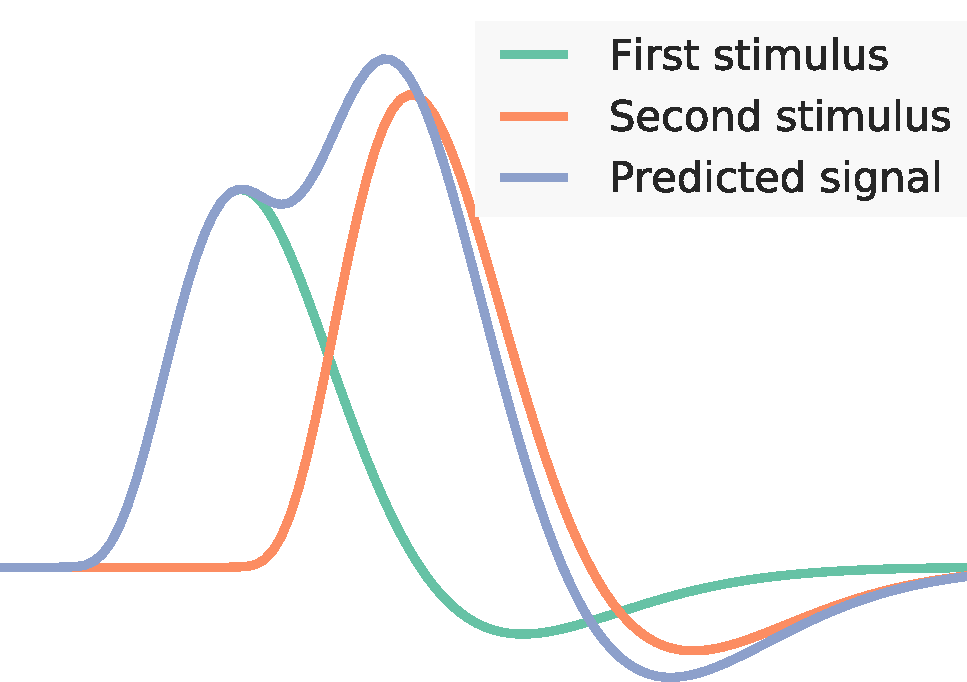
\includegraphics[width=1.\linewidth]{figures/chapter_1/linear_hrf_mini.pdf}
\caption{The general linear model (GLM) predicts that the expected BOLD response to two overlapping stimuli is the sum of the two independent stimuli. In green, the response to the first stimulus that is located at 1 second. In orange, the response to the second stimulus that appears at 6 seconds. In blue, the predicted BOLD response.}\label{fig:1_lti_hrf} 
\end{marginfigure}


% The \emph{Hemodynamic Response Function} (HRF) represents the ideal, noiseless response to an infinitesimally brief stimulus. Different versions of the HRF have been proposed in the literature and in this chapter we examine the characteristic of the HRF used in three different software packages: SPM, AFNI and NiPy.



In order to estimate the activation coefficients, the GLM assumes a \emph{linear time invariant} (LTI) relationship between the BOLD signal and the neural response. This relationship has been reported in a number of studies and can be summarized as $i)$ \emph{Multiplicative scaling}. If a neural response is scaled by a factor of $\alpha$, then the BOLD response is also scaled by a factor of $\alpha$.
\mbox{$ii)$ \emph{Additivity}}. If the response of two separate events is known, the signal for those same events is the sum of the independent signals (Fig.~\ref{fig:1_lti_hrf}).
$iii)$ \emph{Time invariant}. If the stimulus is shifted by $t$ seconds, the BOLD response will also be shifted by this same amount.

The GLM in its classical formulation assumes a known form for the hemodynamic response function (HRF). In Chapter~\ref{chap:hrf_estimation} we will present an extension of the GLM model that estimates jointly the activation coefficients and the hemodynamic response function.


% The General Linear Model (\gls{GLM}) makes use of the knowledge of the hemodynamic response function and linear-time-invariant assumption to model the observed BOLD signal. This model states that the BOLD signal can be expressed in terms of a linear combination of the predicted fMRI responses for different stimuli (also denoted \gls{conditions}) plus a noise term (Fig.~\ref{fig:glm1_abs}). 

% \begin{figure*}[t]
% \center 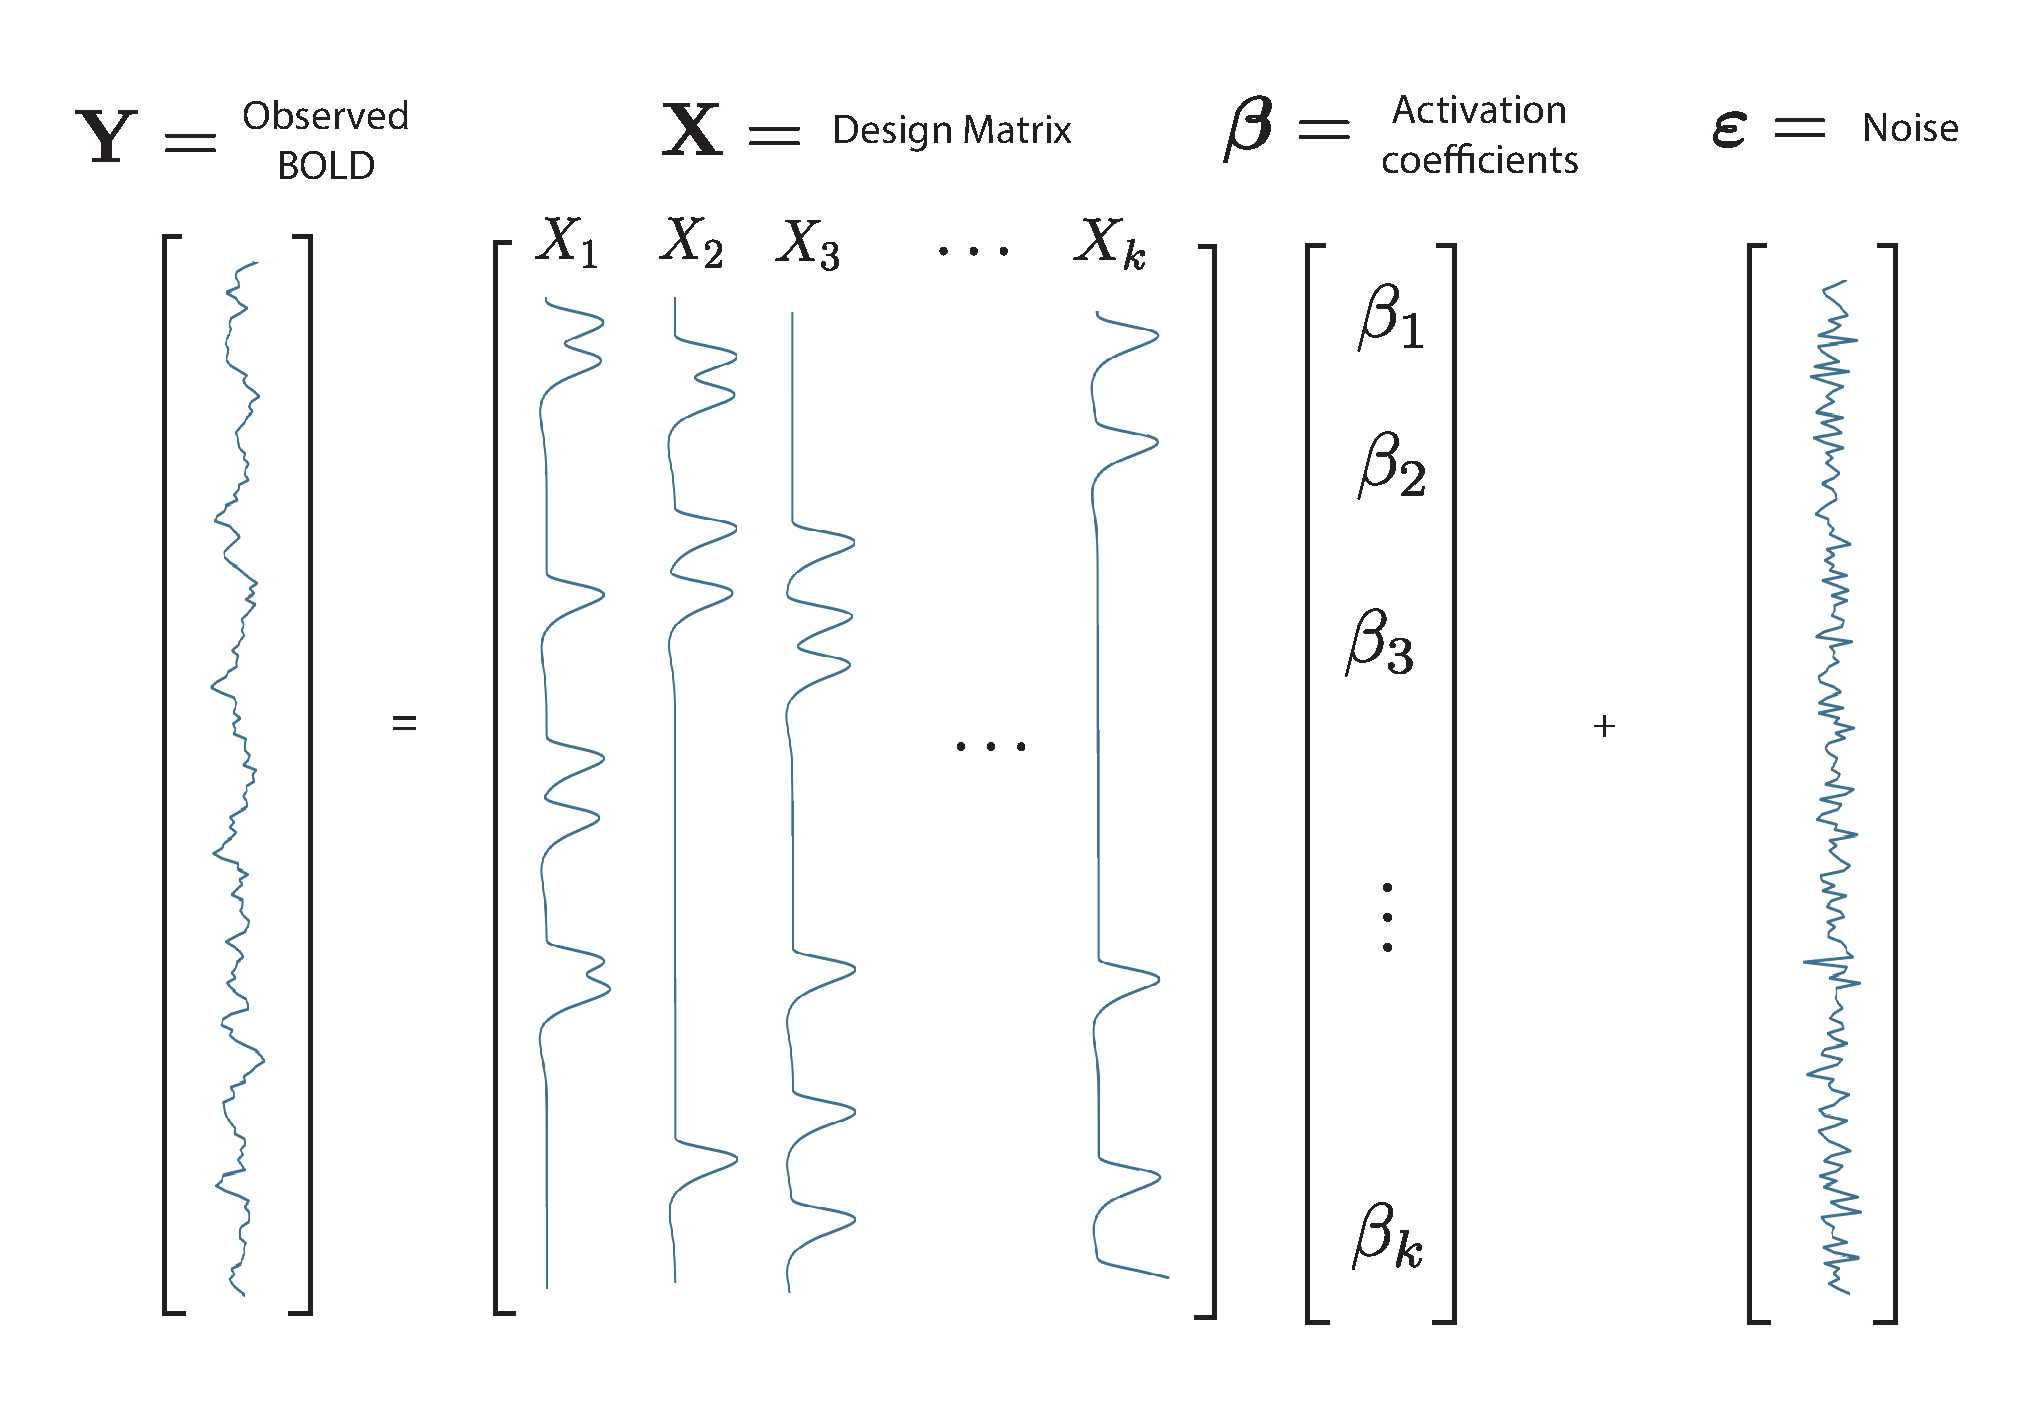
\includegraphics[width=.8\linewidth]{figures/chapter_1/glm_plain.pdf}
% \caption{The GLM expresses the observed BOLD signal as a linear combination of regressors plus an error term. Each regressor of the design matrix is the convolution of a reference HRF and the stimulus function, a function that is 1 when the stimulus is present and zero otherwise. Each element of the (unknown) activation coefficeints represent the relative amplitude of a given condition.}\label{fig:glm1_abs}
% \end{figure*}




\section*{Chapter 3 - Statistical Inference in fMRI}

In this chapter we present the statistical methods that will be used for drawing conclusions from fMRI experiments in further chapters. The chapter is divided into two sections. The first section summarizes the basics of statistical hypothesis testing while the second section describes the basics of supervised machine learning.


Statistical tests can be broadly divided into \emph{parametric} and \emph{nonparametric} tests. Parametric test assume a known probability distribution under the null hypothesis for the distribution parameter that is under consideration. Nonparametric tests do not assume a known form of this probability distribution although they might require some regularity conditions on the distribution such as symmetry. In this chapter  we  describe two parametric statistical tests: the $t$-test and the $F$-test. We will also present a nonparametric test: the Wilcoxon signed-rank test. These tests will be used at different parts of the manuscript. The $t$ and $F$-test will be used to perform voxel-wise inference in section~\ref{subsec:spms} and the Wilcoxon test will be used to compare the performance of different supervised learning models in Chapter~\ref{chap:hrf_estimation}, \ref{chap:decoding_ordinal} and \ref{chap:consistency}.



\begin{marginfigure}
\center 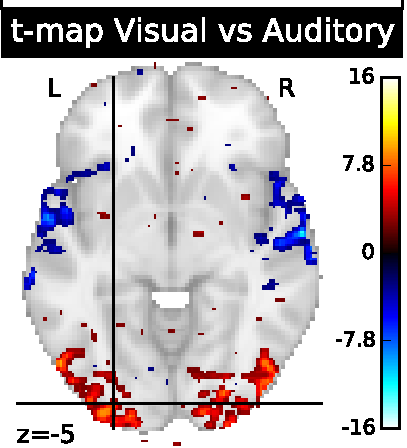
\includegraphics[width=0.8\linewidth]{chapter_2/spm_visual_auditory_mini.pdf}
\caption{Statistical Parametric Maps (SPMs) are images with values that are, under the null hypothesis, distributed according to a known probability density function. In the figure, a $t$-map (i.e. the values are distributed according to a Student $t$ distribution) for a contrast of a Visual vs an Auditory task. Thresholded at $p$-value $< 10 ^ {-3}$. It can be seen how the voxels that exhibit a higher significance of this contrast belong to visual areas (red) and auditory areas (blue)}\label{fig:abs_spm}
\end{marginfigure}

A notable application of parametric statistical tests to fMRI is the creation of Statistical Parametric Maps (SPMs) (Fig.~\ref{fig:abs_spm}). These are images with values that are, under the null hypothesis, distributed according to a known probability density function, usually Student $t$ or the $F$ distribution. To create such maps, one proceeds by performing a parametric test at each voxel. The resulting statistics are assembled into an image - the SPM. 



In the second part of this chapter we introduce different supervised learning models that will be used in subsequent chapters. We will consider models that can be estimated as the solution to a minimization problem of the form
$$
\argmin_{f \in \mathcal{F}} {\mathcal{R}}_n^{\psi}(f) + \lambda \Omega(f) \quad,
$$
where $\mathcal{R}_n^{\psi}(f)$ is a data-fitting term that minimizes a surrogate of the loss function term and $\Omega(f)$ is a regularization term that biases the estimated model towards a set of desired solutions. This way, the model is a trade-off between a data fidelity term and a regularization term. 

We describe different surrogate loss functions and penalties that have found applications in the context of fMRI analysis. The surrogate loss functions that we describe here are Support Vector Machines, Logistic Regression, Support Vector Regression and Least Squares. The penalties that we consider here are squared $\ell_2$, $\ell_1$, elastic-net ($\ell_2^2 + \ell_1$) and total-variation (TV).



Finally, we present two applications of supervised learning to reveal cognitive mechanisms in fMRI studies. The first application is commonly known as \emph{decoding} or \emph{mind reading} and consist in predicting the cognitive state of a subject from the activation coefficients. The neuroscientific questions that decoding is able to address are commonly shaped within the statistical hypothesis testing framework. The inference that we want to establish is whether the classifier trained on data from a given brain area of one subject is accurate enough to claim that the area encodes some information about the stimuli. In this setting, the null hypothesis is that a given brain area does not contain stimuli-related information. The ability of the classifier to correctly predict some information about the stimuli is considered a positive evidence in support of the alternate hypothesis of presence of stimuli-related information within the brain activity. As an application of decoding, we present the dataset~\citep{Borghesani2014}, in which we used decoding techniques to establish in which regions of the brain it is possible to decode different aspects of words representing real-world objects.


A different application is known as \emph{encoding}. Here, the activation coefficients are predicted from some information about the stimuli. The success of an encoding model depends in great measure on our ability to construct an appropriate representation of the stimuli, a transformation that is often nonlinear. For example, \citet{naselaris2009bayesian} constructed two different models for each voxel: a model based on phase-invariant Gabor wavelets, and a semantic model that was based on a scene category label for each natural scene. The authors showed that the Gabor wavelet model provided good predictions of activity in early visual areas, while the semantic model predicted activity at higher stages of visual processing. 


Encoding and decoding can be seen as complementary operations: while encoding uses stimuli to predict activity,  decoding uses activity to predict information about the stimuli. Furthermore, encoding offers the advantage over decoding models that they can naturally cope with unseen stimuli. For example, \citep{Kay2008} used an encoding model to identify natural images that the subject had not seen before. In this case, the predicted activation coefficients were used to select the image that matched most closely the measured activation coefficients.



\begin{fullwidth}
\section*{Chapter~\ref{chap:hrf_estimation} - Data-driven HRF estimation for encoding and decoding models}
\end{fullwidth}


% In this chapter we describe a novel method for the simultaneous estimation of HRF and activation coefficients based on low-rank modeling, forcing the estimated HRF to be equal across events or experimental conditions,
%  yet permitting it to differ across voxels. Estimation of this model leads to
% an optimization problem that we propose to solve with using a
% \mbox{quasi-Newton} method, exploiting fast gradient computations. 
% We compare 10 different HRF modeling methods in terms of encoding and decoding
% score on two different datasets. These results show that the \mbox{R1-GLM} model
% outperforms competing methods in both encoding and decoding
% settings, positioning it as an attractive method both from the points of view
% of accuracy and computational efficiency.


As pointed in Chapter~\ref{chap:intro_fmri}, prior to its use statistical inference procedures, the fMRI data usually goes through \emph{feature extraction} process that converts the BOLD time course into time-independent \gls{activation coefficient}. This is commonly achieved using a model known as Linear General Model (GLM). While
this approach has been successfully used in a wide range of studies, it does
suffer from limitations. For instance, the GLM commonly
relies on a \mbox{data-independent} \emph{reference} form of the hemodynamic response function
(HRF) to estimate the activation coefficient (also known as \emph{canonical} or \emph{reference} HRF). However it is
known that the shape of this response function
can vary substantially across subjects, age and brain regions. This suggests that an adaptive modeling of this
 response function can improve the accuracy of subsequent analysis.



% At a given voxel, it is expected that for similar stimuli the estimated HRF are also 
% similar. Hence, a natural idea is to promote a common HRF
% across the various stimuli (given that they are sufficiently similar), which should result in more robust estimates.
In this work we propose a model in which a common HRF is shared
across the different stimuli that we denote \emph{Rank-1 GLM} (R1-GLM). The novelty of our method stems from the observation that the formulation of the GLM  with a
common HRF across conditions translates to a rank constraint on the vector of estimates. 
This assumption amounts to enforcing the vector of
estimates to be of the form $\bfbeta_{\B{B}} = [\mathbf{h} {\beta}_1, \mathbf{h} \beta_2, \cdots, \mathbf{h}
\beta_k]$ for some HRF $\mathbf{h} \in \RR^d$ and a vector of coefficients $\bfbeta \in \RR^k$. More compactly, this can be written as $\bfbeta_{\B{B}} = \vecop(\B{h}
\bfbeta^T)$. This can be
seen as a constraint on the vector of coefficients to be the vectorization of a rank-one
matrix, hence the name {\it Rank-1 GLM (R1-GLM)}.

In this model, the coefficients have no longer a closed form expression,
but can be estimated by minimizing the following loss function. Given $\B{X}_{\B{B}}$ and $\B{y}$ as before, $\B{Z} \in \RR^{n \times q}$ a matrix of nuisance parameters such as drift regressors, the optimization problem reads:
%
\begin{eqnarray}\label{eq:abs_r1}
\begin{aligned}
\hat{\B{h}}, ~\hat{\bfbeta},~ \hat{\bfomega} ~=~& \argmin_{\B{h}, \bfbeta, {\bfomega}} ~ \frac{1}{2}\|\mathbf{y} - \mathbf{X}_{\B{B}} \vecop(\B{h} \bfbeta^T) - \B{Z} {\bfomega}\| ^2\\
&\text{subject to } \|\B{B} \B{h}\|_{\infty} = 1 \text{ and } \langle \B{B} \B{h}, \B{h}_{\text{ref}}\rangle > 0 \enspace ,
\end{aligned}
\end{eqnarray}

\begin{figure}[t] \centering
\includegraphics[width=.9\linewidth]{chapter_3/scores_recovery_1.pdf}
\includegraphics[width=.9\linewidth]{chapter_3/scores_recovery_2.pdf}
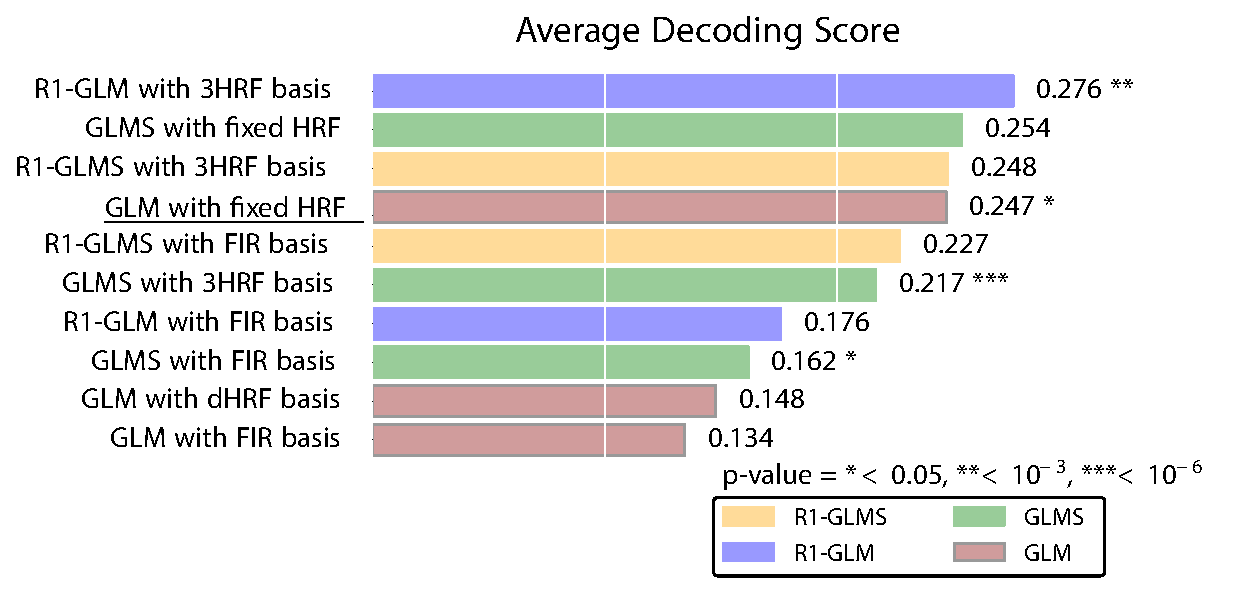
\includegraphics[width=\linewidth]{chapter_3/scores_decoding_smaller.pdf}
\caption{\label{fig:abs_identification_scores} Image identification score (higher is better) on two different subjects from the first dataset and average decoding score on the second dataset. In the first dataset the metric counts the number of correctly identified images over the total number of images (chance level is 1/120 $\approx 0.008$). This metric is less sensitive to the shape of the HRF than the voxel-wise encoding score. The benefits range from 0.9\% points to 8.2\% points across R1-constrained methods and subjects. The highest score is achieved by a R1-GLM method with a FIR basis set for subject 1 and by a R1-GLMS with FIR basis for subject 2.

The metric in the second dataset (decoding task) is Kendall tau. Methods that perform constrained HRF estimation significantly outperform 
methods that use a fixed (reference) HRF. In particular,
the best performing method is the R1-GLM with 3HRF basis, followed by the R1-GLMS with 3HRF basis. 
}
\end{figure}

%
The norm constraint is added to avoid the scale ambiguity between $\B{h}$ and $\bfbeta$
and the sign is chosen so that the estimated HRF correlates
positively with a given reference HRF $\B{h}_{\text{ref}}$.
This ensures the identifiability of the parameters. The optimization problem (Eq.~\eqref{eq:abs_r1}) 
is {\it smooth} and is convex with respect to $\B{h}$, $\bfbeta$ and $\bfomega$,
 however it is not {\it jointly convex} in variables $\B{h}$, $\bfbeta$ and $\bfomega$.



We compare different methods for the joint estimation of HRF and activation coefficients in terms of their score for an encoding and an encoding task. The
methods we considered are standard GLM (denoted \gls{GLM}), a variant of the GLM that improves estimation in highly correlated settings known as GLM with separate designs (GLMS), Rank-1 GLM (R1-GLM) and Rank-1 GLM with separate designs
(R1-GLMS). For all these models we consider different basis sets for
estimating the HRF: a set of three elements formed by the reference HRF and
its time and dispersion derivative, a FIR basis set (of size 20 in the
first dataset and of size 10 in the second dataset) formed by the canonical vectors
and the single basis set formed by the reference HRF (denoted ``fixed HRF''), which
in this case is the HRF used by the SPM 8 software.

We consider two different datasets. The first dataset is presented in~\citep{Kay2008} where it is investigated using an encoding paradigm. The second dataset has been presented in~\citep{Jimura_Poldrack_2011} and is naturally investigated using a decoding paradigm. The scores obtained in both datasets can be seen in Figure~\ref{fig:abs_identification_scores}. In both cases, the proposed method (R1-GLM or its variant R1-GLMS) achieve the highest scores. The results presented in this chapter have been published in~\citep{pedregosa:hal-00952554}.





\vspace{10pt}
\section*{Chapter~\ref{chap:decoding_ordinal} - Decoding with Ordinal Labels}

We have presented in Chapter~\ref{chap:stats_fmri} the decoding problem in fMRI. In this setting it is often the case that the target variable consist of discretely ordered values. This occurs for example when target values consists of human generated ratings, such as values on a Likert scale, size of objects (Fig.~\ref{fig:mini_vb}), the symptoms of a physical disease or a rating scale for clinical pain measurement.


\begin{figure}
\includegraphics[width=\linewidth]{chapter_4/experiment.png}
\caption{In \citep{Borghesani2014}, the authors investigated the possibility to predict different aspects of the words subjects were reading while undergoing an fMRI acquisition. One of the problems we investigated is to predict the size of the objects that the words refer to. In this case, the different stimuli are ordered according to their relative size, i.e. hammer is smaller than cow which is smaller than a whale, etc. In this case, the target variable is of \emph{ordinal nature}. }\label{fig:mini_vb}
\end{figure}


In this chapter we propose the usage of two loss functions to assess the performance of a decoding model when the target consist of discretely ordered values: the absolute error and pairwise disagreement. These two loss functions emphasize different aspects of the problem: while the absolute error gives a measure of the distance between the predicted label and the true label, the pairwise disagreement gives a measure of correct ordering of the predicted labels. These loss functions lead to two different supervised learning problems. The problem in which we seek to predict a label as close as possible to the correct label is known as \emph{ordinal regression} while the problem of predicting ordering as close as possible to the true ordering of a sequence of labels is traditionally known as \emph{ranking}.  

The first models specifically tailored for the problem of ordinal regression date back to the proportional odds and proportional hazards models of~\citep{McCullagh1980}. We present three different surrogate loss functions of the absolute error: least absolute error, ordinal logistic regression and cost-sensitive multiclass classification.


Ranking models were introduced chronologically later than ordinal regression but its popularity has grown in recent years thanks to its applicability to information retrieval (and search engines in particular)~\citep{liu2009learning}. To the best of my knowledge, the first attempt to minimize a convex surrogate of the pairwise disagreement appears is due to~\citet{Herbrich2000}. We consider a model that minimizes a surrogate of the pairwise disagreement: the RankLogistic model. This model can be viewed as a modification of the popular RankSVM model~\citep{Herbrich2000,Joachims2002}.

The choice of either metric (absolute error or pairwise disagreement) will depend on the problem at hand. For example, in clinical applications it is often desirable to predict a label as close as possible to the true label, in which case the absolute error is the appropriate metric. If however, the purpose of the decoding study is to perform a statistical hypothesis test to claim that the area encodes some information about the stimuli, then the pairwise disagreement can be an appropriate measure~\citep{pedregosa2012learning, Borghesani2014, bekhti:hal-01032909}.




% We examine the generalization performance of the presented models on both synthetic data and three fMRI decoding problems from two datasets. We conclude that the best performing models is the last absolute error and ordinal logistic when considering the absolute error as metric and the RankLogistic model when considering the pairwise disagreement as metric. 


\begin{figure*}[t]
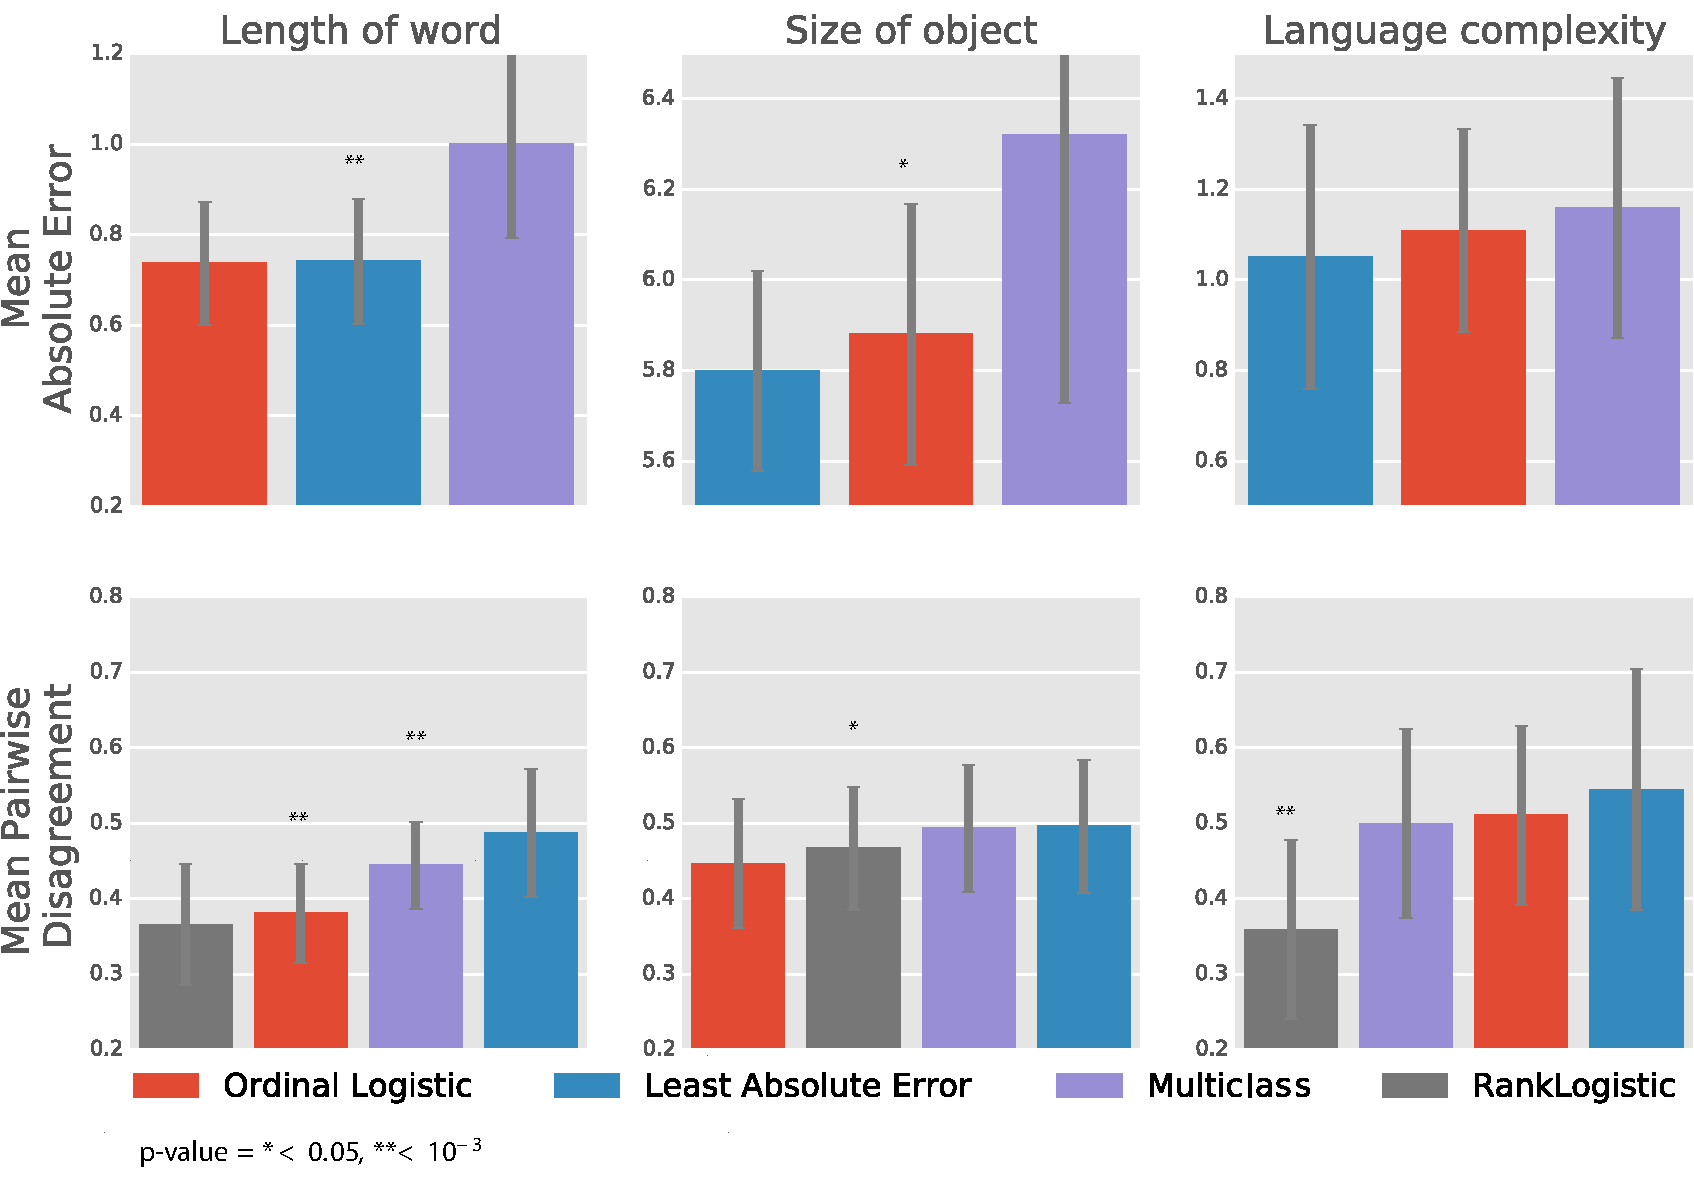
\includegraphics[width=\linewidth]{chapter_4/scores_ordinal.pdf}
\caption[-4cm]{Generalization errors (lower is better) for three fMRI decoding problems. Two different metrics are used corresponding to the rows in the figure: mean absolute error and mean pairwise disagreement. The $*$ symbol represents the $p$-value associated with a Wilcoxon signed-rank test. This test is used to determine whether a given method outperforms significantly the next best-performing method.}\label{fig:abs_scores_ordinal}
\end{figure*}

We examine their generalization error on both synthetic and two real world fMRI datasets and identify the best methods for each evaluation metric (Fig.~\ref{fig:abs_scores_ordinal}). Our results show that when considering the absolute error as evaluation metric, the least absolute error and the logistic ordinal model are the best performing methods. On the other hand, when considering the mean pairwise disagreement the RankLogistic was the best performing method. For neuroimaging studies, this contribution outlines what in our opinion are the best models to choose when faced with a decoding problem in which the target variables are naturally ordered.




\section*{Chapter~\ref{chap:consistency} - Fisher Consistency of Ordinal Regression \mbox{Methods}}


Ordinal regression is the supervised learning problem of learning a rule to predict labels from an ordinal scale. Some ordinal regression models have been  used in Chapter~\ref{chap:decoding_ordinal} to model the decoding problem when the target variable consist of ordered values.

Motivated by its applicability to decoding studies we turn to study some theoretical properties of these methods. The aim is that a theoretical approach can provide a better understanding the methods at hand. For example, \citet{Keerthi2003} proposed two different models for the task of ordinal regression: SVOR with explicit constraints and SVOR with implicit constraints. In that work, the second approach obtained better generalization error in terms of the absolute error loss function. Similar results were obtained by~\citet{lin2006large} replacing the hinge loss by an exponential loss. Yet again, \citet{Rennie} arrived to similar conclusions considering the logistic loss instead. Given these results, it seems natural to ask: is this coincidence or are there theoretical reasons for  this behavior? We will use the result of this chapter to provide an affirmative answer to this last question.
% By the end of the chapter we will be able to affirmatively answer this question.

Many of the ordinal regression models that have been proposed in the literature can be viewed as methods that minimize a convex surrogate of the zero-one, absolute (as outlined in Chapter~\ref{chap:decoding_ordinal}), or squared errors. In this chapter we investigate some theoretical properties of ordinal regression methods. The property that we will investigate is known as \emph{Fisher consistency} and relates the minimization of a given loss to the minimization of its surrogate. 

We consider a rich family of loss functions for ordinal regression. We follow~\citep{Li2007} and determine as admissible loss functions of ordinal regression those that verify the V-shape property, a condition that includes to the best of my knowledge all popular loss functions that have been used in the context of ordinal regression: absolute error, squared error and 0-1 loss. 

In order to introduce the notion of consistency we must fix some notation. In the supervised learning setting, we are given a set of $n$ observations $\{(X_1,
Y_1), \ldots, (X_n, Y_n) \}$ drawn i.i.d.~from $X\times Y$ and a \emph{loss
function} $\ell: \mathcal{Y} \times \mathcal{Y} \rightarrow [0, \infty)$. The goal is to learn from the training examples a measurable mapping called a~\emph{classifier} $h: \XX \rightarrow \mathcal{Y}$ so that the \emph{risk} given below is as small as possible:
\begin{equation}
\label{eq:abs_l_risk}
\mathcal{R}_{\ell}(h) = \EE_{X \times Y}(\ell(Y, h(X)))\quad.
\end{equation}


Attempting to directly minimize the risk is not feasible in practice. First, the probability distribution $P$ is unknown and the risk must be minimized approximately based on the observations. Second, due to the non-convexity and discontinuity of $\ell$, the risk is difficult to optimize and can lead to an NP-hard problem. It is therefore common to approximate $\ell$ by a function $\psi: \mathcal{Y} \times \RR^d \to \RR$, called a \emph{surrogate loss function}, which has better computational properties. The goal becomes to find the \emph{decision function} $f$ that minimizes instead the $\psi$-risk, defined as
\begin{equation}
\Rpsi(f) = \EE_{X \times Y}(\psi(Y, f(X))) \enspace.
\end{equation}



Fisher consistency is a desirable property for surrogate loss functions. It implies that in the population setting, i.e., if the probability distribution $P$ were available, then optimization of the $\psi$-risk would yield a function (not necessarily unique) with smallest possible risk, known as \emph{Bayes predictor} and denoted by $h^*$. This implies that within the population setting, the minimization of the $\psi$-risk and the minimization of the risk both yield solutions with same risk. 
% In other words, consistency implies that the minimization of the $\psi$-risk, which is usually a convex optimization problem and hence easier to solve converges to a solution with minimal $\ell$-risk.

\begin{marginfigure}
\center\textbf{\color{msblue} 0-1 Error}
\includegraphics[width=1.1\linewidth]{chapter_5/probas_or_01.pdf}
\vspace{-30pt}\center\textbf{\color{msblue} Absolute Error}
\includegraphics[width=1.1\linewidth]{chapter_5/probas_or.pdf}
\vspace{-30pt}\center\textbf{\color{msblue} Squared Error}
\includegraphics[width=1.1\linewidth]{chapter_5/probas_or2.pdf}
\caption{
	Bayes predictor can be visualized on the probability simplex. Bayes predictor is a function of the conditional probability $\eta_i(x) = P(y\!=i|X\!=\!x)$. The vector $(\eta_1, \ldots, \eta_k)$ belongs to the probability simplex of $R^n$, which is contained within an hyperplane of dimension $k-1$. In the figure, probability simplex in $\RR^3$ is colored according to the output of Bayes predictor.
}\label{fig:bayes_predictor}
\end{marginfigure}



In this chapter we provide a theoretical analysis of the Fisher consistency properties of a rich family of ordinal regression surrogate loss functions, including proportional odds and support vector ordinal regression. The loss functions that we considered can be divided into three categories: regression-based, threshold-based and classification-based. 


\paragraph{Regression-based loss function. }The \emph{\mbox{regression-based approach}} treats the labels as real values. It uses a standard regression algorithm to learn a real-valued function, and then predicts by rounding to the closest label. In this setting we will examine consistency of two different surrogate loss functions, the absolute error (that we will denote $\psi_{\mathcal{A}}$) and the squared error (denoted $\psi_{\mathcal{S}}$), which are convex surrogates of $\ell_{\mathcal{A}}$ and $\ell_{\mathcal{S}}$, respectively. Given $\alpha \in \RR$, $y \in [k]$, these are defined as
\begin{equation*}
\psi_{\mathcal{A}}(y, \alpha) = |y - \alpha|, \quad \psi_{\mathcal{S}}(y, \alpha) = (y - \alpha)^2 \quad.
\end{equation*}

We prove that the $\psi_{\mathcal{A}}$ surrogate is consistent with respect to the absolute error and that the $\psi_{\mathcal{S}}$ surrogate is consistent with respect to the squared error. Consistency of $\psi_{\mathcal{A}}$ was already proven by~\citep{Ramaswamy2012} for the case of 3 classes. Here we give an alternate simple proof that extends beyond $k>3$. 

\paragraph{\bf Threshold-based loss function.} While the regression-based loss functions may lead to optimal predictors when no constraint is placed on the regressor function space as we will see, in practice only simple function spaces are explored such as linear or polynomial functions. In these situations, the regression-based approach might lack flexibility. \emph{\mbox{Threshold-based} loss functions} provide greater flexibility by seeking for both a mapping $f: \XX \to \RR$ and a non-decreasing vector $\btheta \in \RR^{k-1}$, often referred to as~\emph{thresholds}, that map the class labels into ordered real values. In this context of we consider two different families of surrogate loss functions: the \emph{cumulative link} surrogates and the \emph{margin-based} surrogates. The first family of surrogate loss function that we will consider is the \emph{cumulative link} surrogates. In such models the posterior probability is modeled as $P(Y \leq i|X\!=\!x) = \sigma(g_i(x))$, where $\sigma$ is an appropriate link function. We will prove consistency for the case where $\sigma$ is the sigmoid function, i.e., $\sigma(t) = 1/(1 + \exp(-t))$. This model is known as the \emph{proportional odds} model or \emph{cumulative logit} model~\citep{McCullagh1980}. For $x \in \XX, y \in [k]$ and $\alpha_i = g_i(x)$, the proportional odds surrogate (denoted $\psi_{\mathcal{C}}$) is defined as
\begin{equation}\label{eq:propodds}
\psi_{\mathcal{C}}(y, \balpha) = 
\begin{cases}
-\log(\sigma(\alpha_1)) &\text{ if } y = 1 \\
-\log(\sigma(\alpha_y) - \sigma(\alpha_{y-1})) &\text{ if } 1 < y < k \\
-\log(1 - \sigma(\alpha_{k-1})) &\text{ if } y = k.
\end{cases}
\end{equation}
The other family of surrogates, the margin-based surrogates (denoted $\psi^{\ell}_{\mathcal{M}}$) depends on a V-shaped loss function $\ell$ and is given by
\begin{gather*}
\label{eq:sum_of_loss}
\psi^{\ell}_{\mathcal{M}}(y, \balpha) =
\sum_{i = 1}^{y-1} \Delta \ell(y, i)\phi(\alpha_i) - \sum_{i=y}^{k-1}\Delta \ell(y, i)\phi(-\alpha_i) \enspace.
\end{gather*}
where $\Delta\ell(y, i)$ is the forward difference with respect to the second parameter, defined as $\Delta\ell(y, i) = \ell(y,i+1) - \ell(y, i)$. This formulation parametrizes several popular approaches to ordinal regression. For example, let $\phi$ be the hinge loss and $\ell$ the zero-one loss, then $\psi^{T}_{\ell}$ coincides with the Support Vector Ordinal Regression (``explicit constraints'' variant) of~\citep{Shashua, Chu2007}. If instead the mean absolute loss is considered, this approach coincides with the ``implicit constraints'' formulation of the same reference. For other values of $\phi$ and $\ell$ this loss includes the approaches proposed in~\citep{Shashua,Keerthi2003,Rennie,lin2006large}.

% Since consistency of the threshold-based approach is only proven subject to certain conditions on the underlying probability distribution $P$, we  investigate which are the conditions that guarantee consistency of these surrogates.

\paragraph{\bf Classification-based loss function} Since we aim at predicting a finite number of labels with a specific loss functions, it is also possible to use generic multiclass formulations such as the one proposed in~\citep{lee2004multicategory} which can take into account generic losses. Given $\phi$ a real-valued function, this formulations considers the following surrogate
\begin{equation} \label{eq:multiclass}
\psi_{\mathcal{L}}^{\ell}(y, \balpha) = \sum_{i=1}^k \ell(y, i) \phi(-\alpha_i)
\end{equation}
for $\balpha \in \RR^k$ such that $\sum_{i=1}^k \alpha_i = 0$. The prediction function in this case is given by ${\rm pred}(\balpha) = \argmax_{i \in [k]} \alpha_i$. Note however that this method requires the estimation of $k-1$ decision functions. For this reason, in practical settings threshold-based are often preferred as these only require the estimation of one decision function and $k-1$ thresholds.Consistency results of this surrogate was proven by~\citet{Zhang}, so we will limit ourselves to compare their results to our findings of consistency for threshold-based surrogates in Section~\ref{subsec:multiclass}.





For all the surrogates considered, we either prove consistency or provide sufficient conditions under which these approaches are consistent. Finally, we illustrate our findings by comparing the performance of two methods on 8 different datasets. Although the conditions for consistency that are required by the underlying probability distribution are not necessarily met, we observed that methods that are consistent w.r.t a given loss often outperform other methods that are not consistent with respect to that loss.




\section*{Chapter \ref{chap:conclusion} - Conclusion and Perspectives}

We summarize the contributions of this thesis and point out possible extensions that can be considered in the future. These are:

\begin{enumerate}
\item For the R1-GLM model introduced in Chapter~\ref{chap:hrf_estimation} we outline a possible direction to improve its computational properties by means of tensor factorizations. 

\item For the R1-GLM we outline an approach to consider a common HRF at the parcel level. This would allow the model to take advantage of the spatially dependent nature of fMRI. 

\item The R1-GLM model, being non-convex, comes with no guarantees of convergence to a global optimum for the algorithms considered. We propose to study conditions under which the model is guaranteed to have a unique global optimum.


\item Some of the results presented in Chapter~\ref{chap:consistency} are valid under restrictive conditions on the probability distribution that generates the data. We propose to extend these results to a more general setting by relaxing some of the conditions imposed to achieve consistency of some models.

\item We report the possibility to apply ordinal regression methods to 0-1 multiclass classification. Although ordinal regression methods have been initially developed for loss functions that minimize a distance between the labels (typically the absolute error loss), our theoretical results show that some popular models are instead consistent with the 0-1 loss. This suggest that these methods might be competitive within a multiclass classification setting. A potential advantage of these methods compared to other multiclass classification methods is the lower amount of parameters to estimate.
\end{enumerate}




% Afin d'estimer les coefficients d'activation, le GLM suppose une relation linéaire invariant de temps (LTI) entre le signal BOLD et la réponse neurale. Cette relation a été rapporté dans un certain nombre d'études et peut être résumée comme i) mise à l'échelle multiplicatif. Si une réponse neurale est réduite par un facteur de α, alors la réponse BOLD est également mis à l'échelle par un facteur de α. ii) d'additivité. Si la réponse à deux événements distincts est connu, le signal de ces événements se ils devaient se produire à proximité dans le temps est la somme des signaux indépendants (Fig. 2.1). iii) Durée invariant. Si le stimulus est décalée de t secondes, la réponse BOLD sera également décalé de ce même montant.
% Le GLM dans sa formulation classique prend une forme connue pour la fonction de réponse hémodynamique (FRH). Dans le chapitre 5, nous allons présenter une extension du modèle GLM qui estime conjointement les coefficients d'activation et la fonction de réponse hémodynamique.



\newpage

\begin{fullwidth}
\bibliographystyle{plainnat}
\bibliography{abstract}
\end{fullwidth}



\chapter{Introduction to Functional MRI}\label{chap:intro_fmri}
\markright{{~{\rm \ref{chap:intro_fmri}}. Introduction to fMRI}\hfill}{}

\label{Chapter_1}



\vspace*{\fill}
\newthought{In this chapter} we introduce functional magnetic resonance imaging (fMRI). We will start by providing some insight into human brain structure and function. Then, we will introduce the principal brain imaging techniques in use nowadays. Different imaging techniques can be used to answer different neuroscientific questions. Functional MRI, due to its good spatial resolution and whole brain coverage is specially well suited to answer questions relating the localization of brain activity for a given task.

Before the data acquired through fMRI can be used in statistical analysis it has to go through a  preprocessing pipeline. In the last part of this chapter we detail the different steps of this pipeline, with special emphasis on the general linear model (GLM), a model that allows to extract time-independent activation coefficients from the fMRI time series in event-related designs.  These activation coefficients will form the basis of statistical studies presented in later chapters. 

% In the last part of the chapter we focus on fMRI and we relate the different steps from the scanner images to the statistical studies of later chapters.

% The objective of cognitive studies relating the brain's structure to its function is the output of time-independent activation maps for a given task. We will present a model, known as general linear model (GLM) .


% {\blue
% fMRI consist of successive  brain scans, given in intervals ranging from 1 to 4 seconds. However,  Because of the inherent delay of oxygen consumption in the brain, construction of these maps is not straightforward in the case of fMRI for fast event-related designs. We will describe a model known as general linear model (GLM) that .
% }

\hspace{20pt}
\minitoc
\vspace*{\fill}

\newpage


\section{General brain structures}\label{Chapter_1_Section_1}



The human brain has a volume of around $1200 \; cm^3$ and an average weight  of 1.5 kg. It is composed of neurons, glia cells and blood vessels. Glia cells are responsible for the structural and metabolic support of neurons. About $86$ billion neurons~\citep{Azevedo2009} process and transmit information through electrical and chemical signals. The information is transmitted along the neuron by \emph{action potentials}
(also called \emph{spikes}), that are short-lasting electrical events in which
the electrical membrane potential of a cell rapidly rises and falls. 

\begin{marginfigure}[-0.5cm]
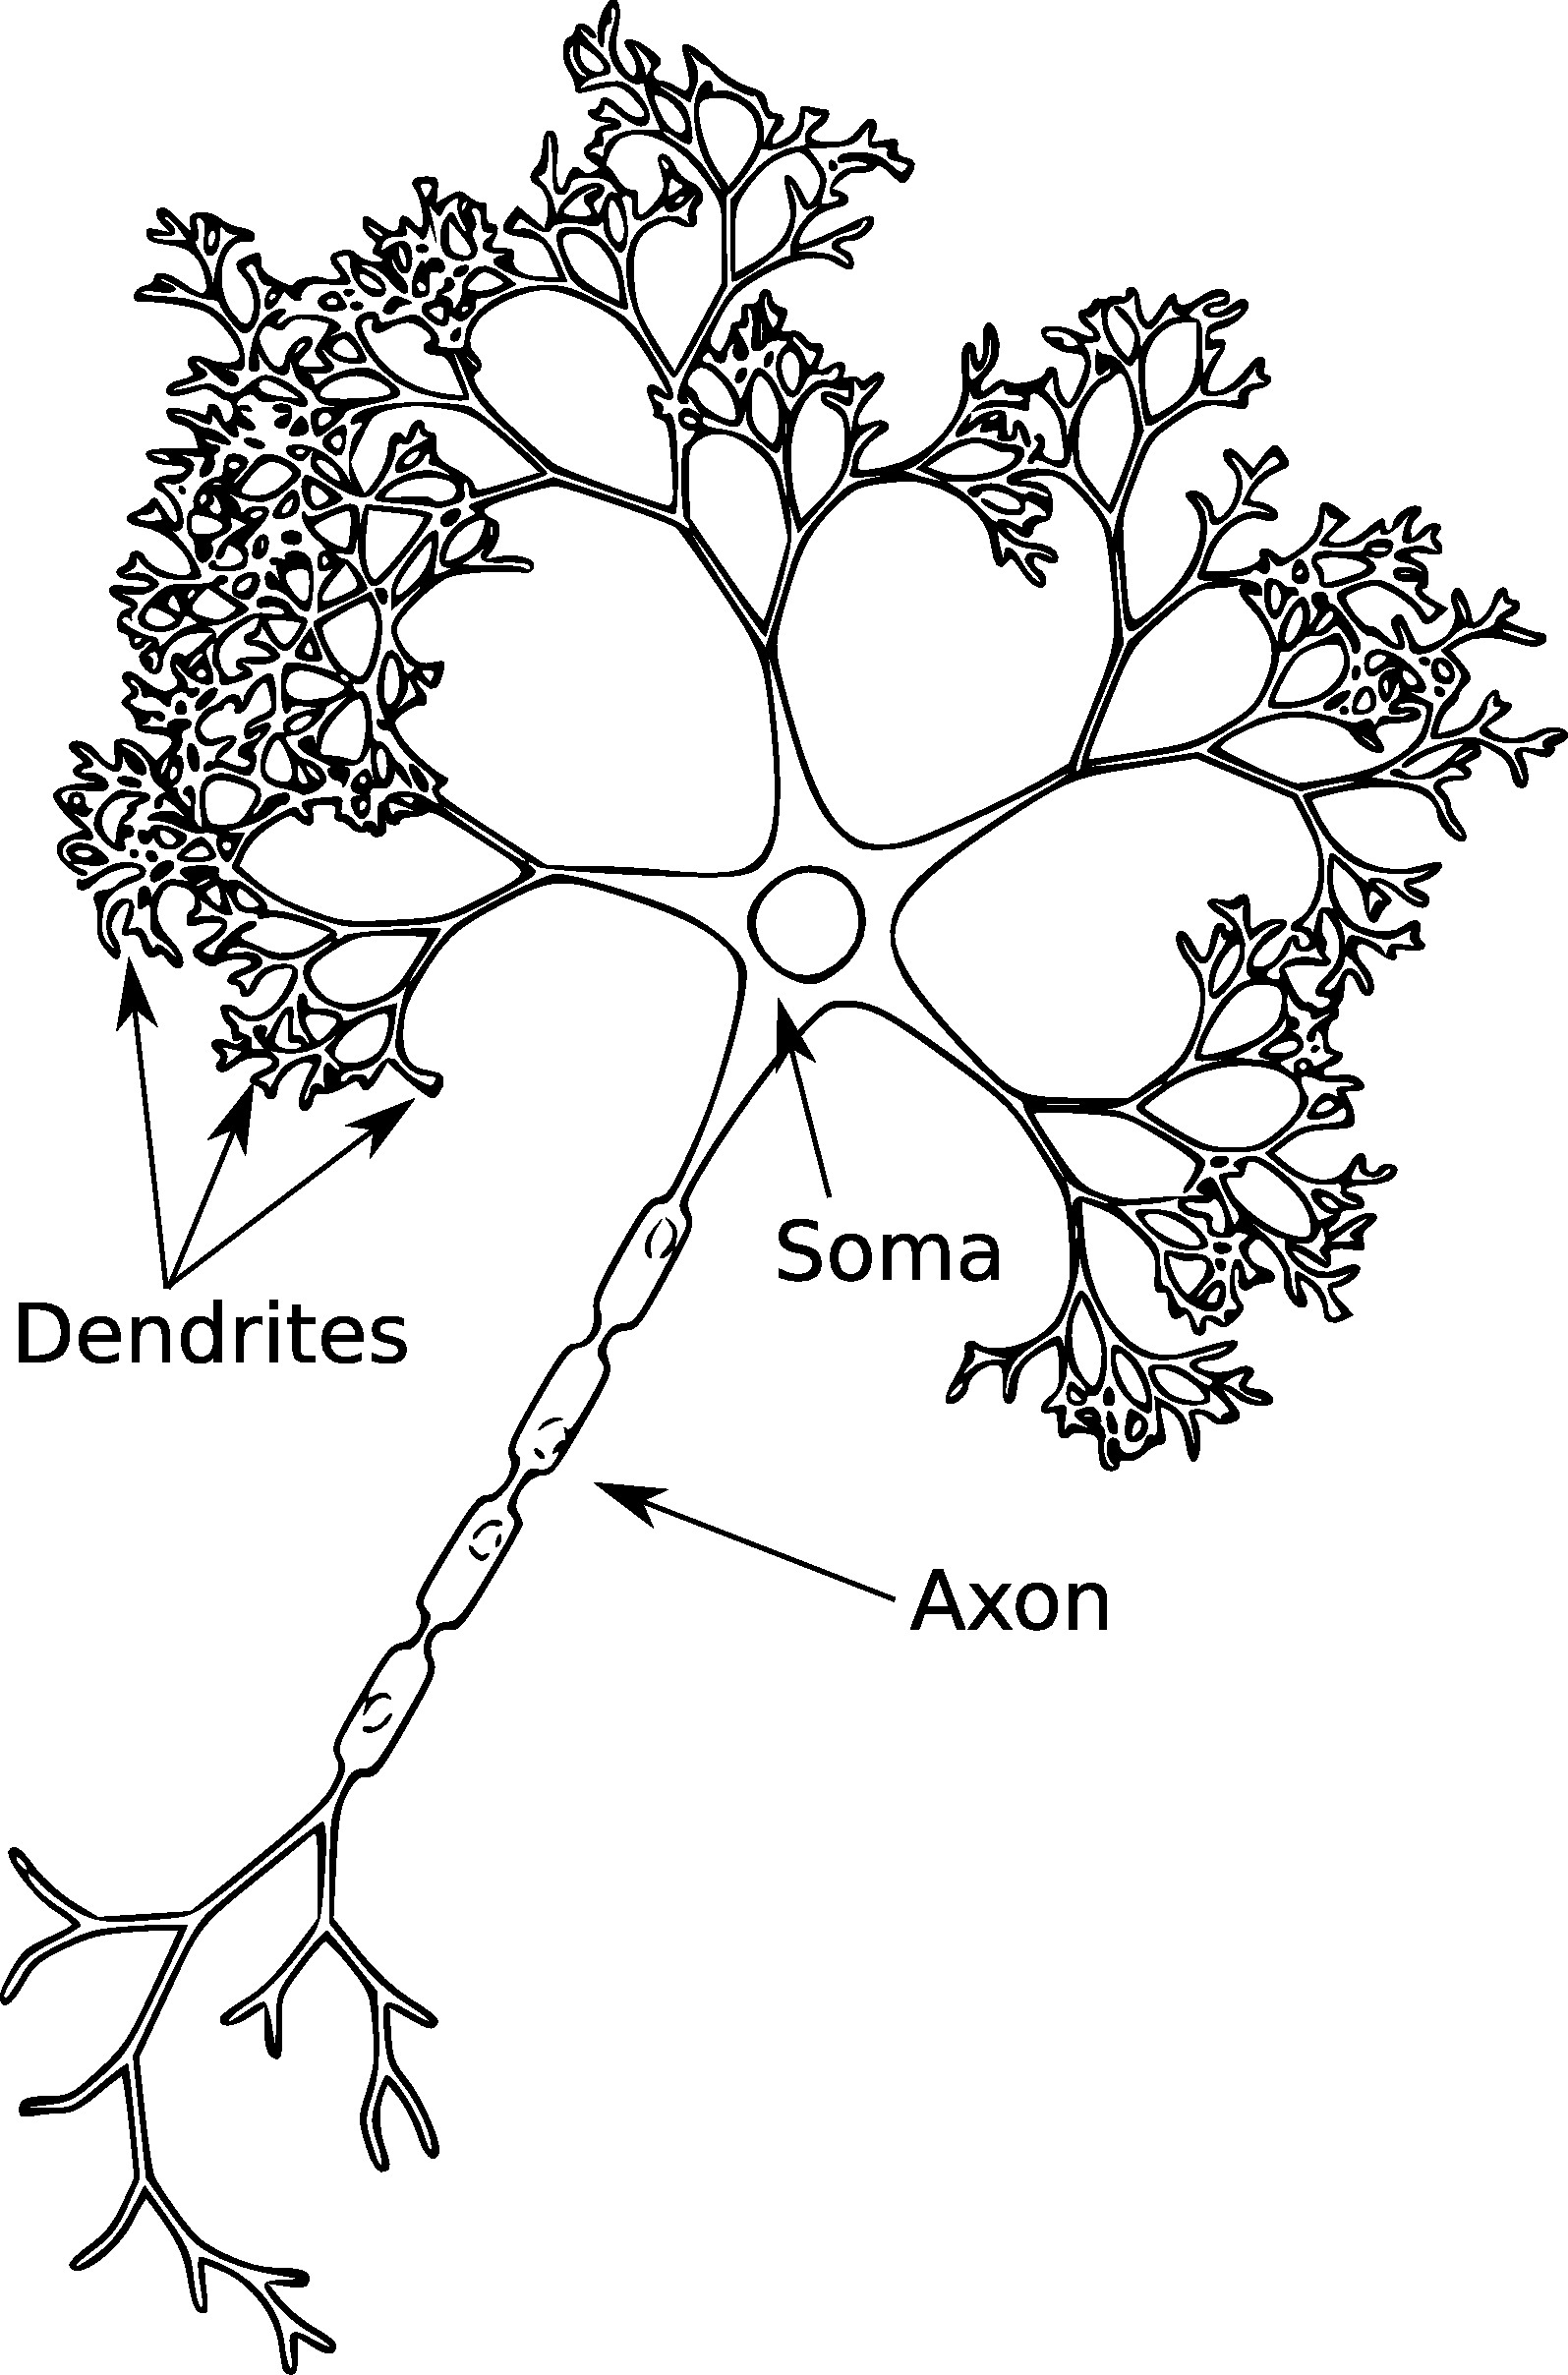
\includegraphics[width=1.0\linewidth]{chapter_1/chapter_1_neuron.pdf}
\vspace{-20pt}\caption{
Schematic view of a neuron, in scale $10^{5}:1$. A neuron has a cell body (\emph{soma}), many regions for receiving information from other neural cells (\emph{dentrites}) and often a nerve fiber called \emph{axon}.
Adapted from http://commons.wikimedia.org/.}\label{fig:chapter_1_neuron}
\end{marginfigure}


A neuron (Fig.~\ref{fig:chapter_1_neuron}) has a cell body (called the \emph{soma}), many regions for
receiving information from other neural cells (called \emph{dendrites}),
and
often an \emph{axon} (\emph{nerve fiber}) for transmitting information to
other
cells. Neurons communicate with one another via chemical synapses, where the axon terminal of one cell impinges upon another neuron's dendrite, soma or, less commonly, axon. Neurons can have over 1000 dentritic branches, making connections with tens of thousands of other cells. Synapses can be excitatory or inhibitory and either increase or decrease activity in the target neuron. Some neurons also communicate via electrical synapses, which are direct, electrically conductive junctions between cells.

\begin{marginfigure}[0.5cm]
\includegraphics[width=1.\linewidth]{chapter_1/Cajal-shadow.jpg}
\vspace{-10pt}\caption{
	Santiago Ramón y Cajal (Navarre, Spain 1852 – Madrid, Spain 1934) is widely regarded as the father of modern neuroscience. Cajal and italian anatomist Camillo Golgi impersonated the dispute between neuron and reticular theory at the turn of the 20th century. They received a joint Nobel Prize in Physiology and Medicine in 1906.
}
\end{marginfigure}



The human brain can be decomposed in two parts: the \emph{white matter}, constituted by the nerve
fibers, and the \emph{gray matter} constituted by the neural cell bodies.
The surface of the human brain is a highly circonvoluted 6-layered structure
called \emph{neocortex} (or more simply \emph{cerebral cortex}). This layer is folded in a way that increases the amount of surface that can fit into the volume available. A cortical fold is called \emph{sulcus}, and the area between two \emph{sulci} is called a \emph{gyrus}.


The human cortex is often divided into four ``lobes'', called the frontal lobe, parietal lobe, temporal lobe and occipital lobe (see Figure~\ref{fig:chapter_1_functions}). The left and right side hemispheres of the cortex are broadly similar in shape, and most cortical areas are replicated on both sides. Some areas, however, show strong lateralization, such as areas that are involved in language, located in the vast majority of subject in the left hemisphere.

% \begin{marginfigure}
% \includegraphics[width=1.\linewidth]{figures/640px-Phrenology-journal.jpg}
% \caption{Front page of the Americal Phrenological Journal, 1848. Although now considered a pseudoscience, phrenological thinking has been influential in 19th-century psychiatry and modern neuroscience}
% \end{marginfigure}

How the different anatomical structures of the brain correspond to the neural substrate of cognitive functions is one of the oldest debates in neuroscience, defining an entire field: cognitive neuroscience. The idea of linking a given cognitive function to a specific brain region can be traced back to the work of nineteen century phrenologists, who based their localizationist attempts on the shape of the skull. In the 20th century, a group of neuropsychologists, in absence of direct means to investigate brain activity, studied patients with cortical damages observing that some focal lesions were associated with relatively global effects on behavior. This lead them to argue against a strictly localizationist view of brain organization. Nowadays it is widely recognized that the activity of specific brain regions underlie many cognitive functions (e.g.vision, in occipital areas). At the same time, the relevance of \emph{brain networks} encompassing different anatomical regions for the multimodal integration of features necessary for higher level cognitive functions (e.g.attention in the fronto-parietal network) ~\citep{gazzaniga2004cognitive} has been acknowledged.


\begin{figure}
\begin{center}
\center 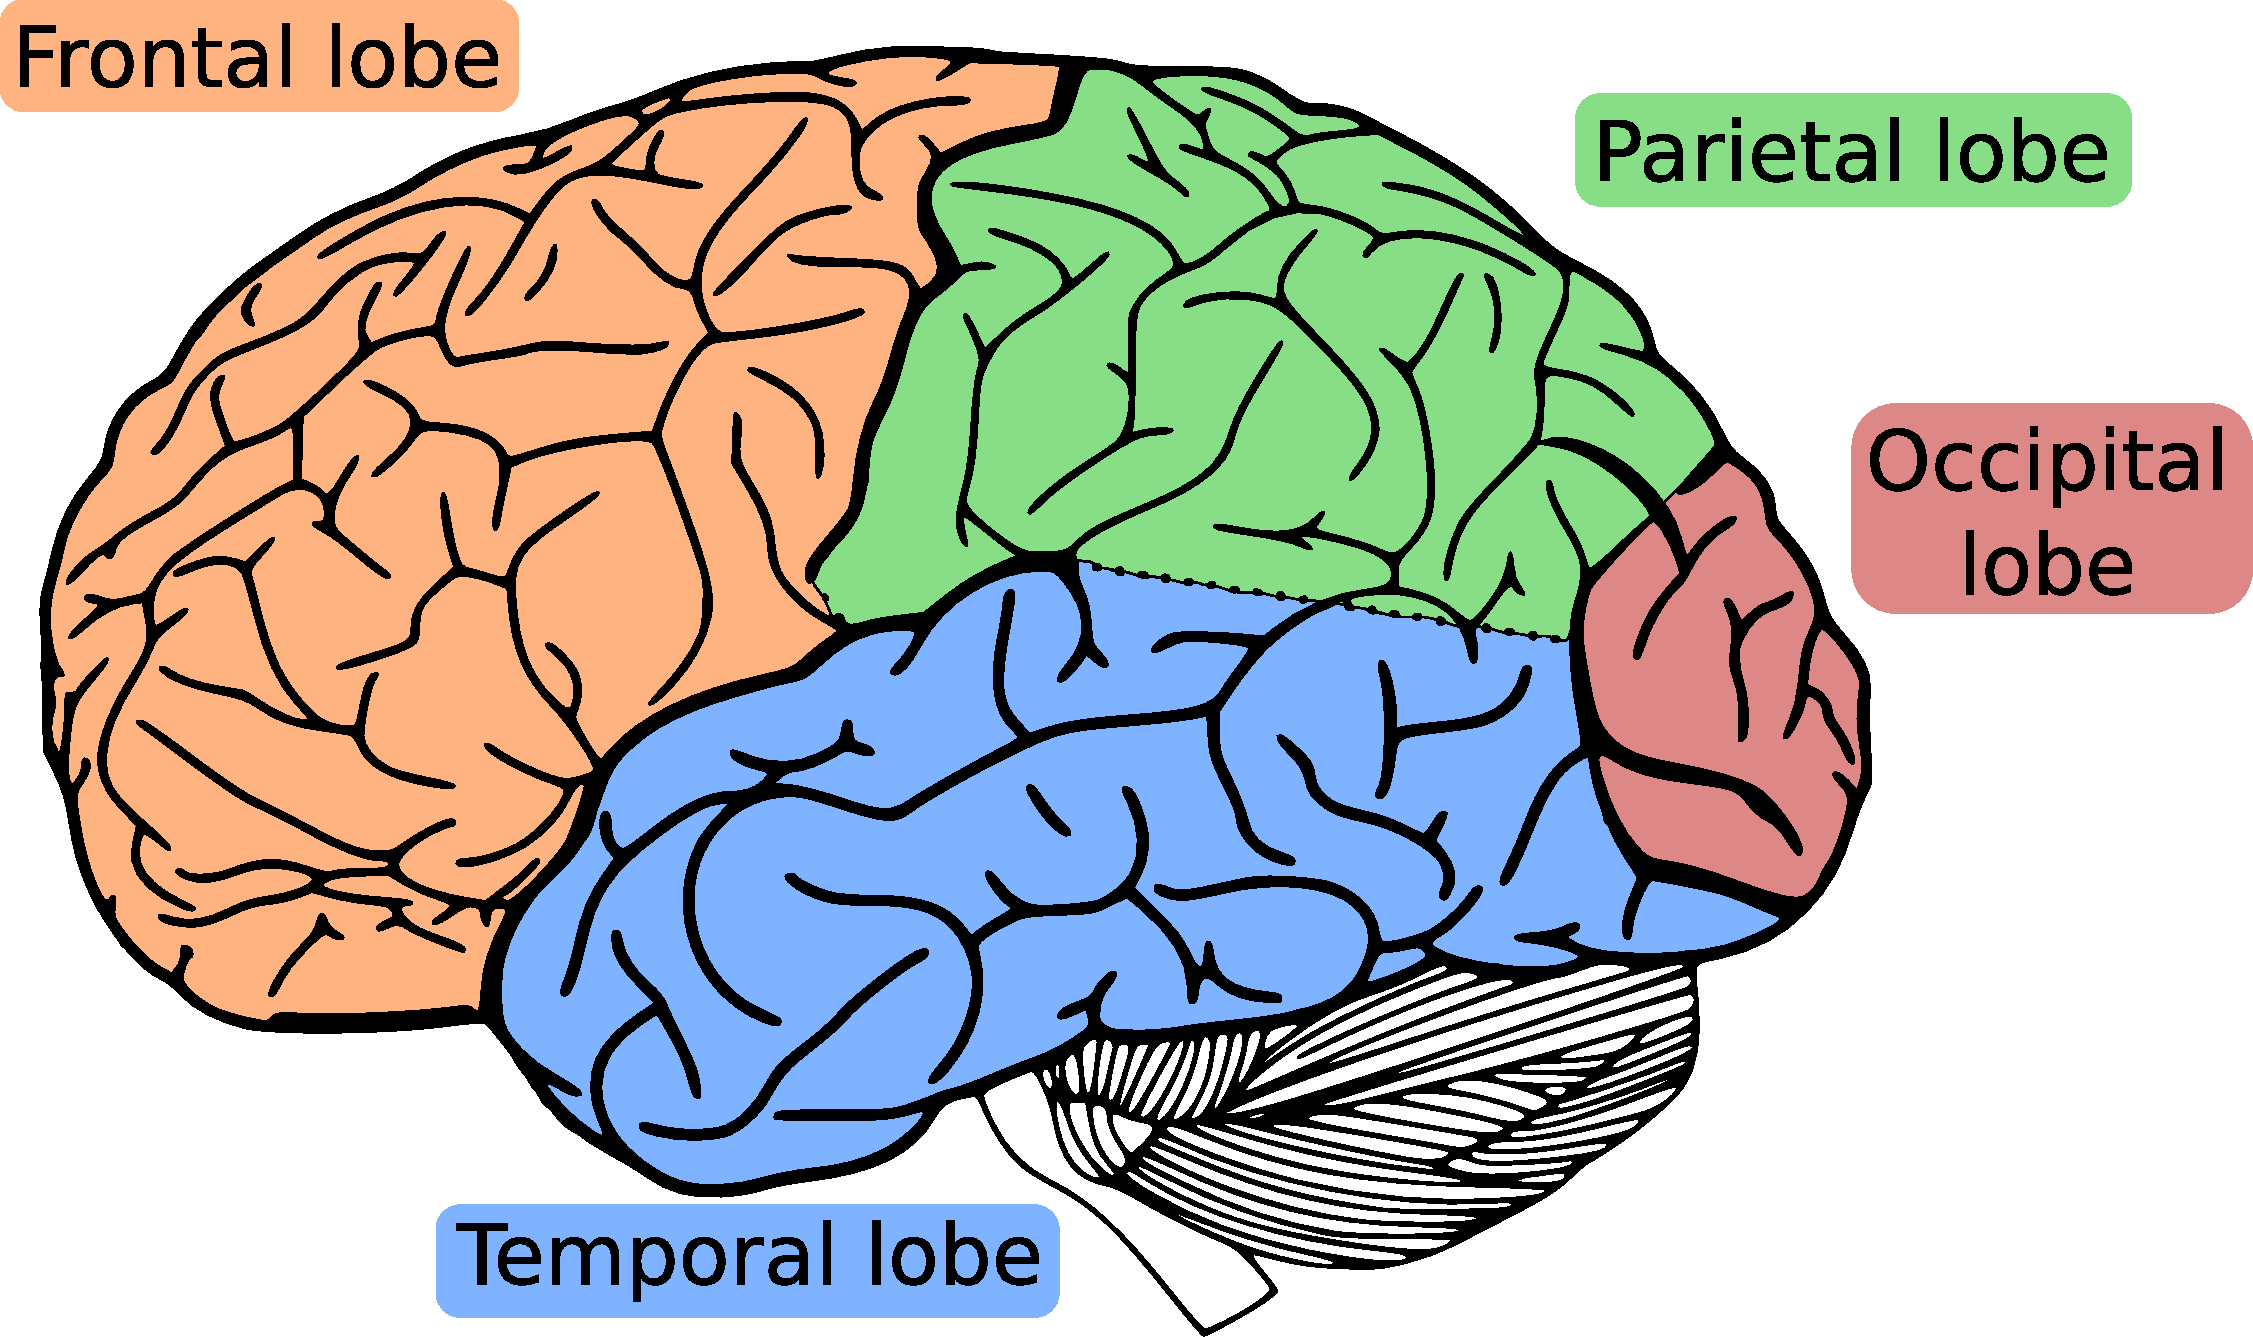
\includegraphics[width=0.6\linewidth]{chapter_1/chapter_1_lobe.pdf}
\center 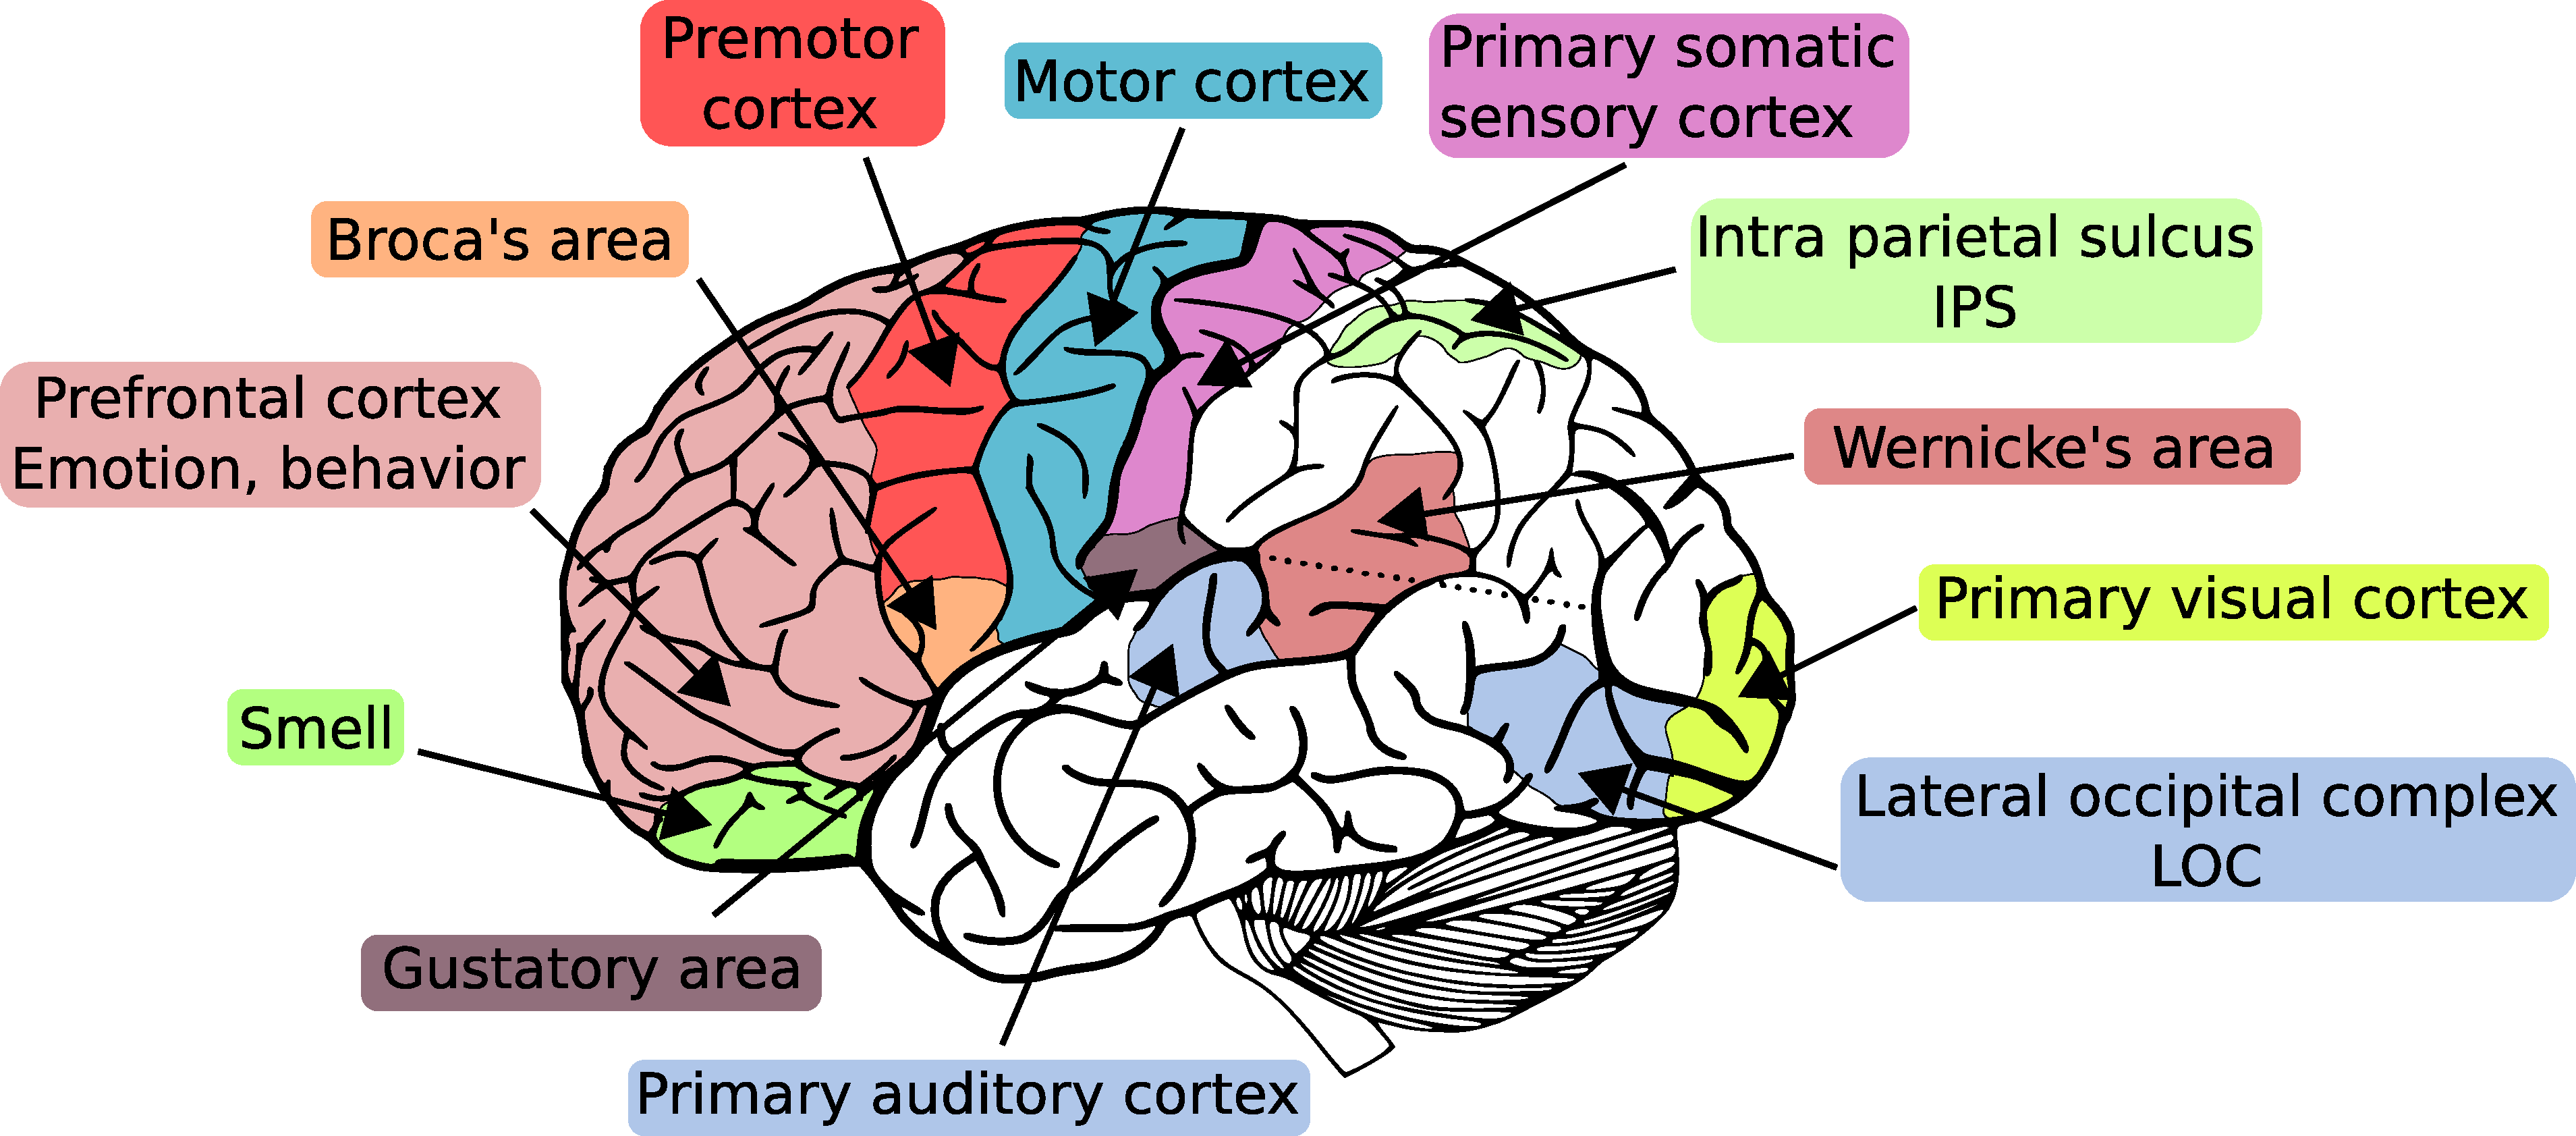
\includegraphics[width=1.\linewidth]{chapter_1/chapter_1_functions.pdf}
\end{center}
\caption{Lobes and some functional regions
of the human brain (left hemisphere).
Within each lobe are numerous cortical areas, each associated with a particular function such as
sensory areas (\emph{e.g. visual cortex, auditory cortex}) that receive and
process information from sensory organs, motors areas (\emph{e.g. primary motor
cortex, premotor cortex}) that control the movements of the subject,
and associative areas (\emph{e.g. Broca's area, Lateral Occipital Complex -- LOC
--
or Intra Parietal Sulcus -- IPS --}) that process the high-level information
related to cognition. The experiments detailed in this thesis are related to
object recognition (\emph{visual cortex} and \emph{LOC}) and number processing
(\emph{parietal cortex} and \emph{IPS}). Source: adapted from \citep{michel2010understanding}.}\label{fig:chapter_1_functions}. 
\end{figure}




\section{Functional neuroimaging modalities}

Until the advent in the 1920s of non-invasive neuroimaging modalities, most of the accumulated knowledge of the brain came from the study of lesions, post-mortem analysis and invasive experimentations. With the advent of modern, non-invasive imaging techniques, several aspects of the human brain are revealed in vivo with high degree of precision.

Several brain imaging techniques are available today. These can be divided into \emph{structural} or \emph{anatomical} and \emph{functional} imaging techniques. While structural imaging provides details on morphology and structure of tissues, functional imaging reveals physiological activities such as changes in metabolism, blood flow, regional chemical composition, and absorption. In this section we will discuss briefly the main functional neuroimaging modalities available today.

\begin{itemize}
\item{\bf {Electroencephalography - EEG}}
% \begin{marginfigure}[3cm]
% \center \includegraphics[width=.8\linewidth]{figures/eeg2.jpg}
% \caption{EEG Cap}
% \end{marginfigure}
is a widely used modality for functional brain
imaging. \emph{EEG} measures electrical activity along the scalp. EEG activity  reflects the synchronous activity of a population of neurons that have similar spatial orientation. If the cells do not have similar spatial orientation, their ions do not line up and thus do not create detectable waves. Pyramidal neurons of the cortex are thought to produce most of the EEG signals because they are well-aligned and fire together. Because voltage fields fall off with the square of distance, activity from deep sources is more difficult to detect than currents near the skull. Due to the ill-posed problem of
volumetric data reconstruction from surface measurements,
\emph{EEG} has a poor spatial resolution compared to other modalities
such as \emph{fMRI}.

\item{\bf {Stereotactic electroencephalography - sEEG}} is an invasive version of
\emph{EEG}, based on intra-cranial recording. It measures the electrical
currents
within some regions of the brain using deeply implanted electrodes, localized
with a stereotactic technique.
This approach has the good temporal resolution of \emph{EEG} and enjoys an
excellent spatial resolution. However, \emph{sEEG}
is very invasive and is only performed for medical purpose (\emph{e.g}
localization of epilepsy foci) and has a limited coverage (only the regions with electrodes).
A close approach is \emph{Electrocorticography -- ECog --} that uses
electrodes placed directly on the exposed surface of the brain. Even in this case its usage is restricted to medical purposes.


\begin{marginfigure}[5cm]
\center \includegraphics[width=1.\linewidth]{chapter_1/meg.pdf}
\caption{Magnetic field measured with MEG on a somato-sensory experiment. It is a 2D topography 20 ms after stimulation. Source: \citep{gramfort:09}}
\end{marginfigure}
\item{\bf{Magnetoencephalography - MEG}}
measures the magnetic field induced by neural electrical activity.
The synchronized currents in neurons create magnetic fields of a
few hundreds of femto Tesla ($fT$) that can be detected using specific devices. 
Although EEG and MEG signals originate from the same neurophysiological processes, there are important differences. Magnetic fields are less distorted than electric fields by the skull and scalp, which results in a better spatial resolution of the MEG. Whereas EEG is sensitive to both tangential and radial components of a current source in a spherical volume conductor, MEG detects only its tangential components. Because of this EEG can detect activity both in the sulci and at the top of the cortical gyri, whereas MEG is most sensitive to activity originating in sulci. EEG is, therefore, sensitive to activity in more brain areas, but activity that is visible in MEG can be localized with more accuracy. Note that EEG and MEG can be measured simultaneously.


\item{\bf{Positron emission tomography - PET}}
 is an imaging modality based on the
detection of a radioactive tracers introduced in the body of the subject. The
tracers (or \emph{radionuclide} decay) emit a positron which can in turn emit,
after recombination with an electron, a pair of photons that are detected
simultaneously. PET therefore provides a quantitative measurement of the physiological activity. It can also be used for functional imaging, by choosing a specific tracer.
In particular, the \emph{fluorodeoxyglucose} (or \emph{FDG}), is used for
imaging the metabolic activity of a tissue. This is based on the assumption that areas of high radioactivity are associated with brain activity.
\emph{PET} has two major limitations: the tracers required for
\emph{PET} are produced by cyclotrons (a type of particle accelerator),
which implies an heavy logistic. Furthermore, the use of radio-tracers is not harmless
for the
health of the subjects so \emph{PET} is now used for medical purpose only.

\begin{marginfigure}[0cm]
\center \includegraphics[width=.8\linewidth]{chapter_1/212px-PET-image.jpg}
\caption{PET scan of a human brain. 
PET measures indirectly the flow of blood to different parts of the brain, which is, in general, believed to be correlated with neural activity.
Souce: wikipedia.org}
\end{marginfigure}


\item{\bf{Single photon emission computed tomography - SPECT}} is an imaging modality based on the detection of a radioactive tracer. SPECT is similar
to \emph{PET} in its use of radioactive tracer material. However, the
measure in \emph{SPECT} is the direct consequence of the tracer (the tracer
emits gamma radiation), where \emph{PET} is based on an indirect consequence of
the tracer (positron then gamma radiation). The spatial resolution is slightly worse
than \emph{PET}.
%
\emph{SPECT} can be used for functional brain imaging, by using a specific
tracer which will be assimilated by the tissue in an amount proportional to
the cerebral blood flow.


\item{\bf{Near-infrared spectroscopy - nIRS}}
 is a recent modality for
medical imaging. \emph{nIRS} is based on the fact that the absorption of the
light in the
near-infrared domain contains information on the blood flow and blood
oxygenation level. It is non-ionizing (harmless), and the instruments are
not too expensive. However, the spectra obtained by \emph{nIRS} can be difficult
to interpret, and this technique, which requires a complex calibration, measures
signals only close to the outer layer of the cortex.

\newglossaryentry{fMRI}{name=fMRI,description=Functional Magnetic Resonance Imaging}

\item{\bf{Functional MRI} -- {\gls{fMRI}}} is
a widely used method for functional brain imaging, because it is
non-invasive, has a good spatial
resolution ($1mm^3$), and provides access,
albeit indirectly, to the neural activity.
Moreover, in standard acquisitions, \emph{fMRI} yields a
full-brain coverage, as it does not
restrict the study to superficial layers or predefined regions of the cortex.

\end{itemize}


Different modalities have different trade offs in terms of spatial and temporal resolution. For example, EEG and MEG enjoy temporal resolutions of the order of few miliseconds and are thus well suited for studies of temporal dynamics of information processing but have limited spatial resolution. On the other hand, fMRI enjoys a better spatial resolution but the temporal resolution is around 1 second. Furthermore, as we will see in the next section, temporal resolution in fMRI is further limited by the slow spread of hemodynamic response, which lasts around 20 seconds after the stimuli presentation.




\begin{figure}[h!tb]
\center \includegraphics[width=0.8\linewidth]{chapter_1/chapter_1_methods.pdf}
\caption[Spatial and temporal resolutions of the different modalities commonly
used for functional imaging]{Spatial and temporal resolutions of different
modalities commonly
used for functional imaging. A typical fMRI acquisition (as of 2014) enjoys spatial resolution of the order of {$1-3mm^3$} and temporal resolution of the order of 1-3 seconds.}\label{fig:chapter1_methods}
\end{figure}

Certain imaging techniques are more adapted than other to answer certain neuroscientific questions. Due to its good spatial resolution and whole brain coverage, fMRI is particularly well adapted to \emph{localize} the effect of a certain experimental condition. This task is not reduced to the construction of brain maps, but also involves the understanding of the underlying brain connectivity~\citep{johansen2005functional,behrens2006consistent} and the effects regions exert on each other in a certain experimental context~\citep{pessiglione2007brain, behrens2007learning}. One of the main hopes in functional imagining is that it might be used as an objective diagnosis tool for several diseases. In particular, the aim is to find some \emph{biomarkers} for psychiatric diseases by comparing different population of patients: this is the case for autism, schizophrenia or Alzheimer's disease. 


\section{Functional MRI and BOLD signal}


\newglossaryentry{MRI}{name=MRI,description={{Magnetic Resonance Imaging}}}



The primary form of fMRI measures the oxygen change in blood flow. This is known as the Blood-oxygen-level dependent (BOLD) contrast. Other increasingly popular functional MRI method is arterial spin labeling (ASL)~\citep{detre1994tissue, alsop1998multisection, williams1992magnetic}, which uses arterial water as tracer to measure cerebral blood flow. Compared to fMRI, ASL has a lower signal to noise ratio~\citep{detre2002technical}. However, ASL provides reliable absolute quantification of cerebral blood flow with higher spatial and temporal resolution than other techniques~\citep{borogovac2012arterial}. This thesis specifically considers BOLD functional MRI and through the manuscript we use the name functional MRI (fMRI) to denote functional MRI based on the BOLD signal.

\newglossaryentry{bold}{name=BOLD,description={{fMRI contrast that measures oxygen change in blood flow}}}

%
The \emph{\gls{bold}} contrast can be explained by considering a protein present in
the blood
cells, called hemoglobin. Hemoglobin can bind with oxygen in order to bring it
into the different cells of the organism, this link being reversible and
unstable. Thus, it can be found in two different forms: \emph{oxyhemoglobin}
($Hb-O_{2}$ - giving a bright red color to the blood), its oxygenated form, and
\emph{deoxyhemoglobin} ($Hb$ - giving a blue-purple color to the blood), its
deoxygenated form.
%
%
%
%
When the \emph{oxyhemoglobin} loses its oxygen atoms and
becomes the \emph{deoxyhemoglobin}, it becomes more affected by an externally applied magnetic field (due to the iron
oxides). The presence of
\emph{deoxyhemoglobin} in the blood modifies the
magnetic resonance signal of the protons of the water molecules surrounding the blood
vessels. 

\begin{figure}
\centering
\includegraphics[width=1.\linewidth]{chapter_1/chapter_1_bold.png}
\caption[][-2.5cm]{
Illustration of the effect of the $CO_2$ on the \emph{BOLD} contrast.
Left - Coronal slice showing the \emph{BOLD} contrast of an anesthetized rat
which has breathed pure $O_2$. Right - Coronal slice of the same rat, showing the \emph{BOLD} contrast after respiration of a mixture of $90\%$ of $O_2$ and $10\%$ of $CO_2$ (this mixture
increases the oxygenation of the venous blood). The arrow shows 
the sagittal sinus, which is one of the major veins of the brain. This picture shows a strong increase of intensity in this vein, that illustrates that the
variation of blood oxygenation is visible in \emph{BOLD} contrast.
Adapted from \citep{ogawa1990b}.}\label{fig:chapter_1_ogawa}
\end{figure}


The difference of magnetic
susceptibility between the
blood vessel and the surrounding tissues creates 
inhomogeneities in the magnetic field \citep{thulborn1982,ogawa1990a} that are quantified by the magnetic resonance scanner. In the seminal paper \citep{ogawa1990b} studied the variations of
\emph{BOLD} contrast in the brain of an anesthetized rat during the inhalation of a gas
 that increases the \emph{cerebral blood flow} (\emph{CBF}), and thus blood
oxygenation (see Figure
\ref{fig:chapter_1_ogawa}).

\newglossaryentry{voxel}{name={voxel},description={unity of measure in a volumetric space}}
\newglossaryentry{TR}{name={TR},description={repetition time, sampling time in an fMRI scanner}}

The spatial resolution is given by the size of a \emph{\gls{voxel}}, a three-dimensional rectangular cuboid given by a single measure of the scanner. Voxel sizes range from 4mm to 1mm. Smaller voxels contain fewer neurons on average, incorporate less blood flow and hence have less signal to noise ratio than larger voxels. Smaller voxel size also makes up for longer acquisition time since this is proportional to the number of voxels per slice and the number of slices to scan. 

The time resolution of an fMRI scanner is given by the repetition time (\gls{TR}) of successive image acquisitions. A slice of the volume acquisition has an acquisition window that is about 20-30ms in duration. For example, in the study~\citep{borghesani:hal-00986606} we used voxel sizes of $1.5 \times 1.5 \times 1.5$mm, 82 slices and a repetition time (TR) of 2.3 seconds for a full-brain coverage. These number are for routine fMRI, however it is possible to change the tradeoff between spatial and temporal resolution. With the advent of compressed sensing techniques for faster acquisition times~\citep{MRM:MRM21391, Zong2014312, chauffertvariable} and the deployment of scanners with fields of 7-Tesla and beyond~\citep{hanke2014high} these numbers are likely to change in the near future.

% The dynamics, location, and magnitude of the signal are highly influenced by the vasculature as it is sampled in each voxel. If a voxel happen to capture large vessel effects, the magnitude of the signal may be larger, the timing a bit more delayed than average (up to 4 s delayed from capillary effects)~\citep{bandettini2009functional}









\section{Estimation of activation coefficients}\label{chapter1_activation_maps}


In this section we present a model that allows to extract time-independent \gls{activation coefficient}s relative to a given task given the BOLD time course and an experimental design. This model is known as the \emph{general linear model}~\citep{Friston1995}. We start by describing the \emph{hemodynamic response function} (Section~\ref{subsec:hrf}) and then describe an assumption behind the general linear model, the linear-time-invariant property (Section~\ref{subsec:lti}) between the BOLD signal and the neural response. The general linear model is then presented in Section~\ref{chapter_1_GLM}.


% fMRI acquisitions consist of successive brain scans, given in intervals ranging from 1 to 4 seconds. However, the methods that we consider in this thesis take as input time-independent \gls{activation coefficient}s relative to a given task. In this section we describe a method that allows to estimate time-independent \gls{activation coefficient} given the BOLD time course

% . 


The concepts presented in this section will form the basis of the contribution presented in Chapter~\ref{chap:hrf_estimation}, where we present an extension of the general linear model that performs the joint estimation of HRF and activation coefficients. 

Because it will not be referenced in later chapters we do not mention several \emph{preprocessing} steps that can be applied to the BOLD signal in order to remove artifacts that might have occurred during acquisition or to enhance the signal to noise ratio. These include slice-timing correction, motion correction, spatial normalization and spatial smoothing.


\subsection{Hemodynamic response function (HRF)}\label{subsec:hrf}
\newglossaryentry{HRF}{name=HRF,description=Hemodynamic Response Function}

One of the difficulties associated with fMRI studies is that BOLD signal does not increase instantaneously after the stimulus presentation nor does it return to baseline immediately after the stimulus ends. Instead, the BOLD signal peaks approximately 5 seconds after stimulation, and is followed by an undershoot that lasts as long as 30 seconds.

The \emph{Hemodynamic Response Function} (\gls{HRF}) represents an ideal, noiseless response to an infinitesimally brief stimulus. Most software packages represent the HRF as a sum of two gamma probability density functions, where the first gamma probability density function models the shape of the initial stimulus response and the second gamma probability density functions models the undershoot. Its analytical form is
\begin{equation}
h(t) = \frac{t^{\alpha_1 - 1} \beta_1^{\alpha_1} e^{-\beta_1 t}}{\Gamma(\alpha_1)} - 
c \frac{t^{\alpha_2 - 1} \beta_2^{\alpha_2} e^{-\beta_2 t}}{\Gamma(\alpha_2)}
\end{equation}
where $\Gamma$ is the gamma function and $\alpha_1, \alpha_2, \beta_1, \beta_2$ control the shape and scale, respectively, and $c$ determines the ratio of the response to undershoot.

\begin{figure}
\includegraphics[width=1.\linewidth]{figures/chapter_1/canonical_hrf.pdf}
\hspace{-20pt}\caption{Hemodynamic Response Function (HRF) as implemented in different software packages. AFNI provides an HRF with no undershoot, i.e. modeled as a single gamma probability density function and where the peak is situated at 4.6 seconds. The software SPM provides an HRF that peaks at 5 seconds. \citet{Glover1999} proposes two models of the HRF, one based on a motor task and another based on an auditory task. Here we show the HRF corresponding to the auditory task since this is the one that is used in the software NiPy.}\label{fig:hrf_models}
\end{figure}

\newglossaryentry{reference HRF}{name=reference HRF,description=A particular HRF used in a software package.}



All the packages that we have considered model the HRF as the different of two gamma probability density functions but other models are equally possible. For instance, ~\citep{lindquist2009modeling} proposes the use of a model based on the superposition of three inverse logit functions.


\citet*{Glover1999} proposed two different sets of parameters based on the shape of the HRF on two different experiments. The parameters that are commonly used in statistical software such as \href{http://www.math.mcgill.ca/keith/fmristat/}{FMRISTAT}\footnote{\href{http://www.math.mcgill.ca/keith/fmristat/}{http://www.math.mcgill.ca/keith/fmristat/}} and \href{http://nipy.org}{NIPY}\footnote{\href{http://nipy.org}{http://nipy.org}} correspond to the HRF estimated in the auditory task. Its first gamma function peaks at 5.2 seconds, while the second gamma function (the undershoot) peaks at 12.2 seconds and has an amplitude of 35\% of the first gamma function. 

% This model has widely been shown to be successful at detecting fMRI activations and has been used extensively {\blue CITATION NEEDED}.


In the SPM\footnote{\href{http://www.fil.ion.ucl.ac.uk/spm/}{http://www.fil.ion.ucl.ac.uk/spm/}} software, the reference HRF has its peak at 6 seconds and the delay of undershoot has its minima at 16 seconds. AFNI\footnote{\href{http://afni.nimh.nih.gov/afni/}{http://afni.nimh.nih.gov/afni/} } on the other hands uses $c = 0$, that is, uses a model with a single gamma  distribution. A comparison of these different HRF models can be seen in Figure~\ref{fig:hrf_models}. Because of its widespread use, we will use the HRF present in SPM 8 unless otherwise specified.




\newglossaryentry{activation coefficient}{name={activation coefficient},description={amplitude for a single voxel associated with a stimuli in an fMRI study}}


\subsection{The linear-time-invariant assumption}\label{subsec:lti}

\newglossaryentry{LTI}{name=LTI,description=Linear Time Invariant assumption}

In this section we present the main assumption behind the general linear model, the \emph{linear time invariance} assumption.

A number of studies
have reported that in certain regimes the relationship between the neural response and the BOLD signal exhibits~\emph{linear time invariant} (\gls{LTI}) properties~\citep{Boynton1996,Cohen1997,Dale1997}. These property can be summarized as
\begin{itemize}
\item {\bf Multiplicative scaling}. If a neural response is scaled by a factor of $\alpha$, then the BOLD response is also scaled by a factor of $\alpha$.
\item {\bf Additivity}. If the response to two separate events is known, the signal for those events if they were to occur close in time is the sum of the independent signals.
\item {\bf Time invariant}. If the stimulus is shifted by $t$ seconds, the BOLD response will also be shifted by this same amount.
\end{itemize}

While the LTI assumption is commonplace in practice, there is evidence for non-linearity in the amplitude of the BOLD response. For example, it is known that there is a saturation effect for stimuli that occur less than 2 seconds apart~\citep{Wager2005206}. It has also been reported that very brief stimuli exhibit a larger BOLD response than would be expected based on longer stimuli~\citep{Yesilyurt2008853}. However, while these nonlinearities are important, there is a general consensus that for the range in which most cognitive fMRI studies occur, they will have relatively small impact.

\begin{figure}
\centering \includegraphics[width=.8\linewidth]{figures/chapter_1/linear_hrf.pdf}
\caption{The linear time invariant (LTI) assumption implies that if the response to two separate events is known, the signal for those events if they were to occur close in time is the sum of the independent signals. In green, the response to the first stimulus that is located at 1 second. In orange, the response to the second stimulus that appears at 6 seconds. In blue, the predicted BOLD response.}\label{fig:lti_hrf} 
\end{figure}



\newglossaryentry{conditions}{name={conditions},description={different stimuli in an fMRI study}}
\newglossaryentry{GLM}{name={GLM},description={General Linear Model}}



Let $x(t)$ represent the predicted BOLD arising from neuronal activity as a function of time $t$ and $h(\tau)$ be some reference HRF. The LTI assumption allows to easily construct the predicted BOLD response for a given stimulus function $u(t)$ which encodes the presence or absence of a stimulus (defined as one whenever the stimulus is present and zero otherwise). Then we can express the predicted BOLD (up to a constant factor) as the convolution of the stimulus function $u(t)$ with the HRF:
\begin{equation}
x(t) = \int_{0}^T\!u(t - \tau) h(\tau) \mathrm{d}\tau
\label{eq:chap1_predicted_bold}
\end{equation}

\subsection{The general linear model (GLM)}\label{chapter_1_GLM}


The General Linear Model (\gls{GLM}) makes use of the knowledge of the hemodynamic response function and linear-time-invariant assumption to model the observed BOLD signal. This model states that the BOLD signal can be expressed in terms of a linear combination of the predicted fMRI responses for different stimuli (also denoted \gls{conditions}) plus a noise term. Let $\{x_1(t), x_2(t), \ldots, x_k(t)\}$ be the predicted response for $k$ different stimulus functions computed from Equation~\eqref{eq:chap1_predicted_bold}. We define the design matrix $\B{X}$ as the columnwise stacking of different regressors, each one defined as the discretization of $x_i(t)$ to match the acquisition time of a given BOLD signal. The GLM in its basic form can be expressed as:
\begin{equation}
\begin{aligned}
\B{y} = \B{X}\bfbeta + \bvarepsilon \\
\bvarepsilon \sim \mathcal{N}(0, \sigma^2 \B{I})
\end{aligned}
\label{eq:chapter_1_glm}
\end{equation}
where $\B{y} \in \RR^n$ is the observed time course at a single voxel, $\bfbeta \in \RR^k$ is the activation coefficients that represent the amplitude of the response for a given condition and $\bfvarepsilon$ is a noise term that we assume Gaussian for now (we will see in Section~\ref{subsec:prewhite} how to take into account temporal autocorrelation). 
\begin{figure*}[t]
\center 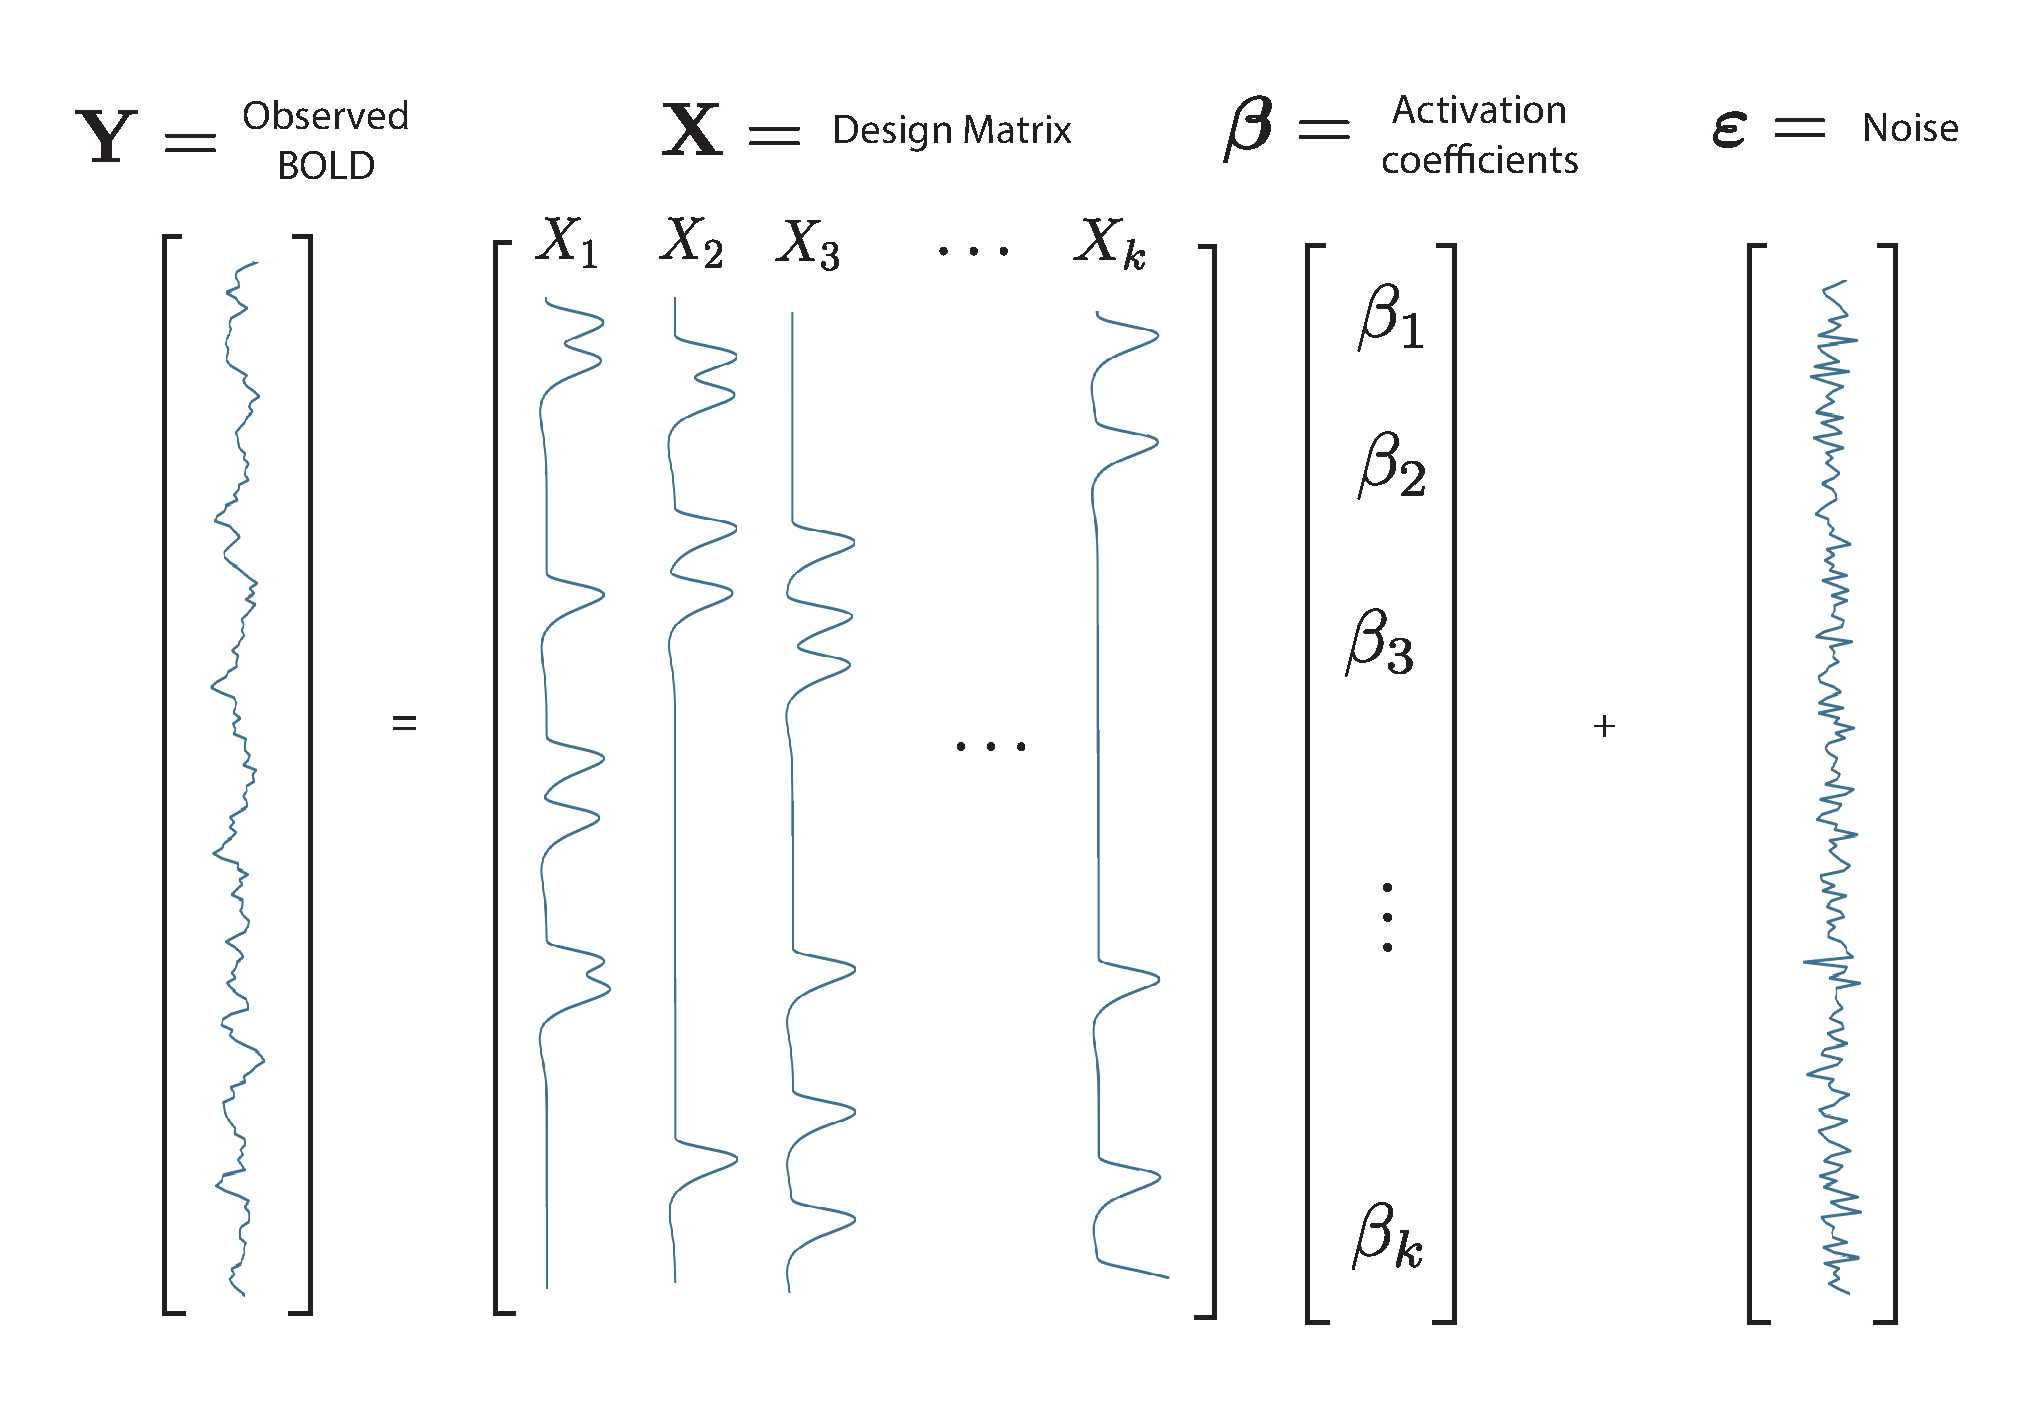
\includegraphics[width=.8\linewidth]{figures/chapter_1/glm_plain.pdf}
\caption{The GLM expresses the observed BOLD signal as a linear combination of regressors plus an error term. Each regressor of the design matrix is the convolution of a reference HRF and the stimulus function, a function that is 1 when the stimulus is present and zero otherwise. Each element of the (unknown) activation coefficients represent the relative amplitude of a given condition.}\label{fig:glm1}
\end{figure*}


Assuming Gaussian i.i.d noise, the maximum likelihood estimation of the activation coefficients is then given by $\hat{\bfbeta} = \argmin_{\bfbeta}\|\B{y} - \B{X}\bfbeta \|^2 = \B{X}^{\dagger} \B{y}$. To estimate the activation coefficients in a full brain volume this procedure is repeated independently for each voxel. Since the design matrix is the same across voxels, a matrix decomposition of $\B{X}$ such as SVD or QR can be computed once and then used to compute the least squares solution at every voxel.


In this setting we have considered the HRF to be known and fixed across the different conditions. We can easily generalize this setting to accommodate the case in which the HRF is generated by a given basis set. We will call this method \emph{basis-constrained GLM}.


\subsection{High-pass filtering and prewhitening}\label{subsec:prewhite}

The BOLD signal contains low frequency trends that are usually removed before or during the estimation of activation coefficients. One popular approach of high-pass filtering is to add a discrete cosine transform (DCT) basis set to the design matrix. When using this basis set, the highest frequency that is desired to be removed from the data has to be chosen to avoid removing the frequency of the experimental task that is also being modeled. Another approach that is becoming increasingly popular, is to fit a local regression model to the time series and remove the estimated trend from the data. The software FSL uses LOWESS (locally weighted scatterplot smoothing)~\citep{cleveland1979robust} while recent studies have successfully used a Savizky-Golay filter
\sidenote{Savitzky-Golay filter are available in Matlab under the name \texttt{\small sgolayfilt} and in Python's Scipy module under the name \texttt{\small scipy.signal.savgol\_filter}}
\citep{barry2014enhanced,ccukur2013attention}. In the studies presented in Chapter 3 we will use this last filter.  In \citep{ccukur2013attention}, the authors used a Savizky-Golay filter to estimate the low-frequency drifts with window length of 240 seconds and polynomial of degree 3. We have found that parameters close to these work well in practice. 
\newglossaryentry{AR(1)}{name={AR(1)},description={autorregressive with variance 1}}


The GLM specified in~\eqref{eq:chapter_1_glm} assumes the noise $\bvarepsilon$ follows a Gaussian random variable with covariance $\sigma^2 \B{I}$. However, it is known that the BOLD signal is temporally autocorrelated. Several authors~\citep{bullmore1996statistical,kruggel2000nonlinear} consider the BOLD noise as an autoregressive model \emph{AR(1)}. This assumes each time point is correlated with the previous time point. The distribution of the error in this case is given by $\varepsilon \sim \mathcal{N}(0, \sigma^2 \B{V})$, where $\B{V}$ is the symmetric correlation matrix and $\sigma^2$ is the variance. The correlation matrix and variance are commonly estimated from the residuals after fitting the GLM. 

The most common solution to take this special structure into account is to \emph{prewhiten} the data, that is, to remove the temporal correlation. Since the correlation matrix $\B{V}$ is symmetric and positive definite, the Cholesky decomposition can be used to find a matrix $\B{K}$ such that $\B{V}^{-1} = \B{K}^T \B{K}$. To prewhiten the data, $\B{K}$ is premultiplied on both sides of the GLM (Eq.~\eqref{eq:chapter_1_glm}) to give $\B{K}\B{y} = \B{K}\B{X} \bfbeta + \B{K}\bfvarepsilon$. This makes the errors be independent, i.e., $\B{K}\bfvarepsilon \sim \mathcal{N}(0, \sigma^2 \B{I})$.


\section{Conclusion}
In this first chapter we have presented the principal structures of the human brain. We have then presented the principal functional imaging modalities in use today, with special emphasis on functional MRI. We have seen that functional MRI is an attractive modality for functional imaging with good spatial resolution for a whole brain coverage modality. The signal measured in fMRI studies is the BOLD signal, given in the form of a succession of scans in intervals of 1-4 seconds. The extraction of time-independent activation maps from the BOLD signal relies on the linear-time-invariant property between neural response and the BOLD signal. These can be estimated by solving a least-squares problem, a setting commonly referred to in neuroimaging as the \emph{general linear model} (GLM). The GLM is usually formulated using a known form of the Hemodynamic Response Function.

\newpage

\begin{fullwidth}
\bibliographystyle{plainnat}
\bibliography{chapter_1/biblio1}
\end{fullwidth}







\chapter{Statistical Inference in fMRI}\label{chap:stats_fmri}
\markright{{~{\rm \ref{chap:stats_fmri}}. Statistical Inference in fMRI}\hfill}{}
\label{Chapter_2}



\vspace*{\fill}
\newthought{In chapter~\ref{chap:intro_fmri}}, we have presented fMRI as functional imaging modality that is non-invasive and enjoys good spatial resolution and full brain coverage. In this chapter we present the statistical methods that will be used for drawing conclusions from fMRI experiments in further chapters. 


The chapter is divided into two sections. The first section summarizes the basics of statistical hypothesis testing. We present two parametric test: the $t$-test and the $F$-test and one non-parametric test: the signed-rank Wilcoxon test. We discuss the voxel-wise parametric testing of the activation coefficients computed by the GLM. The result can be assembled into an image or map, a setting known as statistical parametric maps (SPMs).


The second section describes the basics of supervised machine learning. We introduce the supervised learning problem in the context of empirical risk minimization. We describe different surrogate loss functions and penalties that have found applications in the context of fMRI analysis. Finally, we present two applications of supervised learning to reveal cognitive mechanisms in fMRI studies. The first application is commonly known as \emph{decoding} or \emph{mind reading} and consist in predicting some information about the stimuli from the activation coefficients. The second application is known as \emph{encoding} and can be seen as the complementary operation of decoding: here, the activation coefficients are predicted from some information about the stimuli.


\hspace{20pt}
\begin{shaded}
Section~\ref{chap2_decoding} uses material from the following publication:
\begin{itemize}
\item V. Borghesani, F. Pedregosa, E. Eger, M. Buiatti, and M. Piazza, \emph{“A perceptual-to-conceptual gradient of word coding along the ventral path”} Proceedings of the 4th International Workshop on Pattern Recognition in Neuroimaging, 2014.
\end{itemize}
\end{shaded}
\vspace*{\fill}

\clearpage

\vspace*{\fill}
\minitoc
\vspace*{\fill}
\newpage

% This chapter relies on concepts from probability and measure theory that will be used without definition, such as \emph{probability space}, \emph{random variable}, \emph{population}, \emph{measurable function}, \emph{expectation}, etc. 

\section{Hypothesis testing}

A \emph{statistical hypothesis} is a statement about the parameter of a given distribution. The two complementary hypotheses in a hypothesis testing problem are called the \emph{null hypothesis} and the \emph{alternative hypothesis}. They will be denoted by $H_0$ and $H_1$, respectively. 


Given a random samples $\{x_1, \ldots, x_n\}$ drawn from a probability space $(\mathcal{X}, \mathcal{A}, P_{\theta})$, the goal of \emph{statistical hypothesis testing} is to decide, based on the random sample, whether it is possible to reject the presumed \emph{null hypothesis} $H_0$ for pre-specified level of significance. Let $\theta$ denote a distribution parameter, the general format of the null and alternative hypothesis is $H_0: \theta \in \Theta_0$ and $H_1: \theta \in \Theta_0^c$, where $\Theta_0$ is some subset of the parameter space and $\Theta_0^c$ is its complement. For example, if $\theta$ denotes the average activation of a voxel for a given condition, we might be interested in testing $H_0: \theta_0 = 0$ versus $H_1: \theta_0 \neq 0$ (or $H_1: \theta_0 > 0$).

% A \emph{hypothesis test} is a rule that specifies for which values of the sample space the decision is made to reject the null hypothesis or not. The subset of the sample space for which $H_0$ will be rejected is called the \emph{rejection region} or \emph{critical region}. Typically, given $(x_1, \ldots, x_n) \in \mathcal{X}^n$, a hypothesis test is specified in terms of a \emph{test statistic} $W(x_1, \ldots, x_n)$ = $W(\B{x})$. For example, a test might specify that $H_0$ is to be rejected if $\bar{\B{x}}$, the sample mean, is greater than 3. In this case, $W(\B{x}) = \bar{\B{x}}$ is the test statistic and the rejection region is $\{(x_1, \ldots, x_3) : \bar{\B{x}} > 3\}$.


\begin{marginfigure}
\includegraphics[width=1.\linewidth]{chapter_2/Fisher2.png}
\hspace{-20pt}\caption{Sir R. A. Fisher (London, England 1908 - Adelaide, Australia 1962) made important contributions to the field of statistics. Among many notions in statistic, he coined the terms ``test of significance'', ``Fisher consistency'' (which we will develop in Chapter 5) and ``null hypothesis''~\citep{fisher1925statistical}.}\label{fig:ronald_fisher}
\end{marginfigure}

The \emph{$p$-value} is a numerical quantity that serves to quantify the strength of the evidence against the null hypothesis and in favor of the alternative. Formally, the $p$-value is the probability of observing samples at least as favorable to the alternative hypothesis as the current samples, if the null hypothesis is true. Given a subset of the population, the $p$-value associated with a statistical test is usually computed by means of a function of these samples known as \emph{test statistic}.


Statistical tests can be broadly divided into \emph{parametric} and \emph{nonparametric} tests. Parametric test assume a known probability distribution for the distribution parameter that is under consideration. Nonparametric tests do not assume a known form of this probability distribution although they might require some regularity conditions on the distribution such as symmetry. In the following subsection we will describe two parametric statistical tests: the $t$-test and the $F$-test. In this thesis, the $t$ and $F$-test will be used to perform voxel-wise inference in section~\ref{subsec:spms}. We will also present the Wilcoxon signed-rank test, a nonparametric test that will be used to compare the performance of machine learning models in Chapter~\ref{chap:hrf_estimation} and Chapter~\ref{chap:decoding_ordinal}. The derivation of these tests is omitted but can be found in statistical textbooks such as~\citep{casella2002statistical, rice2006mathematical}.

\subsection{Parametric tests: $t$-test and $F$-test.}\label{subsec:parametric_tests}

\marginnote[-2cm]{Student was the pseudonym of Willian Sealy Gosset (England 1876 - England 1937). As a worker of the brewery Arthur Guiness \& Son he was forbidden to publish under his real name to protect the firm from its competitors. Gosset made important contributions to the field of small sample statistics. In the seminal paper \emph{The probable error of a mean}~\citep{student1908probable}, he introduced small sample estimation by means of the (Student) $t$-distribution family.}

The $t$-test is any statistical hypothesis test in which the test statistic follows a Student $t$ distribution under the null hypothesis. Most $t$-test statistics are of the form $t=Z/s$, where $Z$ and $s$ are functions of the samples, in which case the assumptions are: $Z$ follows a standard normal distribution, $s^2$ follows a $\chi^2$ distribution with $p$ degrees of freedom, and $Z, s$ are mutually independent. Once the $t$ statistic is determined, a $p$-value can be found from the values of a Student $t$ distribution with $p$ degrees of freedom.


The statistical test that has as null hypothesis that the population mean is equal to a specified value $\mu_0$ can be evaluated with a $t$-test known as the \emph{one-sample $t$-test}. Given a sample $\{x_1, \ldots, x_n\}$ of size $n$, the hypothesis
$$
H_0: \mu = \mu_0 \quad \text{versus} \quad H_1 : \mu \neq \mu_0 \quad.
$$
can be tested by performing a test that uses the test statistic
$$
t = \frac{\bar{\B{x}} - \mu_0}{ s / \sqrt{n}} \quad,
$$
where $\bar{\B{x}}$ is the sample mean, $s$ is the sample standard deviation of the sample and $n$ is the sample size. Once the test statistic $t$ has been computed, the test specifies to reject $H_0$ with significance level $\alpha$ if $t \geq t_d (1 - \alpha)$, where $t_d(1 - \alpha)$ is the $100 (1 - \alpha)$ percentile of the $t$ distribution with $d = n - 1$ degrees of freedom. 

A different test based on the $t$ distribution can be used to test the coefficients of a linear regression model. Given the equation
$$
\B{y} = \B{X}\bfbeta + b + \bfvarepsilon \quad,
$$
where $\B{X} \in \RR^{n \times p}$ is a given design matrix, $\bfbeta \in \RR^p$ and $b \in \RR$ are terms to be estimated and $\bfvarepsilon \in \RR^n$ is the error which follows a Gaussian $\mathcal{N}(0, \sigma^2 \B{I})$ distribution. It is desired to test that some linear combination of coefficients, $\B{c}^T \bfbeta$ with $\B{c} \in \RR^p$, is significantly different from zero, i.e., $H_0: \B{c}^T \bfbeta = 0 ~ H_1: \B{c}^T \bfbeta \neq 0$. In this case, the statistic
\begin{equation}
t = \frac{\mathbf{c}^T \hat{\bfbeta}}
{\hat{\sigma} \sqrt{\B{c}^T (\B{X}^T \B{X})^{-1} \B{c} }}
\label{Eq:c2_Ttest}
\end{equation}
follows a Student's distribution
with $n - (p + 1)$ degrees of freedom, where $(n, p)$ are the dimensions of the design matrix and $\hat{\sigma}^2$ is the estimate of the variance. 


The $F$-test can be seen as a generalization of the one-sample $t$-test to several groups. It can be used to asses whether the means of several pre-defined groups differ from each other. Given a total of $n$ observations, divided into $k$ groups of samples $\B{x}_1, \ldots, \B{x}_k$ with respective sizes $n_1, \ldots n_k$, a null hypothesis is of the form
$$
H_0 : \mu_1 = \mu_2 = \cdots = \mu_k \quad \text{versus} \quad H_1 : \text{at least one} ~\mu_i \neq \mu_j \quad,
$$
then the test statistic to test this hypothesis is calculated as the ratio between the between-group variability and the within-group variability:
\begin{equation}\label{eq:t_test}
F = \frac{\sum_i n_i (\bar{\B{x}}_i - \bar{\B{x}})^2 / (k-1)}{\sum_{ij} (\B{x}_{ij} - \bar{\B{x}}_i)^2 / (n - k)}.
\end{equation}

This statistic follows the $F$-distribution (also known as Snedecor's $F$ distribution or the Fisher–Snedecor distribution) with $(k-1, n-k)$ degrees of freedom under the null hypothesis, i.e. the null hypothesis can be rejected according to this test with significance level $\alpha$ if the F statistic is greater than $F_{(k-1, n-k)}(1 - \alpha)$, where $F_{(k-1, n-k)}$ denotes the $F$-distribution with $(k-1, n-k)$ degrees of freedom.

{As done previously for the $t$-test, a variant of the $F$-test can be used to test the coefficients of a linear regression model. In this case, instead of testing that a given contrast is significantly different from zero, we will test that a \emph{set of contrasts} are all simultaneously different from zero. In this case the contrast $\B{C}$ is a matrix with $k$ columns describing the possible linear combinations to be tested. For example, using a model with four parameters, to test whether all of them are equal to $0$, $H_0: \beta_1 = \beta_2 = \beta_3 = \beta_4 = 0$, one would specify a contrast of the form $\B{C} = \B{I}$, where $\B{I}$ is the identity matrix of size $4 \times 4$.

For an arbitrary contrast $\B{C}$, the $F$-statistic for this test is given by
$$
F = \frac{\text{Tr}(\B{C}\bfbeta \bfbeta^T \B{C}^T)}{
\hat{\sigma}^2 \text{Tr}({\B{C}^T (\B{X}^T\B{X})^{-1}\B{C}}) \quad,
}
$$
where the square root is taken element-wise. This expression follows an $F$ distribution with $r$ numerator and ${n - (p+1)}$ denominator degrees of freedom ($F_{r, n - (p+1)}$), where $r$ is the rank of $\B{C}$.
}

\subsection{Nonparametric tests: Wilcoxon signed-rank test.}\label{subsec:wilcoxon}


The \emph{Wilcoxon signed-rank} test can be used to asses whether two population means differ. That is, given the samples $\{x_1, \ldots, x_n\}$ and $\{y_1, \ldots, y_n\}$, we would like to test the following hypothesis $H_0: \bar{\B{x}} = \bar{\B{y}}, ~~ H_1: \bar{\B{x}} \neq \bar{\B{y}}$, where $\bar{\B{x}}$ is the sample mean, $\bar{\B{x}} = \frac{1}{n}\sum_{i=1}^n x_i$.


Because of this, it can be seen as a nonparametric alternative to the two-sample $t$-test. We will use the Wilcoxon signed-rank test to replace the two-sample $t$-test when the normality assumptions of the last are not met. The assumptions behind Wilcoxon signed-rank are that \emph{(a)} the two samples are paired (paired samples imply that each individual observation of one sample has a unique corresponding member in the other sample), and \emph{(b)} the distribution of the difference between the values within each pair must be symmetrical, i.e., the median difference must be identical to the mean difference. Beginning with a set of paired values $\B{x}_1$ and $\B{x}_2$, each of size $n$, the test statistic $W$ can be computed following the steps:
\begin{itemize}
\item calculate $|{x}_{1, i} - {x}_{2, i}|$ and $\text{sign}({x}_{1, i} - {x}_{2, i})$ for every $1 \geq i \geq n$. Exclude pairs which have zero difference.
\item order the remaining $n_r$ pairs from smallest absolute difference to largest absolute difference $|{x}_{1, i} - {x}_{2, i}|$.
\item rank the pairs, starting with the smallest as 1. Ties receive a rank equal to the average of the ranks they span. Let $r_i$ denote the rank.
\item calculate the test statistic $W = |\sum_{i=1}^{n_r} \text{sgn}({x}_{1, i} - {x}_{2, i}) r_i|$
\end{itemize}

As $n_r$ increases, the distribution of $W$ converges to a normal distribution. For small samples ($n_r < 10$), $W$ is compared to a critical value from a reference table.

%
% \subsection{Likelihood Ratio Tests}

% For a given hypothesis, different tests can be derived. The Neymann-Pearson lemma shows that the likelihood-ratio test is optimal.

% The \emph{likelihood ratio test} is a statistical test for making a decision between the null and alternative hypothesis based on the value of this ratio. Given a likelihood function $L(\theta|\beta)$ which is a function of the parameter $\theta$ with $\beta$ held fixed at the value that was actually observed, we defined the \emph{likelihood ratio} as
% $$
% \Lambda = \frac{ \sup\{ L( \theta | \bfbeta) : \theta \in \Theta_0 \}}{\sup\{ L(\theta | \bfbeta) : \theta \in \Theta \} }
% $$

% The likelihood ratio test rejects the null hypothesis $H_0$ when its inverse exceeds a critical value $\lambda_{\alpha}$. That is, the decision rule has the form:
% \begin{itemize}
% \item if $\Lambda^{-1} \geq \lambda_{\alpha}$~ reject $H_0$
% \item if $\Lambda^{-1} \geq \lambda_{\alpha}$~ do not reject $H_0$.
% \end{itemize}

% The rationale behind the 

% The critical value $\lambda_{\alpha}$ is usually chosen to obtain a specific significance level $\alpha$, through the relation $P_0(\Lambda \geq \lambda_{\alpha}) = \alpha$, where $P_0$ denotes the probability under the null hypothesis. The Neyman-Pearson lemma states that this likelihood ratio test is the most powerful among all level-$\alpha$ tests for this problem. The value of $\alpha$ is called the \emph{$p$-value} associated with the observation $\lambda_{\alpha}$ under the null hypothesis, and represents the chance under the null hypothesis of observing a test statistic $\lambda_{\alpha}$ as large or larger than actually observed.


% \begin{itemize}
% \item {\bf One-sample t-test}. In testing
% \end{itemize}



\subsection{Voxel-wise hypothesis testing: Statistical Parametric Maps} \label{subsec:spms}




Statistical Parametric Maps (SPMs)\sidenote{Statistical Parametric Mapping (SPM) can refer both to the set of techniques detailed in this section and to the SPM software distributed by the \emph{Wellcome Department of Imaging NeuroScience} at University College London.} are images with values that are, under the null hypothesis, distributed according to a known probability density function, usually Student $t$ or the $F$ distribution. To create such maps, one proceeds by performing a parametric test at each voxel. The resulting statistics are assembled into an image - the SPM. 

Given the activation coefficients for a single voxel $\beta \in \RR^k$ (cf. Section~\ref{chapter_1_GLM}), with $k$ being the number of conditions, it is possible to use a $t$-test to test whether  a given linear combination of the conditions is significantly different from zero. As we did in section~\ref{subsec:parametric_tests} we introduce the contrast $\mathbf{c}\in \RR^k$ so that $\mathbf{c}^T \bfbeta$ is a linear combination of the conditions. The hypothesis can then be written as $H_0: \B{c}^T \bfbeta = 0$, $H_1: \B{c}^T \bfbeta \neq 0$. In this case, under the assumptions of the $t$-test for the coefficients of a linear regression model (Gaussian and i.i.d noise in the \gls{GLM}), equation~\ref{eq:t_test} gives the expression of the statistic for this test. Assigning the statistic to every voxel creates an image with the same dimensions as the input brain images, in this case a the image is called a $t$-map because of the $t$-test used to generate it.


\begin{figure}
\begin{center}
\includegraphics[width=.8\linewidth]{chapter_2/spm_visual_auditory.pdf}
\end{center}
% \vspace{-4ex}
\caption{$t$-map for a contrast of a Visual vs an Auditory task. Thresholded at $p$-value $< 10 ^ {-3}$. It can be seen how the voxels that exhibit a higher significance of this contrast belong to visual areas (red) and auditory areas (blue).}\label{fig:t_test_localizer}
\end{figure}


Figure~\ref{fig:t_test_localizer} plots the $t$-map resulted from a functional localizer~\citep{pinel2007fast} performed as part of the acquisition in~\citet{borghesani:hal-00986606} dataset. For this, the conditions `Visual' and `Auditory' were compared. Since only two conditions were compared, the contrast is of the form $\B{c} = [+1, -1, 0, \ldots, 0]$ where the entry $+1$ is for the Visual condition and $-1$ for the auditory condition. The image is thresholded so that only voxels with a $p$-value smaller than $10^ {-3}$ are displayed. It can be seen how the voxels that exhibit a higher significance of this contrast belong to visual areas (red) and auditory areas (blue) [see Figure~\ref{fig:chapter_1_functions} for a localization of some brain regions]. This example involves the testing of a single contrasts using a $t$-statistic. In similar fashion, the test in which we consider $d$ contrasts, i.e. $H_0: \B{c}_1^T \bfbeta$ = $\B{c}_2^T \bfbeta$ = $\cdots$ = $\B{c}_d^T \bfbeta$ = 0 and $H_1:$ at least one $\B{c}_i^T\bfbeta \neq 0$ can be performed using an $F$-test as described in section~\ref{subsec:parametric_tests}.



% \subsection{Permutations testing}

% {\blue 
% Discuss parametric and nonparametric. \citep{nichols2002nonparametric, goodpermutation} and Polina for the classification side. 
% % Stuff in here http://www2.warwick.ac.uk/fac/sci/statistics/staff/academic-research/nichols/software/snpm/#Refs
% }


% In order to perform hypothesis testing, we need to know the probability distribution of the selected statistic under the null hypothesis. For example, the previously mentioned $t$-test assumes the probability density of the statistic is the Student distribution. However, deriving a parametric distribution for a particular statistic requires making strong assumptions on the generative model of the data. Consequently, nonparametric techniques, such as \emph{permutation tests}~\citep{goodpermutation}, can be of great value if the distribution of the data is unknown.


% Permutation testing can be traced back to at least Fisher (XXX 1935, Chapter 3). Instead of comparing the actual value of a test statistic to a standard statistical distribution, the reference distribution is generated from the data themselves, as described below. 

% {\blue Good reference~\citep{golland2003permutation}}

% the theoretical distribution of the test statistic may only be known under particular assumptions that may be be violated in practice. The specificity of the test is then impacted. Alternatively, one may want to use a specificc test statistic, the theoretical distribution of which is not known under the null hypothesis. This is likely to happen for computational reasons for instance. The Monte-Carlo method [33] can be used to empirically approximate the unknown distribution: N artificial datasets are created on the model of the original data under the null hypothesis, so that N realizations of the test statistic are observed. However, it is difficult to reproduce the real-data problem with simulations. Permutation testing can be seen as a way to build the unknown H0 distribution from the observed data. Those are transformed in such a way the decision statistics' distribution remains the same under the null hypothesis, 


\subsection{Multiple comparisons issues}




One major drawback of statistical parametric maps is the multiple comparisons issue. This occurs when multiple hypothesis tests are performed simultaneously and one must account for the possibility of errors occurring on each of these tests~\citep{toothaker1993multiple, miller1966simultaneous, westfall1993resampling}. In fMRI, due to the huge amount of voxels (on the order of $4 \times 10^4$ at $3mm^3$ resolution), some tests can lead to a large amount of false positive results, i.e., some voxels are found to be significant while in reality they were not. As a result, it is necessary to consider other types of error rates which account for the multiple comparisons issue. 

A simple procedure to control the rate of false positives is through the \emph{Bonferroni correction} method. This approach consists in dividing the threshold $\alpha$ by the number
of tests $p$, which yields the new threshold $\alpha_b = \alpha / p$.
%  Indeed, in order to have a global test (brain-wide test) with a significance
% level of $\alpha$ (\emph{i.e.} a probability of incorrectly rejecting the null
% hypothesis of $\alpha$), the different tests (voxel-wide tests) have to be
% performed with a very low significance level $\alpha/p$, where $p$ is the
% number
% of unitary tests.
The maps of voxels selected by thresholding the \emph{$p$-values} for the object
recognition task (subject 1), are given in Fig.\ref{fig:chapter_2_comparisons},
for different threshold values ($0.05$, $0.01$ and $0.05$ corrected by
\emph{Bonferroni}).
We notice that \emph{Bonferroni correction} is very severe, and that
it keeps very few significant voxels. 

\begin{figure}
\begin{center}
\includegraphics[width=.8\linewidth]{chapter_2/spm_visual_auditory_pval005.pdf}
\includegraphics[width=.8\linewidth]{chapter_2/spm_visual_auditory_pval001.pdf}
\includegraphics[width=.8\linewidth]{chapter_2/spm_visual_auditory_pval005_corrected.pdf}
\end{center}
% \vspace{-4ex}
\caption{\emph{Visual vs Auditory contrast}. Visualization of the voxels selected by
thresholding the
\emph{$p$-values} for the Visual vs Auditory contrast at different thresholds
($0.05$, $0.01$ and $0.05$ corrected by \emph{Bonferroni}). The \emph{Bonferroni
correction} is very severe and keeps very few voxels.
}\label{fig:chapter_2_comparisons}
\end{figure}


One of the main limitations behind Bonferroni corrections is that it does not take into account the spatial structure of the SPM. As such the number of independent test can smaller than the number of voxels. 
% Because of this, Bonferroni correction is widely regarded as being too conservative.
Other approaches besides Bonferroni correction include random field theory~\citep{friston1994assessing, worsley1992three} and resampling techniques~\citep{Friman2005859, holmes2003bootstrapping}. The review papers~\citep{Logan200495, Nichols2012811} provide an overview of the different methods that have been proposed to overcome this problem.



\section{Machine learning in fMRI}

\newglossaryentry{decoding}{name=decoding,description=distinguish patterns of neural activity associated with different stimuli or cognitive states}
\newglossaryentry{encoding}{name=encoding,description=predicting patterns of brain response to novel stimuli based on their features}


While classical statistical modeling emphasizes statistical inference (confidence intervals, hypothesis test, optimal estimators), the field of \emph{machine learning}, also known as statistical learning and pattern recognition, emphasizes model validation as measured by its performance on unseen samples. That is, in machine learning the validity of an estimated model will be judged based on its generalization performance. 

The first applications of machine learning to neuroimaging focused on distinguishing patterns of neural activity associated with different stimuli or cognitive states, a problem commonly known as \emph{\gls{decoding}}, \emph{reverse inference} or \emph{brain reading}~\citep{dehaene1998inferring, cox2003,laconte2005support, thirion2006, Sutao2011} uses a machine learning model to discriminate patterns of neural activity associated with different stimuli or cognitive states. In this thesis we will also  describe the~\emph{encoding} problem~\citep{thirion2006, Kay2008, mitchell2008predicting}, in which the patterns of brain activity are predicted based on the stimuli features. Encoding and decoding can be seen as complementary operations: encoding uses stimuli to predict activity while decoding uses activity to predict information about the stimuli. We will further describe these settings in Section~\ref{chap2_decoding} and \ref{chap2_encoding}, respectively.


% {\blue In this thesis we focus on supervised learning models, i.e. models in which the training set contains samples and labels. Other machine learning settings include unsupervised learning (where the training labels are not available), semisupervised learning (where only a fraction of the training labels are available) and reinforcement learning (where a fraction of the training samples and its respective target values are obtained during the learning process). The models that we will use in this thesis will belong to the supervised learning setting }.



% The shift from univariate methods to multivariate methods also entails a change in the questions that can be asked to fMRI studies. While univariate methods ask the question of which regions of the brain which are more active for one condition compared to another, multivariate methods can ask what information is represented in a region in terms of brain states associated with distinct patterns of activity, and how that information is encoded and organized~\citep{Haxby2012}.

\subsection{Supervised Learning}\label{subsec:supervised_learning}

Supervised learning is the task of learning a function from labeled training data. We will now give a formal definition of the task. 

We consider two spaces $\mathcal{X}$ and $\mathcal{Y}$. We will refer to $\mathcal{X}$ as the \emph{sample space} and to $\mathcal{Y}$ as the \emph{target space}. We assume that the pair $(X, Y)$ is a random variable taking values in $\mathcal{X} \times \mathcal{Y}$ and distributed according to an \emph{unknown} probability distribution $P$.  We observe a sequence of $n$ i.i.d. pairs  $\{(x_1, y_1), \ldots, (x_n, y_n)\} \in (\mathcal{X} \times \mathcal{Y})^n$ sampled according to $P$ and the goal is to construct  a function $h: \mathcal{X} \to \mathcal{Y}$ which \emph{predicts} $Y$ from $X$.

We need a criterion to choose this function $h$. For this we are given a \emph{loss function} $\ell: \mathcal{Y} \times \mathcal{Y} \to \RR$ that measures the disagreement between a pair of elements in the target space. This way $\ell(y_i, f(x_i))$ quantifies the penalty of predicting the target $f(x_i)$ when the true label is $y_i$. The objective is to construct a function $h$ such that its \emph{risk} is as small as possible. The risk of a function $h$ is defined as:
$$
\mathcal{R}(h) = \mathbb{E}_{X \times Y}(\ell(Y, h(X)))
$$

A function that achieves the minimum risk over all possible measurable functions is called the \emph{Bayes predictor} and is denoted $h^*$:
$$
h^* \in \argmin_h \mathcal{R}(h)
$$



However, in general the risk cannot be computed because the distribution $P$ is unknown. As an alternative we can use an approximation of the risk, called the~\emph{empirical risk}, by averaging the loss function over the pairs $\{(x_1, y_1), \ldots, (x_m, y_m)\} \in (\mathcal{X} \times \mathcal{Y})^m$ drawn from $P$. The empirical risk is defined as: 
\begin{equation}\label{eq:empirical_risk}
{{\mathcal{R}}_n}(f) = \frac{1}{n} \sum_{i=1}^n \ell(y_i, f(x_i)) \quad.
\end{equation}

% {\blue In this case the $n$ elements $\{X_1, X_2, \ldots, X_n\}$ in the training set can be represented as a $n \times p$ matrix, $\B{X} \in \RR^{n \times p}$ and the $n$ target elements from the training set $\{y_1, y_2, \ldots, y_n\}$ can be represented as a vector $\B{y} \in \RR^n$.}

\begin{marginfigure}
\includegraphics[width=\linewidth]{chapter_2/vc.png}
\caption{Vapnik–Chervonenkis theory (also known as VC theory) was developed during 1960–1990 by Vladimir Vapnik (right) and Alexey Chervonenkis (left). The theory attempts to explain the learning process from a statistical point of view.}
\end{marginfigure}

The task is then to find the function $f$ that minimizes the empirical risk, a setting known as \emph{empirical risk minimization}~\citep{vapnik1974teoriya}. Although the methods studied in this thesis can be seen within the framework of empirical risk minimization, several alternatives exist to this framework. A different setting for the estimation of learning models is \emph{maximum likelihood estimation}, in which the model parameters are chosen as the maximizers of the likelihood function. When the loss function $\ell$ can be written as the negative log likelihood: $\ell(y, f(x)) = -\log P(f(x)|x)$, then empirical risk minimization is equivalent to maximum likelihood estimation.

\paragraph{Classification.} If the target space $\mathcal{Y}$ is a finite set then the learning problem is known as \emph{classification}. In the special case that this target space contains only two different values, then this problem is known as \emph{binary classification}. The common loss $\ell$ in this setting is the zer-one loss, defined as $\ell(y, \hat{y}) = 0$ if $y = \hat{y}$ and $0$ otherwise.

\paragraph{Regression.} If on the other hand the target space is identified with an interval of $\RR$ we speak about a \emph{regression} problem. For example, the task of predicting the gender of a person would be a (binary) classification task since only two outcomes are possible. On the other hand, the task of predicting the height of a person is considered a regression task since the target space is an interval from the real line. The encoding and decoding problems in fMRI that we will consider in this chapter can be framed either using classification or regression models. The \emph{pairwise ranking} and \emph{ordinal regression} models that we will consider in Chapter~\ref{chap:decoding_ordinal} and \ref{chap:consistency} can be seen as a special case of classification problems in which the loss function depends on the distance between the respective labels. As we will see in Chapter~\ref{chap:decoding_ordinal}, one of the contributions of this thesis is to show that certain decoding problems can be formulated using ranking and ordinal regression models rather than multiclass or regression. 

For most practical applications, the sample space $\mathcal{X}$ is identified with $\RR^p$, where $p$ is referred to as the \emph{dimensionality} or \emph{number of features} of the learning problem and the target space $\mathcal{Y}$ is identified with $\RR$.




\subsection{Surrogate loss functions.}\label{subsec:surrogate_loss_functions}

\begin{marginfigure}[2cm]
\hspace{-20pt}\includegraphics[width=1.2\linewidth]{chapter_2/loss_01.png}
\vspace{-10pt}\caption{
	The direct minimization of the empirical risk for the 0-1 loss is a difficult computational problem due to the discontinuity of and non-convexity of the loss function. In the figure: plot of the surface $g(w_1, w_2) = \mathcal{R}(f)$, where $f$ is the linear classification function $f(\B{x}) = \sign(\B{x}^T \B{w})$ with $\B{X} \in \RR^{10 \times 2}$ a random normally distributed matrix.
	This surface is discontinuous with large, flat regions and is thus not amenable for optimization using gradient-based methods.
}\label{fig:01_minimization}
\end{marginfigure}

\newglossaryentry{Heaviside}{name=Heaviside,description=The real function that is zero for negative values and one otherwise}


The direct minimization of the empirical risk is often not a tractable optimization problem. For example, consider the binary classification 0-1 loss, defined as
$$
\ell_{0-1}(y, \hat{y}) = \mathcal{H}( - y \cdot \hat{y}) \quad,
$$
where $\mathcal{H}$ is the \gls{Heaviside} step function, defined as $\mathcal{H}(x) = 1$ if $x \geq 0$ and $0$ otherwise.
Minimization of the empirical risk associated with this loss is known to be NP-hard even for the class of functions as linear classifiers. See Figure~\ref{fig:01_minimization} for an informal justification and \citep{feldman2012agnostic} and reference therein for a formal discussion of these properties. 

For this reason it is common to consider instead a function ${\psi: \mathcal{Y} \times \RR^d \to \RR}$ which is an approximation to the true loss known as \emph{surrogate loss} function. $d$ is an integer that will be determined by the surrogate loss function. For binary classification, $d$ is usually 1, while for multiclass classification $d$ is usually equal to the number of classes. The goal in this setting is to minimize the empirical $\psi$-risk, defined as
$$
{\mathcal{R}}_{n}^{\psi}(g) = \frac{1}{n} \sum_{i=1}^n \psi(y_i, g(x_i)) \quad.
$$
For computational reasons, $\psi$ is often a convex function in its second variable (the variable with respect to which we will minimize). Note that in this case the function $g$ has as output space $\RR$ and not $\mathcal{Y}$ as was the case before, thus the function $g$ is not a prediction function. In binary-class classification, the prediction of two classes is given by the sign of this function. In this case, we will call $g$ a decision function and $\text{sign}(g(X))$ will be the prediction function while in multiclass classification the prediction function is usually given by $\argmax_{c \in \{1, \ldots, k\}} g_i(x)$ \citep{Zhang2004}.


Compared to the empirical risk minimization setting, we have replaced the original problem by one with better computational properties. It is natural to ask whether what have we lost in the process. In Chapter~\ref{chap:consistency} we will present results on the consistency of surrogate loss functions, that is, under which conditions minimizing the $\psi$-risk leads to the same solution as minimizing the risk. There, we will review existing results for binary classification and prove novel results for the case of ordinal regression.



The following is a list of surrogate loss function that are commonly used in the context of encoding and decoding models. As classification models we will consider Support Vector Machines (SVM) and Logistic Regression. For simplicity we will only describe binary classification models and assume the target space consists only of the labels $\mathcal{Y} = \{-1, 1\}$. Several techniques exist to convert a binary classification model into a multiclass classification model, such as one-vs-all and one-vs-rest~\citep{bishop2006pattern}. As regression models we will mention Support Vector Regression and Least Squares. Pairwise ranking and ordinal regression models will be described in Chapter~\ref{chap:decoding_ordinal} and \ref{chap:consistency}. 

Let $y \in \mathcal{Y}$ and $\alpha \in \RR$, then the surrogate loss functions are defined as:

% \begin{marginfigure}
% {\vspace{-20pt}\hspace*{-20pt}\includegraphics[width=1.3\linewidth]{chapter_2/decision_func_0.pdf}
% \vspace{-20pt}\hspace*{-20pt}\includegraphics[width=1.3\linewidth]{chapter_2/decision_func_1.pdf}}
% \caption{Example of linear prediction function and non-linear prediction function on a binary classification problem. The classifier will classify all the points on one side of the decision boundary (denoted here with a black line) as belonging to one class and all those on the other side as belonging to the other class. For linear decision functions, the decision surface is an affine function.
% Up: linear SVM showing an affine decision boundary. Down: SVM with polynomial degree 3 kernel, showing a non-linear decision boundary}
% \end{marginfigure}


\begin{marginfigure}
\includegraphics[width=\linewidth]{chapter_2/losses_color.pdf}
\caption{Different surrogate loss functions presented in the text (for y=1): hinge loss, logistic loss and squared loss}
\end{marginfigure}

\newglossaryentry{hinge loss}{name=hinge loss,description=Loss function used by Support Vector Machines}

\begin{itemize}
\item {\it Support Vector Machines (SVM)}. Since its first use in decoding models by~\citet{cox2003}, Support Vector Machines~\citep{Boser:1992:TAO:130385.130401, cortes1995support} have become the reference approach for classification decoding studies. Its success comes from its availability in popular software packages, its overall good performance under a wide array of circumstances~\citep{bottou1994comparison, king1995statlog, caruana2006empirical} and its ability to cope with high-dimensional data. The following surrogate is known as the \emph{\gls{hinge loss}},
\begin{equation} \label{eq:hinge}
\psi(y, \alpha) = \text{max}(1 - y \alpha, 0) \quad .
\end{equation}
Support Vector Machines can be extended to non-linear decision functions through the use of \emph{kernels}~\citep{shawe2004kernel}.


\marginnote{``In the terminology of statistics, this model is known as logistic regression, although it should be emphasized that this is a model for classification rather than regression.'', Christopher M. Bishop (2006). \emph{Pattern Recognition and Machine Learning}.p. 205. }
\item {\it Logistic Regression}. Logistic Regression is a classification model that models the posterior probability as a sigmoid, that is, $P(y|X)$ = $(1 + e^{- y f(X)})^{-1}$. This allows to provide the probability estimates for class membership. The surrogate loss function in this case is given by the negative log-likelihood, that is, also known as the \emph{logistic loss}
\begin{equation}\label{eq:logistic_loss}
\psi(y, \alpha) = \log(1 + \exp({y}\alpha)) ~\quad.
\end{equation}

\item {\it Support Vector Regression}. This is a variant of Support Vector Classification for the regression setting proposed by~\citep{drucker1997support}. The surrogate loss function in this case is known as the \emph{$\varepsilon$-insensitive loss} and is given by
\begin{equation}\label{eq:svr}
\psi(y, \alpha) = \text{max}(|y - \alpha| - \varepsilon, 0) \quad ,
\end{equation}
where $\varepsilon > 0$.


\item {\it Least Squares} is a regression model that minimizes the square of the distance to the prediction. The loss function is given by 
\begin{equation}\label{eq:least_squares}
\psi(y, \alpha) = (y - \alpha)^2 \quad.
\end{equation}
% The values of $\B{w}, c$ that minimize this loss can be computed in closed form as
% $$
% [\hat{\B{w}},~\hat{c}] = \tilde{\B{X}}^{\dagger}\B{y} \quad,
% $$
% where $\tilde{\B{X}}$ is the matrix formed by stacking a column of ones to the original design matrix $\B{X}$.
\end{itemize}


The most popular choice for prediction functions in encoding and decoding models are linear decision functions~\citep{cox2003,laconte2005support, Sutao2011, thirion2006, Naselaris2011}, that is, functions of the form $f(\B{x}) = \text{sgn}(\B{x}^T \B{w} + c)$ for a binary classification problem and $f(\B{x}) = \B{x}^T \B{w} + c$ for a regression problem, where $\B{w} \in \RR^p$ and $c \in \RR$ are unknown parameters to be estimated. 

% These methods assume a linear relationship between the samples and the target variable. We will see in Chapter 5 that pairwise ranking and ordinal regression models can capture a certain degree of non-linearity between the samples and the target variable while maintaining most of the advantages of linear models~\citep{pedregosa:hal-00717990, Doyle2013}.



% It has been found that linear models often outperform non-linear models in the context of decoding \citep{cox2003,laconte2005support, Sutao2011} and encoding studies~\citep{thirion2006, Naselaris2011}.
% However, this supposed superiority can be due to
% an intrinsic linear relationship between the neural
% coding and the cognitive target or simply because the non-linear prediction functions used have not been able to capture the
% true non-linearity of this relationship (e.g. due to lack of training data). 



\subsection{Regularization}\label{subsec:regularization}

Regularization has long played a fundamental role in statistics and related mathematical fields. First introduced by~\citet{tikhonov1977solutions} in the context of solving ill-posed integral equations, it has since become a standard part of the statistical toolkit. 


\begin{marginfigure}
\vspace{10pt}\hspace{-10pt}\includegraphics[width=1.\linewidth]{chapter_2/regularization.pdf}
\caption{ The machine learning models that we will consider are estimated as the minimization of a \colorbox{color2}{trade-off} between \colorbox{color1}{data fidelity} and a \colorbox{color3}{regularization} term. Regularization is used to bias the estimated model towards a set of desired solutions.}\label{fig:regularization_formula}
\end{marginfigure}


The purpose of regularization is to use prior knowledge of the problem to bias the estimated model. This can be desirable to solve an ill-posed problem or to avoid overfitting. In this setting, the model is estimated as a solution to an optimization problem of the form
$$
\argmin_{f \in \mathcal{F}} {\mathcal{R}}_n^{\psi}(f) + \lambda \Omega(f) \quad,
$$
where $\Omega(f)$ is the \emph{regularization}, which biases solutions toward a desired kind of solutions and $\mathcal{F}$ is a family of functions (e.g. the family of linear or polynomial functions). In this setting the parameter $\lambda$ controls the trade-off between data-fidelity and the regularization term.

We will present the following penalties due to their widespread use in fMRI analysis. These assume a linear decision function $f$, i.e., $f(\B{x}) = \B{w}^T \B{x} + c$ or $f(\B{x}) = \sign(\B{w}^T \B{x} + c)$ and the penalty will be expressed in terms of the parameters $\B{w}$.


\begin{itemize}

\item {\it squared $\ell_2$} $\left(\Omega(\B{w}) = \|\B{w}\|^2_2 \right)$ . Equivalent to Gaussian normal prior with zero mean~\citep[Chapter 3]{bishop2006pattern}. When loss is linear least squares, it is referred to as Ridge regression and the estimated model $(\hat{\B{w}}, \hat{c})$ has the closed form solution for $\lambda > 0$:
$$
[\hat{\B{w}},~\hat{c}] = (\tilde{\B{X}}^T \tilde{\B{X}} + \lambda n \tilde{\B{I}})^{-1} \tilde{\B{X}}^T \B{y} \quad,
$$
where $\tilde{\B{X}}$ is the matrix formed by stacking a column of ones to the original design matrix $\B{X}$ and $\tilde{\B{I}}$ is the diagonal matrix with all ones except a zero in the last diagonal element, i.e. $\tilde{\B{I}} = \B{I} - \B{e}_n \B{e}_n^T$. This penalty is sometimes also used for computational reasons since it makes the optimization problem better conditioned.

\item {\it $\ell_1$ regularization} $\left(\Omega(\B{w}) = \|\B{w}\|_1 \right)$. Promotes~\emph{sparse} solutions, i.e. solutions with a large fraction of zero coefficients. When combined with a least squares loss function, the model is known as \emph{lasso}~\citep{tibshirani1996regression} and \emph{basis pursuit denoising}~\citep{chen2001atomic}. 

\item {\it elastic-net regularization} $\left(\Omega(\B{w}) = \alpha \|\B{w}\|_1 + (1 - \alpha) \|\B{w}\|^2_2 \right)$. Linearly combines $\ell_1$ and squared $\ell_2$ regularization. In the case of severely correlated variables, the $\ell_1$ penalty tends to select one variable from the group of highly correlated variables and ignore the rest. To mitigate this problem, elastic-net penalty adds a quadratic $\ell_2$ norm to the penalty~\citep{Zou05regularizationand}.

\item {\it total variation (TV)}~\citep{rudin1992nonlinear, chan1999nonlinear, michel2011total}. Total-variation, defined as the $\ell_1$ norm of the gradient promotes piecewise constant solutions. It can be combined with $\ell_1$~\citep{baldassarre2012structured, gramfort:hal-00839984, dohmatob:hal-00991743} and with elastic-net~\citep{dubois2014predictive} penalties. Figure~\ref{fig:tv_reg} compares the estimated coefficients by the use of elastic-net and TV+$\ell_1$ regularization.

% \item {\it nuclear norm regularization} $\left(\Omega(\B{w}) = \|\B{W}\|_* \right)$. This is defined on a matrix.
\end{itemize}

\begin{figure}
\includegraphics[width=1.07\linewidth]{chapter_2/regularization_gramfort.pdf}
\caption{Regularization biases the estimated model towards a desired set of solution. 
In this figure we show the estimated coefficients of a linear model with different regularizations. 
In this model the estimated coefficients correspond to voxels in a brain volume and are displayed over an anatomical image.
In the left, elastic-net regularization yields sparse although very scattered coefficients. Moreover, this regularizer does not take into account the spatial structure of the image. The TV+$\ell_1$ regularization in contrasts yields blobs of nonzero coefficients surrounded zero elements. This latter model has been proved to yield predictive regions which are meaningful from a cognitive point of view. Source: adapted from~\citep{gramfort:hal-00839984}.}\label{fig:tv_reg}
\end{figure}


\vspace{20pt}





\subsection{Model evaluation and cross-validation.}


Since it is possible to construct a classifier that predicts perfectly on the train set but with very poor generalization performance (e.g. the classifier that returns the right label for a sample it has already seen and random otherwise), computing the empirical error on the training set yields a very poor estimator of the true risk of a model.


Cross-validation is a technique to iteratively partition the input dataset in order to obtain a more reliable estimator of the risk~\citep{mosteller1968data, stone1977asymptotics, geisser1975predictive, arlot2010survey}. In this setting a subset of the data is used for training (the \emph{training set}) and the rest of the data is used to compute the accuracy of the trained model (the \emph{test set} or \emph{validation set}). Repeating the process several times and averaging the accuracy of the predictions across the validation sets yields an estimator of the risk. One form of cross-validation leaves out a single observation at a time; this is known as leave-one-out. Another form, known as K-fold cross-validation, splits the data into K subsets; each is held out in turn as the validation set.



The cross-validation score is the average of the empirical risk across all the folds, which is itself an estimator of the risk. This can then be used to perform hypothesis relative to the risk of two predictors $f$ and $g$. For example, consider the test in which we compare the risk of two estimators, that is, $H_0: \mathcal{R}(f) = \mathcal{R}(g)$ and $H_1: \mathcal{R}(f) \neq \mathcal{R}(g)$. This statistical test can be performed using the Wilcoxon signed-rank test presented in Section~\ref{subsec:wilcoxon}. This test takes as input two sequences 
%$\{a_1, \ldots, a_n\}$ and $\{b_1,\ldots, b_n\}$, 
in which the samples are the empirical risk at the different cross-validation folds.

\begin{marginfigure}
\hspace{-10pt}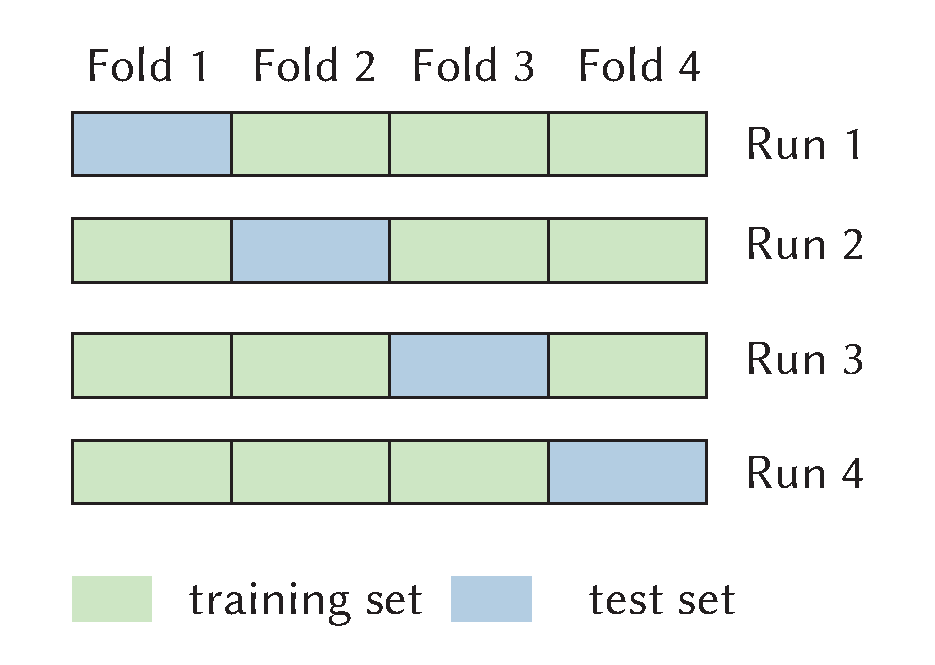
\includegraphics[width=1.2\linewidth]{chapter_2/runs_cv.pdf}
\caption{
	The technique of $K$-Fold cross-validation, illustrated here for the case $K = 4$, involves taking the available data and partitioning it into $K$ groups. Then $K-1$ groups are used (in green) to train a set of models that are then evaluated on the remaining group (in blue). 
}\label{fig:k_fold_cv}
\end{marginfigure}
Cross-validation is an attractive estimator of the risk since it makes no assumptions on the model or the loss function. Alternatives exist for specific loss functions such as Stein's unbiased risk estimate~\citep{stein1981estimation, donoho1995adapting} which is an unbiased estimator of the mean-squared error.

Cross-validation can be used to select the regularization parameter in a setting known as \emph{nested cross-validation}. In this setting, the train set is again split into the different cross-validation folds and the risk associated with the different parameters is computed using this inner cross-validation loop. The procedure can be repeated for the different training sets in the upper-most cross-validation loop. Through this thesis we will use this procedure to estimate the regularization parameter of the different models that we will consider, although it is not the only approach for this purpose. Other methods include Bayesian inference~\citep[Chapter 8 \& 10]{bishop2006pattern} and marginal likelihood maximization~\citep{bock1981marginal}.


% In order to compare different classifiers it is necessary to perform test of the form ``does prediction function $f$ have lower risk than $g$?''. More precisely, the hypothesis are: $H_0: $

% {\blue
% Hypothesis tests concerning the risk of a classifier usually use the cross-validation score as an estimator of the risk. For example, we might want to compare the risk obtained by two different classifiers. It is possible to perform this 
% }

% For example, if the score is a measure whose chance level is at zero, we might want to test the hypothesis that the mean is different from zero. Procedures such as these that test whether the explained variance in a set of data is significantly greater than the unexplained variance are also called \emph{omnibus test}.


% Similarly, it is possible to compare the scores obtained by two different classifiers. For example, we might want to test that the mean scores of the different classifiers are significantly different (equivalently that the difference of scores is different from zero). For these tests, a Wilcoxon signed-rank test can be used~\citep{demvsar2006statistical}.


% \vspace{20pt}{\bf {\sffamily Decoding and encoding problems in the supervised learning framework}}\vspace{10pt}


% In an decoding problem, we seek a model that given an activation coefficients is able to predict the condition associated with that activation coefficient. We can estimate a supervised learning model by considering the training pairs given by the activation coefficients and its respective condition. This way, given a new activation coefficient the learned model will predict a condition, and this can be evaluated using a cross-validation scheme. If the set of stimuli is discrete (e.g. \{houses, faces\} in \citep{haxby2001distributed}) we can use a classification model for this task, if on the other hand the set of stimuli is XXX.



% the sample space is the space of activation coefficients . The activation coefficients for a single condition (as seen in Section~\ref{chapter1_GLM}) have the same dimensions as a brain volume. This volume can be reshaped into a $p$-dimensional vector, with $p$ being the total number of voxels. This transformation eliminates the spatial structure of the activation coefficients, although as we shall see later in this chapter, prior knowledge about the spatial structure of the activation coefficients can be provided in form of~\emph{regularization}. In the 

% {\blue best cross-validation leave-one-session out}





\subsection{fMRI-based brain activity decoding}\label{chap2_decoding}


The paradigm of predicting the stimuli provided to the subject from the concurrent brain activity is known as \emph{brain decoding} and accurate predictions support the hypothesis that the brain activity encodes those stimuli. Early studies \citep{dehaene1998inferring} were able to predict right hand versus left hand movement based on fMRI images. In~\citep{haxby2001distributed, cox2003}, the authors showed that different high-level visual stimulus categories (faces, animals and objects) were associated with distinct patterns of brain activity in visual areas. Subsequent work has shown that decoding can also distinguish many other brain states, for example low-level visual features in the early visual cortex~\citep{haynes2005predicting, kamitani2005decoding} and auditory stimuli in the auditory cortex~\citep{formisano2008saying, staeren2009sound}, as well as more abstract brain states such as intentions~\citep{haynes2007reading, soon2008unconscious} and the contents of working memory~\citep{harrison2009decoding}. 



\begin{figure}
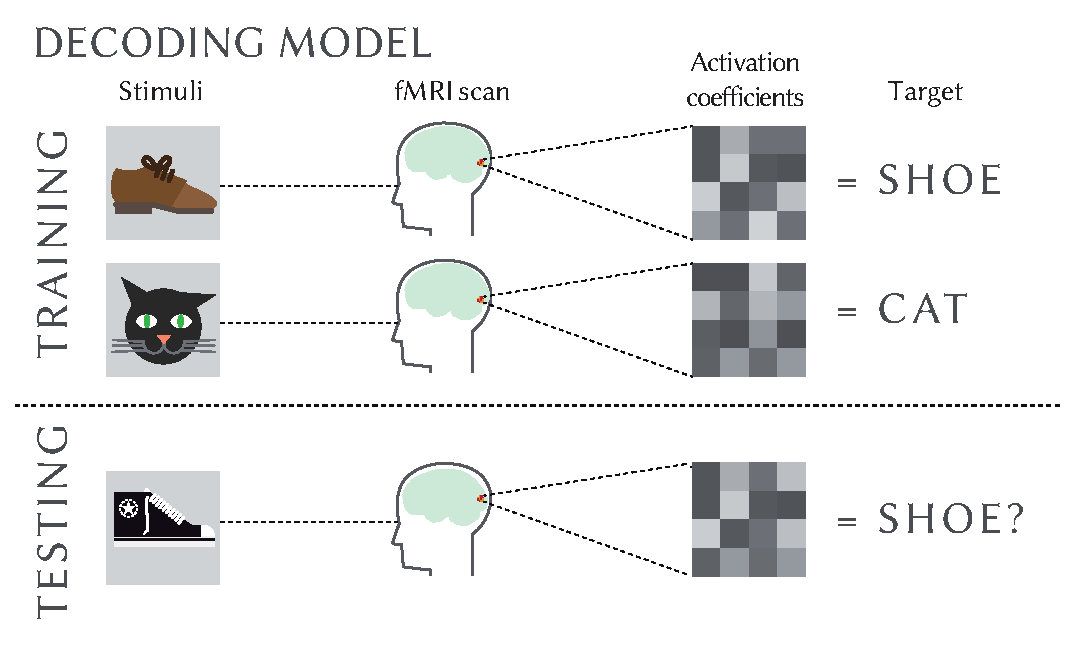
\includegraphics[width=1.05\linewidth]{chapter_2/decoding2.pdf}
\caption{Decoding models use patterns of activity to discriminate between cognitive states. Different \gls{activation coefficient}s reflect different mental states; for example, those associated with different images viewed by the subject. In a training phase, the classifier will learn to discriminate between activity patterns measured under different cognitive states. In the testing phase the generalization performance of the trained model is quantified by evaluating the classifier on the testing set and comparing the output of the classifier with the true labels associated with the stimuli. Adapted from~\citep{smith2013reading}.}\label{fig:c2_decoding}
\end{figure}

% This decoding approach can be used to provide answers to some neuroscientific questions. This question is a hypothesis testing problem that can be studied both on a single subject or a multi-subject study. In the first case the inference that we want to establish is whether the classifier designed on data from a given brain area of one subject is accurate enough to claim that the area actually encodes some information about the stimuli. 

The neuroscientific questions that brain decoding is able to address are commonly shaped within the statistical hypothesis testing framework. The inference that we want to establish is whether the classifier designed on data from a given brain area of one subject is accurate enough to claim that the area encodes some information about the stimuli. In this setting, the null hypothesis is that a given brain area does not contain stimuli-related information. The ability of the classifier to correctly predict some information about the stimulus is considered a positive evidence in support of the alternate hypothesis of presence of stimuli-related information within the brain activity.



% Although it is possible to perform decoding directly on raw BOLD
% signal~\citep{Mourao-Miranda2007, miyawaki2008visual}, the common approach consists in extracting the activation coefficients from
% the BOLD signal by using a known form of the Hemodynamic Response Function and the linear-time-invariant property of BOLD signal\label{chapter1_GLM} described in section \ref{chapter1_GLM} and use this estimates as input to the decoding model. 


% Compared to Statistical Parametric Maps, decoding models offer the advantage that the model relating activation coefficients to stimuli can consider several voxels at the same time ({\blue not making the same inference!!}). In the literature the decoding model is often described as a multi-variate approach while SPMs are univariate approaches. Multi-variate approaches have the advantage that they are able to discriminate conditions based on a distributed pattern of activity, contrary to univariate approaches that can only discriminate conditions based on a single activation coefficient. {\blue This translates in greater statistical power but also in a higher risk of overfitting due to the high dimensionality of the activation coefficients. In these settings the the number of voxels (dimensions) is typically higher than the number of activation coefficients (samples), thus the use of regularization and/or dimensionality reduction approaches is necessary}.



In~\citep{borghesani:hal-00986606}, we have used decoding models to establish in which regions of the brain it is possible to decode different aspects of words representing real-world objects. One of the tasks was to decode the size of items from the words representing those objects. In this case, the different stimuli are ordered according to their relative size, so the target variable is of ordinal nature. We predict the target variable from the brain activation on 6 anatomically defined regions of interest (ROI, which correspond to different Brodman areas). The metric is Kendall tau, which is a measure of the association between two measured quantities. This metric lies between -1 and 1. This metric and the used model will be presented in full detail in Chapter~\ref{chap:decoding_ordinal}).

% The Ridge regularization parameter chosen by nested cross-validation and the scores reported are the cross-validations scores using a leave-one-session out scheme.

\begin{figure*}
\mbox{
{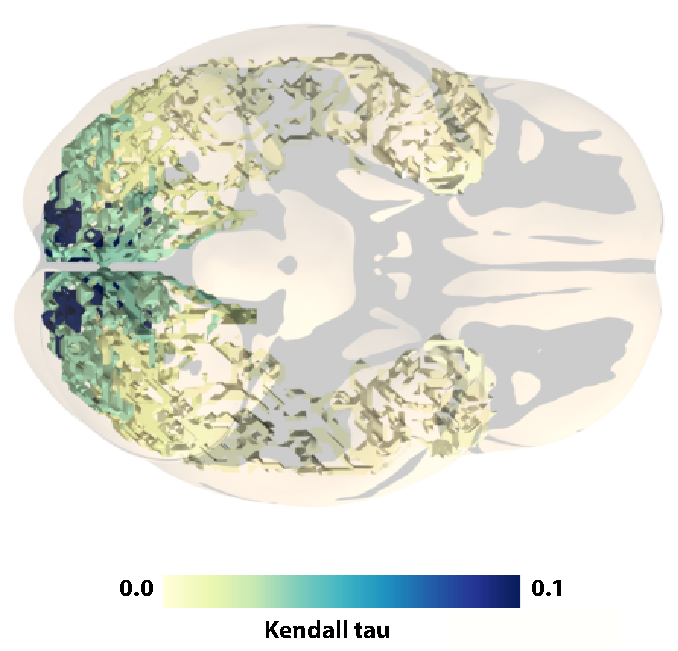
\includegraphics[width=0.40\linewidth]{chapter_2/word_length_horiz.pdf}}
{\hspace{1cm}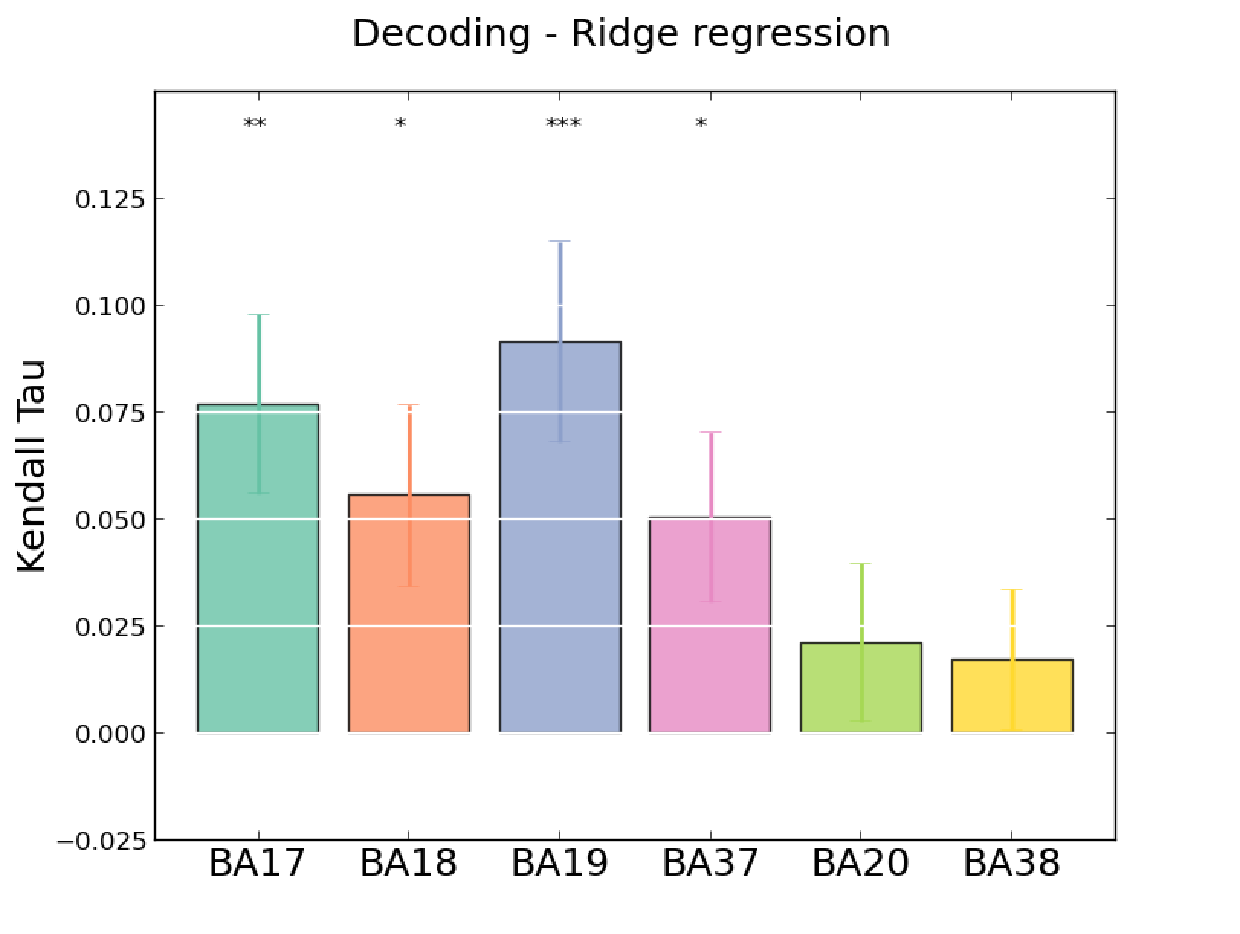
\includegraphics[width=0.55\linewidth]{chapter_2/vb_decode_size.png}}
}
\caption{Cross-validation scores for the prediction of the length of words from~\citep{borghesani:hal-00986606}. The metric is Kendall tau (higher is better). In the left, the same scores are depicted for the different regions (Brodman areas). 
}\label{fig:brain_score_length_vb}
\end{figure*}


As can be seen in Figure~\ref{fig:brain_score_length_vb}, this decoding model results in a higher decoding score in primary and secondary visual areas. In this case, a Wilcoxon signed-rank test was used to asses the statistical significance ($p$-value $< 0.05$) of the scores. This is denoted by the $*$ symbol that reflects the significance of a Wilcoxon test that the mean is significantly different than zero, $*$ = $p$-val $< 0.05$, $**$ = $p$-val $< 10^{-3}$, $***$ = $p$-val $< 10^{-6}$. This is achieved in Brodman areas BA17, BA18 and BA19. This experiments allows us to establish that the aforementioned areas encode some information related to the size of the stimuli.




% it is possible to decode the size of  objects from its conceptual representation (recall that stimuli are words and not images) in the aforementioned brain regions.

% {\blue Decoding vs statistical inference}. Although related, decoding and the application of classical inference to fMRI detailed before answer slightly different questions.  From a cognitive point of view, one of the main advantages of decoding models over classical inference {\blue is that they are able to use information from multiple voxels at the same time}.



\subsection{fMRI-based brain activity encoding}\label{chap2_encoding}

fMRI-based \emph{encoding} models (also known as \emph{voxel-wise modelling}) \citep{thirion2006, Kay2008, mitchell2008predicting}, seek to predict the patterns of brain activity from the the stimuli features. A machine learning model is learned from the stimuli features to the \gls{activation coefficient}s of a single voxel.
%\marginnote{Although it would be possible to construct encoding models that predict a set of voxels simultaneously, the models that have appeared in the literature until now consider the different voxels separately.} 
The sample space in this case is the space of features derived from the stimuli, e.g. spatial Dirac functions in~\citep{thirion2006} or Gabor filters in the case of natural images~\citep{Kay2008, Naselaris2014}. The predicted activation coefficient can then be compared to the true activation coefficient measured on left out data by using some distance metric such as Pearson or Spearman correlation coefficient.

% {\blue What inference can you make with encoding models ?}

\begin{figure}
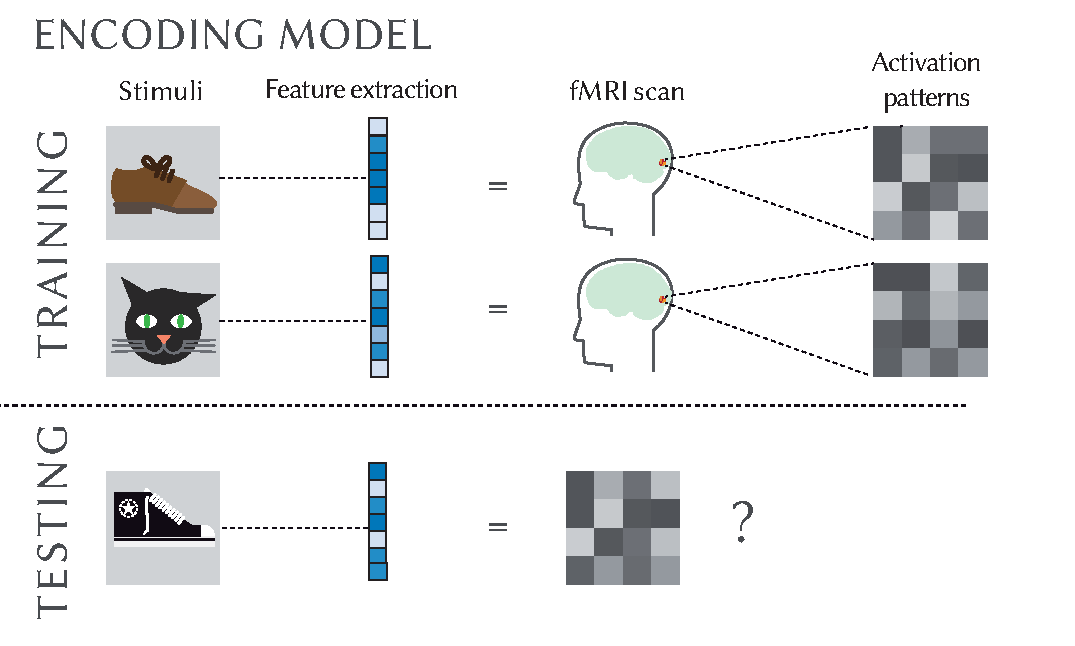
\includegraphics[width=1.\linewidth]{chapter_2/encoding.pdf}
\caption{ In an encoding model the patterns of brain activity are predicted by a machine learning model based on the stimuli features. The sample space in this case is the space of features derived from the stimuli, e.g. a set of Gabor filters in~\citep{Kay2008}. The predicted activation coefficient can then be compared to the true activation coefficient measured on left out data by using some distance metric such as Pearson's correlation coefficient. Adapted from~\citep{smith2013reading}.}\label{fig:c2_encoding}
\end{figure}

To the best of my knowledge, all of the encoding models that have been
published in the literature make assume a use of linear relationship features to the activation coefficients. That is, they assume that there is a  mapping from the stimulus space to the feature space that, and a linear mapping between the feature space and the activity space. However, the success of an encoding model depends in great measure on deriving the right features from the stimuli, a transformation that might be nonlinear. For example, \citet{naselaris2009bayesian} constructed two different models for each voxel: a model based on phase-invariant Gabor wavelets, and a semantic model that was based on a scene category label for each natural scene. The authors showed that the Gabor wavelet model provided good predictions of activity in early visual areas, while the semantic model predicted activity at higher stages of visual processing. 

Encoding and decoding can be seen as complementary operations: while encoding uses stimuli to predict activity,  decoding uses activity to predict information about the stimuli. Furthermore, encoding offers the advantage over decoding models that they can be used to predict information about an unseen stimuli. In this setting encoding models have been used to reconstruct stimuli from brain activity patterns in~\citep{miyawaki2008visual, naselaris2009bayesian, nishimoto2011reconstructing}. A similar setting was used in~\citep{Kay2008} to identify natural images. Here, the predicted activation coefficients were used to select the image that matched most closely the measured activation coefficients.



\section{Conclusion}

In this chapter we  have presented the statistical methods that will be used for drawing conclusions from fMRI experiments in further chapters. The chapter is divided into two sections. In the first section we have introduced the framework of statistical hypothesis testing and presented several parametric and non-parametric tests. We have presented an application of voxel-wise hypothesis testing known as Statistical Parametric Maps (SPMs).



In the second part of this chapter we have presented the setting of supervised learning. We described different surrogate loss functions and penalties that have found applications in the context of fMRI analysis. The surrogate loss functions that we described are  as Support Vector Machines, Logistic Regression, Support Vector Regression and Least Squares. The penalties that we have present are: squared $\ell_2$, $\ell_1$, elastic-net ($\ell_2^2 + \ell_1$) and total-variation (TV). Finally, we present two neuroscientific problems that can be model as a supervised learning problem: \emph{encoding} and \emph{decoding}.


\newpage


\begin{fullwidth}
\bibliographystyle{plainnat}
\bibliography{chapter_2/biblio2}
\end{fullwidth}


\begin{fullwidth}
\chapter{Data-driven HRF estimation for encoding and \\ \mbox{decoding} models}\label{chap:hrf_estimation}
\end{fullwidth}

\markright{{~{\rm \ref{chap:hrf_estimation}}. Data-driven HRF estimation}\hfill}{}

\newthought{We have seen} in Chapter~\ref{chap:stats_fmri} that encoding and decoding models take as input  brain activation coefficients (also known as activation patterns or beta-maps). These are usually computed by means of the general linear model (GLM), which
relies on a \mbox{data-independent} \emph{canonical} form of the hemodynamic response function
(HRF).


In this chapter we describe a novel method for the simultaneous estimation of HRF and activation coefficients based on low-rank modeling, forcing the estimated HRF to be equal across events or experimental conditions,
 yet permitting it to differ across voxels. The estimation of this model leads to
an optimization problem that we propose to solve with using a
\mbox{quasi-Newton} method, exploiting fast gradient computations. 
We compare 10 different HRF modeling methods in terms of encoding and decoding
score on two different datasets. These results show that the \mbox{R1-GLM} model
outperforms competing methods in both encoding and decoding
settings, positioning it as an attractive method both from the points of view
of accuracy and computational efficiency.

\hspace{20pt}
\begin{shaded}
The contributions developed in this chapter have been published in:
\begin{itemize}
\item F. Pedregosa, M. Eickenberg, P. Ciuciu, and B. Thirion, \emph{``Data-driven HRF estimation for encoding and decoding models''} NeuroImage, Volume 104, 1 January 2015, Pages 209-220.

\item F. Pedregosa, M. Eickenberg, B. Thirion, and A. Gramfort, \emph{“HRF estimation improves sensitivity of fMRI encoding and decoding models”} Proc. 3nd Int. Work. Pattern Recognit. NeuroImaging, 2013.
\end{itemize}
\end{shaded}

\newpage
\vspace*{\fill}
\minitoc
\vspace*{\fill}
\newpage


\section{Increased sensitivity via HRF estimation}

\begin{marginfigure}[4cm]
\hspace{-20pt}\includegraphics[width=1.2\linewidth]{chapter_3/hrfs_age.pdf}
\caption{
	The HRF can vary substantially between subjects, brain regions and age. In \citet{colonnese2007development}, the authors studied the evolution of the HRF across age in rats. By comparing fMRI measurements with electrophysiological recordings, they observed two significant trends as age increased: growing amplitude and decreasing time to peak. In the figure, estimated HRF for three groups of rats (with age P13-15 < P20-30< Adult). Source: \citep{colonnese2007development}. A comparison of the HRF in human subjects was performed in~\citep{badillo2014multi}.
}
\end{marginfigure}


fMRI acquisitions consist of successive brain scans, given in intervals ranging from 1 to 4 seconds. The extraction of time-independent \gls{activation coefficient} from the BOLD time course is commonly done with a model known as Linear General Model
(GLM)~\citep{Friston1995}. While
this approach has been successfully used in a wide range of studies, it does
suffer from limitations~\citep{Poline2012}. For instance, the GLM commonly
relies on a \mbox{data-independent} \emph{reference} form of the hemodynamic response function
(HRF) to estimate the activation coefficient (also known as \emph{canonical HRF}). However it is
known~\citep{Handwerker2004,Badillo2013} that the shape of this response function
can vary substantially across subjects, age and brain regions. This suggests that an adaptive modeling of this
 response function should improve the accuracy of subsequent analysis.

% \emph{feature-extraction} model that extracts 

% In this section we describe a method that allows to estimate time-independent \gls{activation coefficient} given the BOLD time course. {\blue Feature extraction}. This model is known as the \emph{general linear model}~\citep{Friston1995}. In this chapter we describe the main assumptions behind this model: a known form of the hemodynamic response function and the linear-time-invariant property between the BOLD signal and the neural response. 

% We have seen in Chapter 2 that both encoding and decoding models take as input voxel-wise activation coefficients. These are commonly are computed by means of the General Linear Model
% (GLM)~\citep{Friston1995}. While
% this approach has been successfully used in a wide range of studies, it does
% suffer from limitations~\citep{Poline2012}. For instance, the GLM commonly
% relies on a \mbox{data-independent} \emph{reference} form of the hemodynamic response function
% (HRF) to estimate the activation coefficient (also known as \emph{canonical HRF}). However it is
% known~\citep{Handwerker2004,Badillo2013} that the shape of this response function
% can vary substantially across subjects, age and brain regions. This suggests that an adaptive modeling of this
%  response function should improve the accuracy of subsequent analysis.

To overcome the aforementioned limitation, Finite Impulse Response (FIR) models have been
proposed within the GLM framework~\citep{Dale1999,Glover1999}.
These models do not assume any particular shape for the HRF and amount to
estimating a large number of parameters in order to identify it. 
While the FIR-based modeling makes it possible to estimate the
activation coefficient and the HRF simultaneously, the increased flexibility
has a cost. The estimator is less robust and prone to overfitting, i.e. to generalize poorly to unseen data. 
In general, FIR
models are most appropriate for studies focused on the characterization of the
shape of the hemodynamic response, and not for studies that are primarily
focused on detecting activation~\cite[Chapter~5]{Poldrack}.

Several strategies aiming at reducing the number of degrees of freedom of the
FIR model - and thus at limiting the risk of overfitting - have been proposed.
One possibility is to constrain the shape of the HRF to be a linear
combination of a small number of basis functions. A common choice of basis is 
formed by three elements consisting of a reference HRF as well as its time and dispersion
derivatives~\citep{friston1998nonlinear}, although it is also possible to compute a
basis set that spans a desired function
space~\citep{Woolrich2004}. More generally, one can also define a parametric
model of the HRF and estimate the parameters that best fit this
function~\citep{Lindquist2007}. However, in this case the estimated HRF may no longer be a linear function of the input parameters. 

Sensitivity to noise and overfitting can also be reduced through
regularization. For example, temporal regularization has been used in the
smooth FIR ~\citep{Goutte2000,Ciuciu2003,Casanova2008} to favor solutions with
small second order time derivative. These approaches require the setting of
one or several hyperparameters, at the voxel or potentially at the parcel
level (if several voxels in a pre-defined parcel are assumed to share some aspects of the HRF time course). Even if efficient techniques such as generalized   
\mbox{cross-validation}~\citep{golub1979generalized} can be used to choose the
regularization parameters, these methods are inherently more costly than 
\mbox{basis-constrained} methods. \mbox{Basis-constrained} methods also require
setting the number of basis elements; however, this parameter is not
continuous (as in the case of regularized methods), and in practice only few
values are explored: for example the 3-element basis set formed by a reference HRF
plus derivatives and the FIR model.  This paper focuses on basis-constrained
regularization of the HRF to avoid dealing with hyperparameter selection with
the goal of remaining computationally attractive.  A different approach to
increase robustness of the estimates consists in linking the estimated HRFs
across a predefined brain parcel, taking advantage of the spatially dependent nature of
fMRI~\citep{Wang2013}. However, \mbox{hemodynamically-informed}
parcellations~\citep{Chaari2012,Badillo2013a} rely on the computation of 
a large number of estimations at the voxel or \mbox{sub-parcel} level.
In this setting, the development of voxel-wise estimation procedures is complementary to the
development of parcellation methods in that more robust estimation
methods at the voxel level would naturally translate into more 
robust parcellation methods. In this thesis we focus on voxel-wise
estimation methods.


\paragraph{Contribution}

In this chapter we have described a method for the simultaneous estimation of HRF and activation coefficients based on low-rank modeling. While the assumptions of this model are not novel (cf.~\citep{Makni2008,vincent2010spatially,Degras2014}), the formulation of this model as a least squares problem with a rank-one constraint is a novel contribution. This formulation allows to efficiently solve the problem using gradient-based methods.
Finally, we evaluate the proposed model on three publicly available datasets. 

% {\blue With respect to the work published in ~\citep{Pedregosa2015209}, we have included in this chapter the results on a new datasets and examined the gain obtained by this model across different regions of the brain}.

\section{Methods}

In this section we describe different methods for extracting the HRF and
activation coefficients from BOLD signals. We will refer to each different
stimulus as {\it condition} and we will call {\it trial} a unique presentation
of a given stimulus. We will denote by $k$ the total number of stimuli, $\B{y} \in \RR^n$
the BOLD signal at a single voxel and $n$ the total number of images acquired.

\subsection{Basis-constrained GLM}



The reference HRF models a general response function that has been proven successful under a wide range of circumstances. However, a number of studies have shown that the shape of the hemodynamic response differ substantially among subjects~\citep{Aguirre1998360} and brain regions~\citep{Schacter1997259}. One popular approach to model small offsets in the time to peak and dispersion is to consider that the HRF is modeled from a basis set consisting of the reference HRF plus its derivative with respect to time and dispersion (see Figure~\ref{fig:hrf_basis}). The rationale for considering this basis set comes from the fact that it corresponds to the first-order approximation to the Taylor expansion of the reference HRF. Given the reference HRF, $h(t)$, a time-shifted version of the hemodynamic response can be described as $h(t + \delta)$. A Taylor series expansion of $h(t + \delta)$ with respect to $\delta$ gives the approximation $h(t) + \delta h'(t) + \ldots$~, implying that small offsets can be modeled by considering a linear combination of the reference HRF plus its time derivative. In similar fashion we can model small perturbations in dispersion (the width of the response) by considering the reference HRF plus its dispersion derivative. 


\begin{figure*}
\includegraphics[width=.5\linewidth]{figures/chapter_1/canonical_hrf_basis.pdf}
\includegraphics[width=.5\linewidth]{figures/chapter_1/canonical_hrf_generated.pdf}
\caption{A popular basis set to generate a family of HRF functions is the ``reference HRF plus derivatives''. In the left plot, we show a reference HRF together with its time and dispersion derivatives. This basis set can model small variations in temporal shifts and dispersion with respect to the reference HRF. In the right plot we show a sample set of HRFs generated by this basis. The weights of these response functions are Gaussian random vectors centered around the reference HRF.}\label{fig:hrf_basis} 
\end{figure*}

A popular example of basis set is presented in Figure~\ref{fig:hrf_basis} and consists of the reference HRF plus its time and dispersion (width) derivatives. While in the GLM with fixed HRF each regressor of the design matrix consisted of the convolution of the reference HRF with the stimulus function, in this case each regressor consist in the convolution of a basis element with the stimulus function. This results in a  design matrix of size $n \times d k$ instead of $n \times k$, where $d$ is the number of basis elements. If $d=1$ and the basis element is the reference HRF, then this setting coincides with the standard GLM. A least squares estimate of the activation coefficients $\hat{\bfbeta} = \argmin_{\bfbeta}\|\B{y} - \B{X}\bfbeta \|^2$ will result in a vector of $d$ elements for each condition. 


The design matrix of a GLM using the basis set of the ``refence HRF plus derivatives'' is shown in Figure~\ref{fig:glm1}. The columns in this design matrix are each one of the basis elements convolved with the stimulus function for the different conditions.




\subsection{Basis and rank-constrained GLM}

In the basis-constrained GLM, the HRF estimation is performed 
independently for each condition. This method works reliably whenever
the number of conditions is small, but in experimental designs with a large
number of conditions it performs poorly due to the increased variance of the estimates.
% put ref?

% In this model we promote a common HRF
% across the various stimuli, which should result in more robust estimates~\citep{Makni2008,vincent2010spatially}.
In this work we consider a model in which a common HRF is shared
across the different stimuli. Besides the estimation of the HRF,
a unique coefficient is obtained per column of our event
matrix. This amounts to the estimation of $k + d$ free parameters
instead of $k \times d$ as in the standard basis-constrained GLM setting.

The novelty of our method stems from the observation that the formulation of the GLM with a
common HRF across conditions translates to a rank constraint on the vector of estimates. 
This assumption amounts to enforcing the vector of
estimates to be of the form $\bfbeta_{\B{B}} = [\mathbf{h} {\beta}_1, \mathbf{h} \beta_2, \cdots, \mathbf{h}
\beta_k]$ for some HRF $\mathbf{h} \in \RR^d$ and a vector of coefficients $\bfbeta \in \RR^k$. More compactly, this can be written as $\bfbeta_{\B{B}} = \vecop(\B{h}
\bfbeta^T)$. This can be
seen as a constraint on the vector of coefficients to be the vectorization of a rank-one
matrix, hence the name {\it Rank-1 GLM (R1-GLM)}.


\begin{figure*}[t]
\centering \includegraphics[width=0.8\linewidth]{figures/chapter_1/glm_3hrf.pdf}
\caption{A basis-constrained GLM design matrix. The basis set consists of the reference HRF plus its time and dispersion derivative. As in the GLM introduced in Chapter~\ref{chap:intro_fmri} (Fig.~\ref{fig:glm1}), each column is the convolution of one basis function with the stimulus function. Here, the usage of 3 basis functions (instead of one) results in a design matrix with $3 k$ regressors}\label{fig:glm_3hrf}
\end{figure*}


In this model, the coefficients have no longer a closed form expression,
but can be estimated by minimizing the following loss function. Given $\B{X}_{\B{B}}$ and $\B{y}$ as before, $\B{Z} \in \RR^{n \times q}$ a matrix of nuisance parameters such as drift regressors, we define $F_{\text{R1}}(\B{h}, \bfbeta, \bfomega, \B{X}_{\B{B}}, \B{y}, \B{Z}) = \frac{1}{2}\|\mathbf{y} - \mathbf{X}_{\B{B}} \vecop(\B{h} \bfbeta^T) - \B{Z} {\bfomega}\| ^2$ to be the objective function to be minimized. The optimization problem reads:
%
\begin{eqnarray}
\label{eq:r1}
\begin{aligned}
\hat{\B{h}}, ~\hat{\bfbeta},~ \hat{\bfomega} ~=~& \argmin_{\B{h}, \bfbeta, {\bfomega}} ~ F_{\text{R1}}(\B{h}, \bfbeta, \bfomega, \B{X}_{\B{B}}, \B{y}, \B{Z})\\
&\text{subject to } \|\B{B} \B{h}\|_{\infty} = 1 \text{ and } \langle \B{B} \B{h}, \B{h}_{\text{ref}}\rangle > 0 \enspace ,
\end{aligned}
\end{eqnarray}
%
The norm constraint is added to avoid the scale ambiguity between $\B{h}$ and $\bfbeta$
and the sign is chosen so that the estimated HRF correlates
positively with a given reference HRF $\B{h}_{\text{ref}}$.
Otherwise the signs of the HRF and $\bfbeta$ can be simultaneously flipped without changing
the value of the cost function. Within its feasible set, the optimization problem
is {\it smooth} and is convex with respect to $\B{h}$, $\bfbeta$ and $\bfomega$,
 however it is not {\it jointly convex} in variables $\B{h}$, $\bfbeta$ and $\bfomega$.

From a practical point of view this formulation has a number of advantages.
First, in contrast with the GLM without rank-1 constraint the estimated
coefficients are already factored into the estimated HRF and the activation
coefficients. That is, once the estimation of the model parameters
from Eq.~\eqref{eq:r1} is obtained, $\hat{\bfbeta}$ is a vector of size $k$ and $\hat{\B{h}}$ is a
vector of size $d$ that can be both used in subsequent analysis, while in models
without rank-1 constraint only the vector of coefficients (equivalent to 
$\text{vec}(\B{h} \bfbeta^T)$ in rank-1 constrained models) of size $k
\times d$ is estimated. In the latter case, the estimated HRF and the beta-maps
still have to be extracted from this vector by methods such as normalization by the peak of the HRF,
averaging or projecting to the set of Rank-1 matrices.

Second, it is readily adapted to prediction on unseen trials. While for
classical (non rank-1 models) the HRF estimation is performed per condition with no HRF associated with unseen conditions, in this setting, because the
estimated HRF is linked and equal across conditions it is natural to use this
estimate on unseen conditions. This setting occurs often in encoding models 
where prediction on unseen trials is part of the cross-validation procedure.

This model can also be extended to a parametric HRF model. That is,
given the hemodynamic response defined as a function $h: \RR^{d_1} \to \RR^d$ of some parameters
$\bfalpha$, we can formulate the analogous model of Eq.~\eqref{eq:r1} as an
optimization over the parameters $\bfalpha$ and $\bfbeta$ with the design matrix
$\B{X}_{\text{FIR}}$ given by the convolution of the event matrix with the FIR basis:
%
\begin{eqnarray}
\label{eq:r1_parametric}
\begin{aligned}
\hat{\bfalpha}, ~\hat{\bfbeta}, ~\hat{\bfomega} ~=~&\argmin_{\bfalpha, \bfbeta, \bfomega} 
F_{\text{R1}}(h(\bfalpha), \bfbeta, \bfomega, \B{X}_{\text{FIR}}, \B{y}, \B{Z}) \\
&\text{subject to } \| h(\bfalpha)\|_{\infty} = 1  \text{ and } \langle h(\bfalpha), \B{h}_{\text{ref}} \rangle > 0
\end{aligned}
\end{eqnarray}

In section \ref{sub:optim} we will discuss optimization strategies for both
models.

% \subsection{Alternative formulations}

% We present two alternative formulations

\subsection{Extension to separate designs}

\begin{marginfigure}[8cm]
\center \includegraphics[width=.6\linewidth]{chapter_3/ls-s.pdf}
\caption{In the GLM with separate designs model of~\citet{Mumford2012}, the design matrix contains two regressors. The first one is the
regressor associated with a given condition and the second one is the sum of all
other regressors. Source: \citep{Turner2012}}
\end{marginfigure}

An extension to the classical GLM that improves the estimation with correlated
designs was proposed in~\citep{Mumford2012}.
In this setting, each voxel is modeled as a linear combination of two
regressors in a design matrix $\B{X}_\text{GLM}$. The first one is the
regressor associated with a given condition and the second one is the sum of all
other regressors. This results in $k$ design matrices, one for each condition.
The estimate for a given condition is given by the first element in the two-dimensional
array ${\B{X}_{\text{S}i}}^{\dagger} \B{y}$, 
where $\B{X}_{\text{S}i}$ is the design matrix for
condition $i$. We will 
denote this model GLM with separate designs (GLMS). It has been reported to find
a better estimate in rapid event designs leading to a boost in accuracy for
decoding tasks~\citep{Mumford2012, Schoenmakers2013, Lei2013}.

This approach was further extended in~\citep{Turner2012} to
include FIR basis instead of the predefined canonical function. Here we employ it 
in the more general setting of a  
predefined basis set. Given a set of basis
functions we construct the design matrix for condition $i$ as the columnwise
concatenation of two matrices $\B{X}^0_{\text{BS}i}$ and $\B{X}^1_{\text{BS}i}$.
$\B{X}^0_{\text{BS}i}$ is given by the columns associated
with the current condition in the GLM matrix and $\B{X}^1_{\text{BS}i}$ is
the sum of all other columns.
In this case, the vector of estimates is given by the first $d$ vectors of
$\B{X}_{\text{BS}i}^{\dagger} \B{y}$. See~\citep{Turner2012} for a more complete description of the matrices $\B{X}^0_{\text{BS}i}$ and $\B{X}^1_{\text{BS}i}$.

It is possible to use the same rank-1
constraint as before in the setting of separate designs, linking the HRF 
across conditions. We will refer to this model as \emph{Rank-1 GLM with separate designs (R1-GLMS)}. In this case the objective function has the form
$F_{\text{R1-S}}(\B{h}, \bfbeta, \bfomega, \B{r}, \B{X}_{\B{B}}, \B{y}, \B{Z}) = \frac{1}{2}\sum_i^k \|\B{y} - \beta_i \B{X}^0_{\text{BS}i} \B{h} - r_i \B{X}^1_{\text{BS}i} \B{h} - \B{Z} \bfomega\| ^2 $, where $\B{r} \in \RR^d$ is a vector representing the activation of all events except the event of interest and 
will not be used in subsequent analyses. We can 
compute the vector of estimates $\hat{{\bfbeta}}$ as the solution to the optimization
problem
%
\begin{eqnarray}
\label{eq:r1_separate}
\begin{aligned}
\hat{\bfbeta}, ~\hat{\bfomega},~\hat{\B{h}},~\hat{\bf{r}} ~= ~&\argmin_{\B{h}, \bfbeta, \bfomega, \B{r}} F_{\text{R1-S}}(\B{h}, \bfbeta, \bfomega, \B{r}, \B{X}_{\B{B}}, \B{y}, \B{Z}) \\
&\text{subject to } \|\B{B} \B{h}\|_{\infty} = 1 \text{ and } \langle \B{B} \B{h}, \B{h}_{\text{ref}} \rangle > 0
\end{aligned}
\end{eqnarray}
%


\subsection{Optimization}
\label{sub:optim}


For the estimation of rank-1 models on a full brain volume, a  model is estimated at each voxel separately. Since a typical brain volume contains more than 40,000 voxels, the efficiency of the estimation at a single voxel is of great importance. In this section we will detail an efficient procedure based on quasi-Newton methods for the estimation of R1-GLM and R1-GLMS models on a given voxel.


One approach to minimize \eqref{eq:r1} is to alternate the minimization
with respect to the variables $\bfbeta$, $\B{h}$ and $\bfomega$. By recalling the Kronecker product identities~\cite[Chapter 4.3]{horn1991topics}, and using the identity \(\vecop(\B{h}\bfbeta^T) = \bfbeta\otimes \B{h}\)
we can rewrite the objective function~\eqref{eq:r1} to be minimized as:
%
\begin{gather}
\label{eq:kron}
\frac{1}{2}\|\B{y} - \B{X}_{\B{B}} (\bfbeta \otimes \B{h}) - \B{Z} \bfomega\| ^2 = \\ \frac{1}{2}\|\B{y} - \B{X}_{\B{B}} (\B{I} \otimes \B{h}) \bfbeta - \B{Z} \bfomega\| ^2 = \\ \frac{1}{2}\|\B{y} - \B{X}_{\B{B}} (\bfbeta \otimes \B{I}) \B{h} - \B{Z} \bfomega\|^2 \enspace.
\end{gather}
%
Updating $\B{h}$, $\bfbeta$ or $\bfomega$ sequentially thus amounts to solving a (constrained) least squares
problem at each iteration. A similar procedure is detailed in~\citep{Degras2014}. However, this approach requires computing the
matrices $\B{X}_{\B{B}} (\bfbeta \otimes \B{I})$ and $\B{X}_{\B{B}} (\B{I} \otimes \B{h})$ at each iteration, which are typically dense,
resulting in a high computational cost per iteration. Note also that the optimization problem is not jointly convex in variables $\B{h}, \bfbeta, \bfomega$, therefore we cannot apply convergence guarantees from convex analysis.

We rather propose a more efficient approach by optimizing both variables jointly. We define a 
global variable $\B{z}$ as the concatenation of $(\B{h}, \bfbeta, \bfomega)$ into a single vector, $\B{z} = \vecop([\B{h}, \bfbeta, \bfomega])$,
 and cast the problem as an optimization with respect to this new variable.
Generic solvers for numerical
optimization~\citep{nocedal2006numerical} can then be used. The solvers that we will consider take as
input an objective function and its gradient. In this case, the partial derivatives with respect to variable $\B{z}$ can be written as 
$\partial F_{\text{R1}} / \partial \B{z} = \vecop([\partial F_{\text{R1}} / \partial \B{h}, \partial F_{\text{R1}} / \partial{\bfbeta}, \partial F_{\text{R1}} / \partial {\bfomega}])$, whose expression can be
easily derived using the aforementioned Kronecker product identities:
%
\begin{equation*}
    \left\{
    \begin{aligned}
        \frac{\partial F_{\text{R1}}}{\partial \B{h}}=& - (\bfbeta^T \otimes \B{I}) \B{X}^T (\B{y} - \B{X} \vecop(\B{h} \bfbeta^T) - \B{Z} \bfomega) \\
        \frac{\partial F_{\text{R1}}}{\partial \bfbeta}=& - (\B{I} \otimes \B{h}^T) \B{X}^T (\B{y} - \B{X} \vecop(\B{h} \bfbeta^T) - \B{Z} \bfomega) \\
        \frac{\partial F_{\text{R1}}}{\partial \bfomega}=& - \B{Z}^T (\B{y} - \B{X} \vecop(\B{h} \bfbeta^T) - \B{Z} \bfomega)
    \end{aligned}
    \right.
\end{equation*}



If instead a parametric model of the HRF is used as in Eq.~\eqref{eq:r1_parametric}, the equivalent partial derivatives can be easily computed by the chain rule.


For the sake of efficiency, it is essential to avoid evaluating the Kronecker products naively,
 but rather reformulate them using the above mentioned Kronecker identities. For example, the matrix $\B{M} = \B{X} (\B{I} \otimes \B{h})$ should not be computed explicitly but should rather be stored as a linear operator such that when applied to a vector $\B{a} \in \RR^k$ it computes $M(\B{a}) = \B{X} (\B{a} \otimes \B{h})$, avoiding thus the explicit computation of $\B{I} \otimes \bfbeta$. 


Similar equations can be derived for the rank-1 model with separate designs of Eq.~\eqref{eq:r1_separate} (\mbox{R1-GLMS}), in which
case the variable $\B{z}$ is defined as the concatenation of $(\B{h}, \bfbeta, \bfomega, \B{r})$, i.e. $\B{z} = \vecop([\B{h}, \bfbeta, \bfomega, \B{r}])$. The gradient of $F_{\text{R1-S}}$ with respect to $\B{z}$ can be computed as $\partial F_{\text{R1-S}} / \partial \B{z}$ = $\vecop([\partial F_{\text{R1-S}} / \partial \B{h},$ $\partial F_{\text{R1-S}} / \partial{\bfbeta}, \partial F_{\text{R1-S}} / \partial {\bfomega}, F_{\text{R1-S}} / \partial {\B{r}}])$. The partial derivatives read:
%
\begin{equation*}
    \left\{
    \begin{array}{lcl}
        \frac{\partial F}{\partial \B{h}} &=& \sum_i^k - (\B{X}^0_{\text{BS}_i}\bfbeta_i - \B{X}^1_{\text{BS}_i} r_i)^T (\B{y} - \bfbeta_i \B{X}^0_{\text{BS}_i} h - w_i \B{X}^1_{\text{BS}_i} \B{h}) \\
        \frac{\partial F}{\partial \beta_i} &=& -(\B{X}^0_{\text{BS}_i} \B{h})^T (\B{y} - \bfbeta_i \B{X}^0_{\text{BS}_i} \B{h} - w_i \B{X}^1_{\text{BS}_i} \B{h}) \\
        \frac{\partial F}{\partial \omega_i} &=& -\B{Z}^T (\B{y} - \bfbeta_i \B{X}^0_{\text{BS}_i} \B{h} - w_i \B{X}^1_{\text{BS}_i} \B{h}) \\
        \frac{\partial F}{\partial r_i} &=& -(\B{X}^1_{\text{BS}_i} \B{h})^T (\B{y} - \bfbeta_i \B{X}^0_{\text{BS}_i} \B{h} - w_i \B{X}^1_{\text{BS}_i} \B{h}) \\
    \end{array}
    \right.
\end{equation*}

\begin{marginfigure}
\hspace{-10pt}\includegraphics[width=1.1\linewidth]{chapter_3/bench_r1.pdf}
\caption{Convergence of different first-order and quasi-newton optimization algorithms for the R1-GLM model on a single voxel. ``TNC'' and ``Newton-CG'' are two different implementations of the truncated Newton~\citep{nash1984newton} method (the first one in C and the second one in Python), ``L-BFGS-B'' is the Limited-memory BFGS algorithm with box constraints as implemented in~\citep{zhu1997algorithm}, ``trust-ncg'' is the Newton conjugate gradient trust-region 
algorithm and ``CG'' is the conjugate gradient algorithm, both of them described in~\citep{nocedal2006numerical}. We found that in general the L-BFGS-B gives the best performance among these methods.}
\end{marginfigure}

% \todo[color=blue!60, inline]{Used an eqnarray*, because this was awfully "align*"ed. It still isn't perfect though. Maybe we need to bind the left hand sides to the left? The same theoretically goes for the equations just above}

A good initialization plays a crucial role in the convergence of any iterative
algorithm. We have used as initialization for the R1-GLM and R1-GLMS models the solution given by the GLM with
separate designs (GLMS). Since the GLM with separate designs scales linearly in the number of voxels, this significantly reduces computation time whenever
an important number of voxels is considered.

Whenever the design matrix $\B{X}_{\B{B}}$ has more rows than columns (as is
the case in both datasets we consider with $\B{B}$ the 3HRF basis), it is possible to
find an orthogonal transformation that significantly speeds up the computation
of the Rank-1 model. Let $\B{Q}, \B{R}$ be the ``thin'' QR decomposition of
$\B{X}_{\B{B}} \in \RR^{n \times d k}$, that is, $\B{Q} \B{R} = \B{X}_{\B{B}}$ with $\B{Q}
\in \RR^{n \times d k}$ an orthogonal matrix and $\B{R} \in \RR^{d k \times d k}$ 
a triangular matrix. Because of the invariance of the Euclidean norm to orthogonal
transformations, the change of variable $\B{X}_{\B{B}} \leftarrow \B{Q}^T
\B{X}_{\B{B}}$, $\B{y} \leftarrow \B{Q}^T \B{y}$ yields a Rank-1 model in Eq.~\eqref{eq:r1}
with equivalent solutions. This reduces the size of the design matrix to a square triangular matrix of size $d k \times d k$ (instead of $n \times d k$) and reduces the explained variable $\B{y}$ to a vector of size $k d$ (instead of $n$). After this change of variable, the convergence of the Rank-1 model is significantly faster due to the faster computation of the objective function and its partial derivatives.  We have observed that the total running time of the algorithm can be
reduced by 30\% using this transformation.


Some numerical solvers such as L-BFGS-B~\citep{liu1989limited}
require the constraints to be given as box constraints. While our original
problem includes an equality constraint we can easily
adapt it to use convex box constraints instead.
We replace the equality constraint $\|\B{B h}\|_{\infty} = 1$ by
the convex inequality constraint $\|\B{B h}\|_{\infty} \leq 1$, which is equivalent
to the box constraint $-1 \leq (\B{B h})_i \leq 1$ supported by the above solver. 
However, this change of constraint
allows solutions in which $\B{h}$ can be arbitrarily close to zero. To avoid such
degenerate cases we add the smooth term $-\|\B{B}(:, 1) h_1\|^2 _2$ to the cost function. Since
there is a free scale parameter between $\B{h}$
and $\bfbeta$, this does not bias the problem, but forces $\B{B h}$ to lie as far as possible from the origin (thus saturating the box constraints). Once a descent
direction has been found by the \mbox{L-BFGS-B} method we perform a line search
procedure to determine the step length. The line-search
procedure was implemented to satisfy the strong Wolfe conditions~\citep{nocedal2006numerical}.
Finally, when the optimization algorithm has converged to a stationary point, 
we rescale the solution setting to ensure that the equality constraint. This still leaves a sign ambiguity between the estimated HRF and the associated beta-maps. To make these parameters identifiable, the sign of the estimated HRF will be chosen so that these correlate positively with the reference HRF.

We have compared several first-order (Conjugate Gradient), \mbox{quasi-Newton}
(L-BFGS) and Newton methods on this problems and found that in general \mbox{quasi-Newton} methods performed best in terms of computation time. In our
implementation, we adopt the L-BFGS-B as the default solver. 

In Algorithm~\ref{alg1} we describe an algorithm based on L-BFGS that can be used to optimize R1-GLM and R1-GLMS models (a reference implementation for the Python language is described in subsection Software). Variable $\B{r}$ is only used for the R1-GLMS method and its use is denoted within parenthesis, i.e. $(, \B{r})$, so that for the R1-GLM it can simply be ignored.
%
\begin{algorithm}
\caption{Optimization of R1-GLM and R1-GLMS models}
\label{alg1}
\begin{algorithmic}[1]
\REQUIRE Given initial points $\bfbeta_0 \in \RR^k, \B{h}_0 \in \RR^d, {\bfomega}_0 \in \RR^q ~(, \mathbf{r}_0 \in \RR^k)$, convergence tolerance $\epsilon > 0$, inverse Hessian approximation $\B{H}_0$. 
\ENSURE $\bfbeta_m, \B{h}_m$
\STATE {(Optional)}: Compute the QR decomposition of $\B{X}_{\B{B}}$, $\B{Q} \B{R} = \B{X}_{\B{B}}$, and replace $\B{X}_{\B{B}} \leftarrow \B{Q}^T \B{X}_{\B{B}}, \B{y} \leftarrow \B{Q}^T \B{y}$
\STATE Initialization. Set $m \leftarrow 0$, $\B{z} \leftarrow \vecop([\B{h}_0, \bfbeta_0, \bfomega_0 (, \B{r}_0)])$
\WHILE{$\|\nabla f\| > \epsilon$}
\STATE Compute search direction.  Set $\B{p}_m \leftarrow - \B{H}_m \nabla f(\B{h}_m, \bfbeta_m, \bfomega_m (, \B{r}_m))$
by means of the L-BFGS algorithm.
\STATE {Set $\B{z}_{m+1} = \B{z}_m + \gamma_m \B{p}_m$, where $\gamma_m$ is computed from a line search procedure subject to the box constraints $\|\B{h}_m\|_{\infty} \leq 1$}.
\STATE $m \leftarrow m+1$
\ENDWHILE 
\STATE Extract R1-GLM(S) parameters from $\B{z}_m$. Set $\B{h}_m \leftarrow \B{z}_m(1:d), \bfbeta_m \leftarrow \B{z}_m(d+1:m+d)$
\STATE Normalize and set sign so that the estimated HRF is positively correlated with a reference HRF: $q_m \leftarrow \|\B{h}_m\|_{\infty} \text{sign}(\B{h}_m^T \B{h}_{\text{ref}}),~ \B{h}_m \leftarrow \B{h}_m / q_m, ~\bfbeta_m \leftarrow \bfbeta_m q_m$
\end{algorithmic} 
\end{algorithm}

The full estimation of the R1-GLM with 3HRF basis for one subject of the
dataset described in section {\it Dataset 2: decoding of potential gain
levels} ($16 \times 3$ conditions, $720$ time points, $41,622$ voxels) took 14
minutes in a 8-cores Intel Xeon 2.67GHz machine. The total running time for
the 17 subjects was less than four hours.


\subsection{Software}

We provide a software implementation of all the models discussed in this section
in the freely available (BSD licensed) pure-Python package \textsf{hrf\_estimation}
available at {\href{https://pypi.python.org/pypi/hrf\_estimation}{https://pypi.python.org/pypi/hrf\_estimation}}~. This software is further described in Section~\ref{subsec:hrf_estimation}.

\section{Data description}

With the aim of making the results easily reproducible, we have
chosen two freely available datasets to validate our approach and to compare
different HRF modeling techniques.


\subsection{Dataset 1: encoding of visual information}\label{subsec:encoding_dataset}

The first dataset we will consider is 
described in~\citep{Kay2008,naselaris2009bayesian,kay2011data}. It contains 
BOLD fMRI responses in human subjects viewing natural images.
As in~\citep{Kay2008}, we performed
prediction of BOLD signal following the visual presentation of natural images
and compared it against the measured fMRI BOLD signal.
As the procedure consists of predicting the fMRI data
from stimuli descriptors, it is an {\it encoding} model.
This dataset is publicly available from \url{http://crcns.org}

Two subjects viewed 1750 training images, each presented twice,
and 120 validation images, each presented 10 times, while fixating a
central cross. Images were flashed 3 times per second (200 ms
on-off-on-off-on) for one second every 4 seconds, leading to a rapid
event-related design. The data were acquired in 5 scanner sessions on 5 different days,
each comprising 5 runs of 70 training images --each image  being presented twice
within the run-- and 2 runs of validation images showing 12 images,
10 times each. The images were recorded from the occipital cortex at a spatial resolution of 2mm$\times$2mm$\times$2.5mm
and a temporal resolution of 1 second. Every brain volume for each subject has been aligned to the first volume of the first run of the 
first session for that subject. Across-session alignment was performed manually. Additionally, 
data were temporally interpolated to account for slice-timing differences. See~\citep{Kay2008} for further preprocessing details. 



We performed local detrending using a Savitzky-Golay
filter~\citep{savitzky1964smoothing} with a polynomial of degree 4 and a window
length of 91 TR. The activation coefficients (beta-map) and HRF were extracted from
the training set by means of the different methods we would like to compare. The
training set consisted of 80\% of the original session (4 out of 5 runs). This
resulted in estimated coefficients (beta-map) for each of the $70 \times 4$
images in the training set.



We proceed to train the encoding model. The stimuli are handled as local image contrasts,  that are represented by spatially
smoothed Gabor pyramid transform modulus with 2 orientations and 4 scales. 
Ridge regression (regularization parameter chosen by Generalized Cross-Validation~\citep{golub1979generalized}) was then used to learn a
predictor of voxel activity on the training set. By using this encoding model
and the estimated HRF it is possible to predict the BOLD signal for the 70
images in the test set (20 \% of the original session). We emphasize that learning the HRF on the training set instead of on the full
dataset is necessary to avoid overfitting while assessing the quality of the estimated HRF by any
HRF-learning method: otherwise, the estimation of the HRF may incorporate specificities of the test set leading to artificially higher scores.

\begin{figure*}
\center\includegraphics[width=\linewidth]{chapter_3/nature_kay.pdf}
\caption{
\label{fig:kay_encoding}
	The original analysis performed in~\citep{Kay2008} allowed to identify natural images from human brain activity. The analysis consisted of two stages. In the first stage, model estimation, fMRI data were recorded while each subject viewed a large collection of natural images. These data were used to estimate an encoding model for each voxel. In the second stage, image identification, fMRI data were recorded while each subject viewed a collection of novel natural images. For each measurement of brain activity, they attempted to identify which specific image had been seen. This was accomplished by using the estimated encoding models to predict brain activity for a set of potential images and then selecting the image whose predicted activity correlates best with the measured activity. Source: Adapted from~\citep{Kay2008}.
}
\end{figure*}


In a first step, we perform the image identification task from~\citep{Kay2008} (Fig.~\ref{fig:kay_encoding}). From the training set we estimate the activation coefficients that will be used to compute the activation maps. We use an encoding model using Gabor filters that predicts the activation coefficient from the training stimuli. From the stimuli in the validation set we predict the activation coefficients that we then use to identify the correct image. The predicted image is the one yielding the highest correlation with the measured activity. This procedure mimics the one presented in~\citep[Supplementary material]{Kay2008}.



In a second step, we report score as the Pearson correlation between the measurements and the  predicted BOLD signal on left out data. The prediction of BOLD signal on the test set is performed from conditions that
were not present in the train set. In order to do this, an HRF for these conditions is necessary. As highlighted in the methods section, the
construction of an HRF for these conditions is ambiguous for non Rank-1
methods that perform HRF estimation on the different stimuli. In these cases
we chose to use the mean HRF across conditions as the HRF for unseen
conditions. Finally, linear predictions on the left out fold were compared to
the measured BOLD signals.

\subsection{Dataset 2: decoding of potential gain levels}

The second dataset described in~\citep{Tom2007} is a gambling task where each
of the 17 subjects was asked to accept or reject gambles that offered a 50/50
chance of gaining or losing money. The magnitude of the potential gain and
loss was independently varied across 16 levels between trials. Each gamble has
an amount of potential gains and potential losses that can be used as class label. In
this experiment, we only considered gain levels. This leads to the challenge of
predicting or \emph{decoding} the gain level from brain images. The dataset
is publicly available from \mbox{\url{http://openfmri.org}} under the name 
\emph {mixed-gambles task} dataset.

The data preprocessing included slice timing, motion correction, coregistration to the
anatomical images, tissue segmentation, normalization to MNI space and was
performed using the SPM 8 software through the
Pypreprocess\footnote{\url{https://github.com/neurospin/pypreprocess}}
interface.

For all subjects three runs were recorded, each consisting of 240 images with
a repetition time (TR) of 2 seconds and a stimulus presentation at every 4
seconds. In order to perform HRF estimation on more data than what is
available on a single run, we performed the estimation on the three runs
simultaneously. This assumes HRF consistency across runs, which was obtained by
concatenating the data from the three runs and creating a block-diagonal design matrix correspondingly (each block is the design of one run).


After training a regression model on 90\% of the data, we predict the gain level on the
remaining 10\%. As a performance measure we use Kendall tau rank correlation
coefficient~\citep{kendall1938new} between the true gain levels and the
predicted levels, which is a measure for the orderings of the data.  We argue
that this evaluation metric is better suited than a regression loss for this
task because of the discrete and ordered nature of the labels. Also, this loss
is less sensible to shrinkage of the prediction that might occur when penalizing a
regression model~\citep{bekhti:hal-01032909}. The Kendall tau coefficient always lies within the interval
$[-1, 1]$, with $1$ being perfect agreement between the two rankings and $-1$
perfect disagreement. Chance level lies at zero. This metric is equivalent to minimizing the number of the pairwise inversions, which was was previously
proposed for fMRI decoding with ordered labels in~\citep{pedregosa:hal-00717990}.


\section{Results}

In order to compare the different methods discussed previously, we ran
the same encoding and decoding studies while varying the
estimation method for the activation coefficients (beta-maps). The
methods we considered are standard GLM (denoted \gls{GLM}), GLM with separate
designs (GLMS), Rank-1 GLM (R1-GLM) and Rank-1 GLM with separate designs
(R1-GLMS). For all these models we consider different basis sets for
estimating the HRF: a set of three elements formed by the reference HRF and
its time and dispersion derivative, a FIR basis set (of size 20 in the
first dataset and of size 10 in the second dataset) formed by the canonical vectors
and the single basis set formed by the reference HRF (denoted ``fixed HRF''), which
in this case is the HRF used by the SPM 8 software.

It should be reminded that the focus of this study is not the study of the HRF
in itself (such as variability across subjects, tasks or regions) but instead
its possible impact on the accuracy of encoding and decoding paradigms. For
this reason we report encoding and decoding scores but we do not investigate
any of the possible HRF variability factors.

\subsection{Dataset 1: encoding of visual information}

In the original study, 500 voxels were used to perform image identification. These voxels were selected as the voxels with the highest correlation with the true BOLD signal on left-out data using a (classical) GLM with the reference HRF. These voxels are therefore not the ones naturally benefiting the most from HRF estimation. 


We first present the scores obtained in the image identification task for different variants of the GLM. This can be seen in Figure~\ref{fig:identification_scores}. The displayed score is the count of correctly identified images over the total number of images (chance level is therefore at 1/120). The identification algorithm here only uses the beta-maps obtained from the train and validation set. This makes the estimation of the HRF an intermediate result in this model. However, we expect that a correct estimation of the HRF directly translates into a better estimation of the activation coefficients in the sense of being able to acheive higher predictive accuracy. Our results are consistent with this hypothesis and in this task the rank-one (R1) and glm-separate (GLMS) models outperform the classical \gls{GLM} model. The benefits range from 0.9\% for R1-GLM in subject 2 to 8.2\% for the same method and subject 1. It is worth noticing that methods with FIR basis obtain a higher score than methods using the 3HRF basis.

In order to test whether this increase is statistically significant we performed the following statistical test. The success of recovering the correct image can be modeled as a binomial distribution, with $p_A$ being be the probability of recovering the correct image with method A and $p_{{B}}$ being be the probability of recovering the correct image with method B. We define the null hypothesis $H_0$ as the statement that both probabilities are equal, $H_0: p_A = p_{{B}}$, and the alternate hypothesis that both probabilities and not equal, $H_1: p_1 \neq p_2$ (this test is sometimes known as the binomial proportion test~\citep{rohmel1999unconditional}). The score test statistic for the one-tailed test is $T = {(p_A - p_{{B}})} / {\sqrt{p (1 - p)\frac{2}{n}}}$, where $p = (p_A + p_{{B}}) / 2$ and $n$ is the number of repetitions, in this case $n=120$. This statistic is normally distributed for large $n$. The p-value associated with this statistical test when comparing every model (by order of performance) with the model ``GLM with with fixed HRF'' is $(0.10, 0.10, 0.15, 0.19, 0.21, 0.26, 0.5, 0.5, 0.82, 0.81)$ for the first subject and $(0.18, 0.18, 0.25, 0.34, 0.34, 0.44, 0.5, 0.5, 0.86, 0.93)$ for the second.
%

\begin{figure} \centering
\includegraphics[width=.9\linewidth]{chapter_3/scores_recovery_1.pdf}
\includegraphics[width=.9\linewidth]{chapter_3/scores_recovery_2.pdf}
\caption{\label{fig:identification_scores} Image identification score (higher is better) on two different subjects from the first dataset. The metric counts the number of correctly identified images over the total number of images (chance level is 1/120 $\approx 0.008$). This metric is less sensitive to the shape of the HRF than the voxel-wise encoding score. The benefits range from 0.9\% points to 8.2\% points across R1-constrained methods and subjects. The highest score is achieved by a R1-GLM method with a FIR basis set for subject 1 and by a R1-GLMS with FIR basis for subject 2.
}
\end{figure}


\begin{figure} \centering
\includegraphics[width=.9\linewidth]{chapter_3/scores_encoding_1.pdf}
\includegraphics[width=.9\linewidth]{chapter_3/scores_encoding_2.pdf}
\caption{\label{fig:encoding_scores} Average correlation score (higher is better) on two different subjects from the first dataset. The average correlation score is the Pearson correlation between the predicted BOLD and the true BOLD signal on left-out session, averaged across voxels and sessions. Methods that perform constrained HRF estimation significantly outperform 
methods that use a fixed reference HRF. As for the image identification performance,
the best performing method for subject 1 is the R1-GLM, while for subject 2 it is the R1-GLMS model, both with FIR basis. 
In underlined typography is the GLM with a fixed HRF which is the method
used by default in most software distributions.
A Wilcoxon signed-rank test is performed
between each method and the next one in the ordered result list by considering the leave-one-session out cross-validation scores for each method.
We report p-values to assess whether the score differences
are statistically significant.
}
\end{figure}

We will now use a different metric for evaluating the performance of the encoding model. This metric is the Pearson correlation between the BOLD predicted by the encoding model and the true BOLD signal, averaged across voxels. We will compute this metric on a left-out session, which results in five scores for each method, corresponding to each of the cross-validation folds. Given two methods, a Wilcoxon signed-rank test can be used on these cross-validation scores to assess whether the score obtained by the two methods are significantly different. This way, irrespective of the  variance across voxels, which is inherent to the study, we can reliably  assess the relative ranking of the different models. In Figure~\ref{fig:encoding_scores} we show the scores for each method (averaged across sessions) and the p-value corresponding the Wilcoxon test between a given method and the previous one by order of performance.


We observed in Figure~\ref{fig:encoding_scores} that methods that learn the HRF
together with some sort of regularization (be it Rank-1 constraint or induced
by separate designs) perform noticeably better than methods that perform
unconstrained HRF estimation, highlighting the importance of a robust
estimation of the HRF as opposed to a free estimation as performed by the
standard GLM with FIR basis. This suggests that R1 and GLMS methods permit
 including FIR basis sets while minimizing the risk of overfitting inherent to the classical GLM.

We also observed that models using the GLM
with separate designs from~\citep{Mumford2012} perform significantly better on
this dataset than the standard design, which is consistent with the purpose of
these models. It improves estimation in highly correlated designs. The best
performing model for both subjects in this task is the R1-GLMS with FIR basis, followed by
the R1-GLM with FIR basis model for subject 1 and GLMS with FIR basis for
subject 2. The difference between both models (Wilcoxon signed-rank test) was
significant with a p-value $< 10^{-6}$. Since the results for both
subjects are similar, we will only use subject 1 for the rest of the figures.

\begin{figure}
\centering
\includegraphics[width=1.\linewidth]{chapter_3/hrf_scores}
\caption{\label{fig:r1_vs_can}
Top: HRF estimated by the R1-GLMS method on voxels for which the encoding score was
above the mean encoding score (first dataset), color coded according to the time to peak 
of the estimated HRFs. 
The difference in the estimated HRFs suggests a substantial variability at the voxel level 
within a single subject and a single task. Bottom: voxel-wise encoding score 
for the best
performing method (R1-GLMS with FIR basis) versus a standard GLM (GLM with fixed HRF)
across voxels. The metric is Pearson correlation. Points 
above the black diagonal correspond to voxels that exhibit a higher score with the R1-GLMS
method than with a standard GLM.
}
\end{figure}


To further inspect the results, we investigated the estimation and
encoding scores at the voxel level. This provides some valuable information.
For example, parameters such as time-to-peak, width and undershoot of the
estimated HRF can be used to characterize the mis-modeling of a reference HRF
for the current study. Also, a voxel-wise comparison of the different methods
can be used to identify which voxels exhibit a greater improvement for a given
method. In the upper part of Figure~\ref{fig:r1_vs_can} we show the HRF
estimated on the first subject by our best performing method (the Rank-1 with separate designs and
FIR basis). For comparison we also present two commonly used
reference HRFs: one used in the software SPM and one defined in~\cite[auditory
study]{Glover1999} and used by software such as
NiPy\footnote{\href{http://nipy.org}{http://nipy.org}}  and
fmristat (\sidenote{\href{http://www.math.mcgill.ca/keith/fmristat/}{http://www.math.mcgill.ca/keith/fmristat/}}). Because the HRF
estimation will fail on voxels for which there is not enough signal, we only
show the estimated HRF for voxels for which the encoding score is above the
mean encoding score. In this plot the time-to-peak of the estimated HRF is
color coded. One can observe a substantial variability in the time to peak,
confirming the existence of a non-negligeable variability
of the estimated HRFs, even within a single subject and a single task. In
particular, we found that only 50\% of the estimated HRFs on the full brain volume 
peaked between 4.5 and 5.5 seconds.

In the lower part of Figure~\ref{fig:r1_vs_can} we can see a scatter plot in which the
coordinates of each point are the encoding scores with two
different methods. The first coordinate (X-axis) is given by the score using a
canonical GLM whilst the second coordinate (Y-axis) corresponds to the Rank-1 separate
with FIR basis. Points above the black diagonal
exhibit a higher score with our method than with a canonical GLM. As
previously, the color represents the time to peak of the estimated HRF.
From this plot we can see that voxels that have a low correlation
score using a canonical GLM do not gain significant
improvement by using a Rank-1 Separate FIR model instead. However, voxels that
already exhibit a sufficiently high correlation score using a canonical
GLM ($> 0.05$) see a significant increase in performance when estimated using
our method.



These results suggest as a strategy to limit the computational cost of learning the HRF
on an encoding study to perform first a standard GLM (or GLMS) on the full
volume and then perform HRF estimation only on the best performing voxels.


\begin{figure}[t] \centering
\includegraphics[width=1.\linewidth]{chapter_3/scatter_3.pdf}
\caption{\label{fig:scatter2} Voxel-wise encoding score for different models
that perform HRF estimation (first dataset). As in figure~\ref{fig:r1_vs_can},
color codes for the time to peak of the estimated HRF at the given voxel.
Top: two Rank-1 separate design models with different basis functions: FIR with 
20 elements in the Y-axis and the reference HRF with its time and dispersion derivatives
(3HRF) in the X-axis. The color trend in this plot suggests that the score improvement 
of the FIR basis with respect to the 3HRF
becomes more pronounced as the time-to-peak of the estimated HRF 
deviates from the reference HRF (peak at 5s). This can be explained by taking into account that the 3HRF
basis is a local model of the HRF around the peak time of the canonical HRF.
Bottom: voxel-wise encoding score for two Rank-1 models with FIR basis and 
different design matrices: separate design on the Y-axis and classical
design on the X-axis. Although both models give similar results, a Wilcoxon
signed-rank test on the leave-one-session-out cross-validation score (averaged across voxels) confirmed the superiority of the separate designs model
in this dataset with p-value $<10^{-3}$.}
\end{figure}

The methods that we have considered for HRF estimation can be subdivided according
to the design matrices they use (standard or separate) and the basis they use
to generate the estimated HRF (3HRF and FIR). We now focus on the performance
gains of each of these individual components.
In the upper part of
Figure~\ref{fig:scatter2} we consider the top-performing model, the Rank-1
GLMS, and compare the performance of two different basis sets: FIR with 
20 elements in the Y-axis and the reference HRF plus its time and dispersion derivatives
(3HRF) in the X-axis. The abundance of points above the diagonal 
demonstrates the superiority of the FIR basis on this dataset.
The color trend in this plot suggests that the score improvement of the FIR basis
with respect to the 3HRF basis
becomes more pronounced as the time-to-peak of the estimated HRF 
deviates from the reference HRF (peak at 5s), which can be explained by observing that 
the 3HRF basis corresponds to a local model around the time-to-peak. 
In the bottom part of this figure 
we compare the different design matrices (standard or separate). Here
we can see the voxel-wise encoding score for two Rank-1 models with FIR basis and 
different design matrices: separate design on the Y-axis and classical
design on the X-axis. Although both models give similar results, a Wilcoxon
signed-rank test on the leave-one-session-out cross-validation score confirmed the superiority of the separate designs model
in this dataset with p-value $<10^{-3}$.


\begin{figure}
\centering
\includegraphics[width=\linewidth]{chapter_3/full_brain_score_06.pdf}
\caption{\label{fig:brain_img}
Voxel-wise encoding scores on a single acquisition slice for different estimation methods (first dataset).
The metric is Pearson correlation.  
In the upper column, the voxel-wise score is thresholded at a value of 
0.045 (p-value $< 0.05$), 
while in the bottom row the 0.055 contour (p-value $< 0.001$) for the same data is shown as a green line. 
Despite lacking proper segmentations of visual areas,
the estimation methods produce results that highlight 
meaningful regions of interest around the calcarine fissure.
This is particularly visible in the third 
column where our method R1-GLMS produces results with higher
sensitivity
than the standard GLM method. In the bottom row it can be seen how the top performing voxels
follow well the folding of the gray matter.
}
\end{figure}

In Figure~\ref{fig:brain_img} we can see the voxel-wise encoding score on a single
acquisition slice. In the upper column, the score is plotted on each voxel and
thresholded at a value of 0.045, which would correspond to a p-value $< 0.05$
for testing non-correlation assuming each signal is normally distributed,
while in the bottom row the 0.055 contour (p-value $< 0.001$) for the same
data is shown as a green line. Here it can be seen how the top performing
voxels follow the gray matter. A possible hypothesis to explain the increase of the encoding score
between the method R1-GLMS with FIR basis and the same method with 3HRF basis
could be related either to the shape of the HRF deviating more from a canonical
shape in lateral visual areas or to the higher signal-to-noise ratio often found in the visual cortex when compared to lateral visual areas.

\subsection{Dataset 2: decoding of potential gain levels}

The mean decoding score was computed over 50 random splittings of the data,
with a test set of size 10\%. The decoding regression model consisted of
univariate feature selection (ANOVA) followed by a Ridge regression
classifier as implemented in scikit-learn. Both
parameters, number of voxels and amount of $\ell_2$ regularization in Ridge regression,
were chosen by cross-validation. 

The mean score for the 10 models considered can be seen in
Figure~\ref{fig:decoding_scores}. Similarly to how we assessed superiority of
a given method in encoding, we will say that a given method outperforms
another if the paired difference of both scores (this time across folds) is
significantly greater than zero. This is computed by performing a Wilcoxon
signed rank test across voxels. For this reason we report p-values
together with the mean score in Figure~\ref{fig:decoding_scores}.

As was the case in encoding, Rank-1 constrained methods obtain the highest
scores. In this case however, methods with 3HRF basis outperform methods using
FIR basis. This can be explained by factors such as smaller sample size of
each of the runs, smaller number of trials in the dataset and experimental design.

% An alternative approach, that has proven to increase robustness of the
% estimates, consists in performing a parcel-wise estimation of the
% HRF~\citep{Badillo2013}. While it would be possible to combine a rank-1
% constraint across conditions with a parcel model of the HRF, this lies
% outside the scope of this paper and is left for future work.



\section{Discussion}

We have compared different HRF modeling techniques and examined their
generalization score on two different datasets: one in which the main task was
an \emph{encoding} task and one in which it was a \emph{decoding} task. We
compared 10 different methods that share a common formulation within the
context of the General Linear Model. This includes models with canonical and
separate designs, with and without HRF estimation constrained by a basis set,
and with and without rank-1 constraint. We have focused on voxel-independent
models of the HRF, possibly constrained by a basis set, and have omitted for
efficiency reasons other possible models such as Bayesian
models~\citep{marrelec2003robust,Ciuciu2003,Makni2005} and regularized
methods~\citep{Goutte2000,Casanova2008}.

Other models such as spatial models~\citep{vincent2010spatially}, and 
\mbox{multi-subject}
methods~\citep{Zhang2012,Zhang2013} that adaptively learn the HRF
across several subjects are outside the scope of this work.  The latter models
are more relevant in the case of standard group studies and second level
analysis.

Our first dataset was investigated using an encoding model and
revealed that it is possible to boost the encoding score
by appropriately modeling the HRF. We used two different metrics to assess the quality of our estimates. The first metric is the fraction of correctly identified images by an encoding model. For this we computed the activation coefficients on both the training and validation dataset. We then learned a predictive model of the activation coefficients from the stimuli. This was used to identify a novel image from a set of 120 potential images from which the activation coefficients were previously computed. The benefits range from 0.9\% points to 8.2\% points across R1-constrained methods and subjects. The best-performing model in this task is the R1-GLM with FIR basis. The second metric is the Pearson correlation.
By considering the voxel-wise score on a
full brain volume we observed that the increase in performance obtained by
estimating the HRF was not homogeneous across voxels and more important for
voxels that already exhibited a good score with a classical design (GLM) and a
fixed HRF. The results were obtained for both subjects within the dataset, but since the results were similar for both subjects, we only show the results for the first subject. The best-performing method is the Rank-1 with separate designs
(R1-GLMS) and FIR basis model, providing a significant improvement over the
second best-performing model. We also found substantial variability of
the shape in the estimated HRF within a single subject and a single task. 

\begin{figure}[t]
\centering
\includegraphics[width=\linewidth]{chapter_3/scores_decoding_smaller.pdf}
\caption{\label{fig:decoding_scores}
Averaged decoding score across subjects for the different method considered 
(higher is better) on the second dataset. The metric is Kendall tau. Methods that perform constrained HRF estimation significantly outperform 
methods that use a fixed (reference) HRF. In particular,
the best performing method is the R1-GLM with 3HRF basis, followed by the R1-GLMS with 3HRF basis. 
In underlined typography is the GLM with a fixed HRF which is the method
used by default in most software distributions.
As in Figure~\ref{fig:encoding_scores}, a Wilcoxon signed-rank test is performed and the p-value reported between a given method and the next method in the ordered result list
to assess whether the difference in score is significant.
}
\end{figure}


% This important spatial variability of the estimated HRFs justifies a
% voxelwise estimation of the HRF without any spatial regularization. 

The second dataset is investigated using a decoding task and the results confirmed that
constrained (rank-1) estimation of the HRF also increased the decoding score
of a classifier. The metric here is Kendall tau. However, in this case the
best performing basis was no longer FIR basis consisting of ten elements but
the three elements 3HRF basis (HRF and derivatives) instead, which can be
explained by factors such as differences in acquisition parameters,
\mbox{signal-to-noise} ratio or by the regions involved in the task.

A higher performance increase was observed when considering the correlation score within the encoding model. This 
higher sensitivity to a correct (or incorrect) estimation of the HRF
can be explained by the fact that the
estimation of the HRF is used to generate the BOLD signal on the test set. The metric
is the correlation between the generated signal and the BOLD signal.
It is thus natural to expect that a correct estimation of the HRF has a higher
impact on the results. 

 In the decoding setup, activation coefficients 
(beta-map) are computed but the evaluation metric is the accuracy at predicting the
stimulus type. The validation metric used for decoding is less sensitive to the HRF estimation procedure than the correlation metric from the encoding study, although it
allowed us to observe a statistically significant improvement.



% The rank-constrained model described in this paper assumes that the HRF is the
% same across conditions. This can be considered a limitation. It however
% applies naturally to experimental paradigms whenever the different stimuli are
% similar. A possible extension to this model would be to consider a setting in
% which  the conditions are divided into different groups (for example visual
% and  auditory) and only the conditions within a single group are linked
% together with a rank 1 constraint. This would result in as many HRFs estimated
% as the number of groups.


% A possible extension to this work would consist in determining the optimal
% ammount of basis functions to use for a given dataset. Indeed, we have observed
% that smaller basis sets obtain a better score 

\section{Conclusion}

We have presented a method for the joint estimation of HRF and
activation coefficients within the GLM framework. Based on ideas from previous
literature~\citep{Makni2008,vincent2010spatially} we assume the HRF to be equal
across conditions but variable across voxels. Unlike previous work, we cast
our model as an optimization problem and use a quasi-Newton method for its optimization. We also extend this approach to the setting of GLM
with separate designs.

We quantify the improvement in terms of generalization score in both encoding
and decoding settings. Our results show that the rank-1 constrained method
(R1-GLM and R1-GLMS) outperforms competing methods in both encoding and
decoding settings. 

\newpage

\begin{fullwidth}
\bibliographystyle{plainnat}
\bibliography{chapter_3/biblio3}
\end{fullwidth}


\chapter{Decoding with Ordinal Labels}\label{chap:decoding_ordinal}
\markright{{~{\rm \ref{chap:decoding_ordinal}}. Decoding with Ordinal Labels}\hfill}{}


\vspace*{\fill}
\newthought{We have presented} in Chapter 2 the decoding problem in fMRI. In this setting it is often the case that the target variable consists of discretely ordered values. This occurs for example when target values consists of human generated ratings, such as values on a Likert scale, the symptoms of a physical disease or a rating scale for clinical pain measurement.

In this chapter we propose the usage of two metrics to assess the performance of a decoding model when the target consists of discretely ordered values: the absolute error and pairwise disagreement. These two loss functions emphasize different aspects of the problem: while the absolute error gives a measure of the closeness of a predicted label to the true label, the pairwise disagreement gives a measure of correct ordering of the predicted labels. The choice of either metric will depend on the particular application at hand. For example, in clinical applications it is often desirable to predict a label as close as possible to the true label, in which case the absolute error is the appropriate metric. If however, the purpose of the decoding study is to perform a statistical hypothesis test to claim that the area encodes some information about the stimuli, then the pairwise disagreement can be considered.


We present three models based on different convex surrogates of the absolute error: least absolute error, ordinal logistic regression and cost-sensitive multiclass classification. We also consider a model that minimizes a surrogate of the pairwise disagreement: the RankLogistic model. We examine the generalization performance of the presented models on both synthetic data and three fMRI decoding problems from two datasets. We conclude that the best performing models is the last absolute error and ordinal logistic when considering the absolute error as metric and the RankLogistic model when considering the pairwise disagreement as metric. 



%\hspace{20pt}
\begin{shaded}
The contributions relative to the use of the pairwise disagreement loss function have been published in:
\begin{itemize}
\item F. Pedregosa, E. Cauvet, G. Varoquaux, C. Pallier, B. Thirion, and A. Gramfort, \emph{``Learning to rank from medical imaging data''}, in Proceedings of the 3rd International Workshop on Machine Learning in Medical Imaging, 2012.
\end{itemize}
\end{shaded}

\newpage 
\vspace*{\fill}
\minitoc
\vspace*{\fill}
\newpage

%%%%%%%%%%%%%%%%%%%%%%%%%%%%%%%%%%%%%%%%%%%%%%
%%% Introduction
%%%%%%%%%%%%%%%%%%%%%%%%%%%%%%%%%%%%%%%%%%%%%%
%

\section{Learning from ordinal labels}

Let us motivate the problem of learning from ordinal labels by a decoding example. In the context of an fMRI acquisition, a subject is presented a set of words that represent real world objects:
hammer, cow, sheep and whale. We are then interested to know whether it is possible to predict (i.e. \emph{decode}) the implied real world size of the associated objects (i.e. the size of a goat rather than the size of the word ``goat'') based on the brain activation maps. How can we do this ?

% These stimuli cab be ordered according to their relative size. That is, the smallest animal is assigned the size 1, the next animal by size is assigned the size 2 and so on. We are now asked to predict the relative size of the animal based on the activation maps of that fMRI acquisition. 
% How can we do this ?

\begin{figure}
\includegraphics[width=\linewidth]{chapter_4/experiment.png}
\caption{In this experiment, the stimuli are words that represent real world objects. As in the Figure, these can be ordered according the the size of the associated concepts. The decoding problem will be then to predict the size of the associated concepts based on the brain activation maps.}
\end{figure}



In order to frame this problem as a \gls{decoding} problem, we must choose a metric to evaluate the quality of our prediction (i.e. a \emph{loss function}). Furthermore, as we have seen in Section~\ref{subsec:surrogate_loss_functions}, many models can be seen as the minimization of a convex surrogate of a given loss function. Thus, the chosen metric will determine which are the appropriate models to choose.



We have seen in previous chapters how the 0-1 loss can be applied to situations in which the target values consists of several categories. In this case, however, the 0-1 loss might give an overly pessimistic estimate of the performance of a classifier since it treats all misclassification errors alike. Suppose that a classifier predicts always the correct size $\pm$ 1, that is, never predicts the correct label but always predicts one of the adjacent elements in terms of size. This classifier will have the worst performance possible in terms of the 0-1 error, although we might still consider that this classifier is able predict with acceptable accuracy the size of an object.


It thus seems reasonable to choose a loss function that takes into account the distance among the labels. In this Chapter we present two metrics that fulfill this request and are adapted to the problem of supervised learning with ordinal labels. These loss functions are the \emph{absolute error} and the \emph{pairwise disagreement}. The use of the of the pairwise disagreement loss in the context of brain imaging is an original contribution first proposed in~\citep{pedregosa2012learning}.


We will describe in Section \ref{sec:or_models} three different surrogate loss functions of the absolute error and one surrogate of the pairwise disagreement. In section~\ref{section:results}, we present the performance accuracy of these models in one synthetic dataset and three fMRI datasets. {It is our intention for these results to provide guidelines on what methods are overall best suited in the context of decoding with ordered labels.}

We have motivated the decoding problem with ordinal labels from a simple fMRI experiment in which the target variable is ordered according to the size of real world objects. However, the framework presented here can be applied to any situation in which the target variable consists of \emph{discrete measures with some embedded order}. For example, this includes situations in which the target variable consists of the symptoms of a physical disease such as Alzheimer's~\citep{mueller2005ways}, pain levels~\citep{PAPR:PAPR3034} or the syntactic complexity of a phrase~\citep{pallier2011cortical} to name a few.



% {\blue Each of these metrics leads to different models. Optimizing the MSE we arrive to methods known as \emph{ordinal regression} while optimizing the pairwise error leads to \emph{pairwise ranking}. For each case, we present convex surrogates and discuss optimization strategies.} 


% One possible way to approach this \gls{decoding} problem is to treat it as a multiclass classification problem. That is, the different sizes are treated as independent and unordered labels and the multiclass model is trained using those labels. However, this treats all misclassification errors alike, while in this problem it is natural to think that misclassification of two very different sizes should be penalized more severely than misclassification of items of similar size. That is, it should not be considered the same to mistake a whale with a sheep than a cow with a sheep.


% \newglossaryentry{stochastic ordering}{name={stochastic ordering},description={A real random variable A is less than a random variable B in the if P(A>x) < P(B>x)  for all x }}


% The ordinal information can be interpreted in several ways. In a probabilistic setting, i.e., when the classifier model a certain probability distribution, the model is assumed to reflect a \emph{\gls{stochastic ordering}} on the conditional distributions $P(y \leq k | X)$~\citep{McCullagh1980, Herbrich1999Regression}. For example, the proportional odds model of \citet{McCullagh1980} assumes a probability distribution of the form
% $P(y \leq j| X=x) = \sigma(\theta_j - f(x))$
% where $\sigma$ is an appropriate \emph{link function}, such as the logistic function or the probit function.

% Another interpretation is that the mislabeling cost should depend on the distance between the prediction and the true label. This can be readily used in the empirical risk minimization setting by choosing an appropriate loss function. We will discuss two loss functions for this task: the \emph{absolute error} and the \emph{pairwise disagreement}. We will discuss the different surrogates that minimize these loss functions and examine their performance on 3 fMRI datasets.




% We will discuss two different approaches for the supervised learning problem of predicting targets with ordinal labels. The first approach that we will consider, Ordinal Regression, can be seen as a supervised learning problem where (unlike in 0-1 multiclass classification) the loss function depends on the distance between the labels. The most common loss function in this setting is the \emph{absolute error} loss function~\citep{Cardoso2011}, that we will present in Section~\ref{sec:absolute_error}. This setting includes metric regression (e.g. least absolute deviation) and multiclass formulations such as the one proposed in~\citep{lee2004multicategory} that can take into account generic losses.

% The second approach that we will consider is known as \emph{pairwise ranking}.
% Here, we do not seek to minimize the distance of a single prediction, but rather to minimize the number of inversions in an ordered list. That is, 
% given the training pairs $\{(X_1, y_1), \ldots, (X_n, y_n)\}$ so that  the sequence of training labels $\{y_1, \ldots, y_n\}$ is an ordered non-decreasing sequence, we seek to find a function $f: \XX \to \RR$ such that the sequence $\{f(X_1), f(X_2), \ldots, f(X_k)\}$ has as few inversions as possible. The loss function associated with this problem is the \emph{pairwise disagreement} that we will present in Section~\ref{sec:pairwise_disagreement}.


% Both approaches optimize different criteria and must be evaluated differently. For example, a pairwise ranking model does not output the label, thus it cannot be evaluated using the absolute error loss as an ordinal regression model. Ordinal regression models can be evaluated using the pairwise disagreement loss however.



% \subsection{Contribution}

% In this chapter we model the decoding problem in fMRI using both ordinal regression and pairwise ranking models. We present several approaches based on convex surrogates of the absolute error and pairwise disagreement loss that can be used to solve this problem. 




\section{Loss functions}\label{sec:loss_functions}

A metric that arises naturally to evaluate the quality of an ordinal prediction the distance between the predicted label $\hat{y}$ and the true label $y$, which will promote classifiers that predict a label that is close to the correct label. This is known as the \emph{absolute error} loss function, and is defined as:
\begin{equation*}
\ell_{\mathcal{A}}(y, \hat{y}) = |y - \hat{y}| 
\end{equation*}

This metric is very common when evaluating models with ordinal labels~\citep{Cardoso2011}. A related loss  worth mentioning is the squared error, often used in the regression setting. Compared to the squared error, the absolute error provides the advantage of being more robust to outliers~\citep{bloomfield1983least}.

The second loss function that we will present takes a different approach to measure the closeness of an ordinal response that does not take into account the value of the labels but rather only its relative ordering.
Unlike the absolute error loss, this loss function acts on pairs of elements. Given two elements $y_1, y_2 \in \mathcal{Y}$ and the predicted values $\hat{y}_1, \hat{y}_2 \in \RR$, this loss is defined as~\citep{schapire1998learning, Herbrich2000}:


$$
\ell_{\mathcal{P}}(y_1, y_2, \hat{y}_1, \hat{y}_1) = \mathcal{H}(- (y_1-y_2) (\hat{y}_1 - \hat{y}_2)) \quad,
$$
where we recall that $\mathcal{H}$ is the Heaviside function, defined as $\mathcal{H}(x) = 1$ if $x \geq 0$ and $0$ otherwise. That is, the loss $\ell_{\mathcal{P}}($ will be equal to one if $\hat{y}_1 - \hat{y}_2$ has not the same sign than $y_1 - y_2$ and zero otherwise. Since this loss is based on pairs of samples, the empirical risk will be evaluated on all possible pairwise combinations of elements in the training set (excluding those with same label). Given the training pairs $\{(x_1, y_1), \ldots, (x_n, y_n)\}$, the evaluation metric is defined as:
\begin{equation*}
\hat{\mathcal{R}}_{\ell_{\mathcal{P}}}(f) = \frac{1}{m} \sum_{i=1}^n \sum_{\substack{j=1\\  y_i \neq y_j}}^n \ell_{\mathcal{P}}(y_i, y_j, f(x_i), f(x_j)) \quad ,
\end{equation*}
where $m$ is the amount of pairwise combinations of samples with different labels.

% \sum_{\begin{subarray}{l} {j=1} \\ y_i \neq y_i \end{subarray}}^n \ell(y_i, y_j, f(X_i), f(X_j))


This expression can be further simplified if we consider the symmetry of the loss function. Since all pairs of labels appear twice (once for $y_i > y_j$ and once for $y_i < y_j$), we can restrict ourselves to the set of elements which verify $y_i > y_j$, in which case we can write the empirical risk as
\begin{equation}\label{eq:risk_pairwise}
\hat{\mathcal{R}}_{\ell_{\mathcal{P}}}(f) =  \frac{2}{m}\sum_{i=1}^n \sum_{\substack{j=1\\  y_i > y_j}}^n \mathcal{H}(f(x_j) - f(x_i))
\end{equation}


\section{Ranking and ordinal regression}

The different loss functions considered here lead to two different supervised learning problems. The problem in which we seek to predict an ordering as close as possible to the true ordering of a sequence of labels is traditionally known as \emph{ranking} while the problem of predicting a label as close as possible to the correct label is known as \emph{ordinal regression}.

The \emph{ordinal regression} setting was first studied by~\citep{McCullagh1980} and further developed in~\citep{Frank, Rennie, Chu2007, Keerthi2003, Chu2005a} to name a few. The minimization of the absolute error can be seen as a special case of ordinal regression. In Chapter 5 we will study ordinal regression in a general setting that includes the minimization of other loss functions such as the squared loss.

Ranking models appear chronologically later than ordinal regression. The minimization of the pairwise disagreement was proposed in~\citep{schapire1998learning} although the first attempt to minimize a convex surrogate of this loss is in
\citep{Herbrich2000}\sidenote{Although in that paper the authors refers to the proposed model (now known as RankSVM) as still as an regression models, later those same methods would be re-discovered as ranking models~\citep{Joachims2002}.}. There has been great interest in theory of ranking models in recent years with the application of these models to the field of information retrieval~\citep{Joachims2002, Burges2007, Sculley}. Analog theoretical results to the ones developed in Chapter 5 have been studied for the case of pairwise disagreement in~\citep{Duchi2006, Usunier}



% $$
% \ell_{\mathcal{P}}(\balpha, G) ~= \frac{1}{|G|}\sum_{(i \to j) \in G} \mathcal{H} (\alpha_j - \alpha_i) \quad.
% $$



% Following~\citet{Dekel2004, Duchi2006}, we present the general graph-based pairwise disagreement loss. In this setting we are given the training samples $\{X_1, \ldots, X_n\}$ and a directed acyclic graph $G$ called the \emph{preference graph}. 
% The existence of the directed edge $i \to j$ in a preference graph indicates that $i$ should be ranked higher than $j$. The goal is to produce an ordering of the training samples that is as consistent as possible with the preferences given by $G$. Given the decision function $f: \XX \to \RR$ and $\balpha = (f(x_1), \ldots, f(x_n))$, the following loss counts the number of edges that are not correctly ordered:
% $$
% \ell_{\mathcal{P}}(\balpha, G) ~= \frac{1}{|G|}\sum_{(i \to j) \in G} \mathcal{H} (\alpha_j - \alpha_i) \quad.
% $$



% We will refer to this loss as the \emph{pairwise disagreement} loss function. This generalizes the case in which the target values are of a totally ordered set, i.e., $y_1 \leq y_2 \ldots \leq y_n$, in which case the preference graph defaults to the chain.


% Note that in this case the predicted $\balpha$ has dimension $n$ (number of samples) while in the ordinal regression setting this has dimension $k$ (number of classes). This is because these two models optimize very different criteria: while the ordinal regression minimizes the \emph{pointwise} (i.e. for each sample independently) distance to the true value, the pairwise disagreement takes into account all samples and minimizes the number of pairs that do not follow the order specified by $G$. 

\section{Models}\label{sec:or_models}

The models that we present here minimize a convex surrogate of the absolute error or the pairwise disagreement loss function. We present three different surrogate loss functions for the absolute error (least absolute error, ordinal logistic regression and cost-sensitive multiclass classification) and one for the pairwise disagreement (RankLogistic). 

Because of the high dimensionality of the decoding problem and the associated risk of overfitting, the most popular choice for prediction functions in encoding and decoding models are linear decision functions~\citep{cox2003,laconte2005support, Sutao2011, thirion2006, Naselaris2011}, i.e., models in which the decision function is a linear mapping $f$ from the sample space $\mathcal{X}$ onto $\RR^d$. $d$ is an integer that depends on the model: $d=1$ in the case of least absolute error and RankLogistic, $d = k-1$ in the case of ordinal logistic regression and $d=k$ in the case of multiclass support vector machines, where $k$ is the number of classes. All models are estimated as a trade-off between a data-fitting term (the surrogate loss function) and a squared $\ell_2$ penalty that controls for overfitting. The amount of penalty is chosen by nestted cross-validation.

The training set consists of $n$ pairs $\{(\B{x}_1, y_1), \ldots, (\B{x}_n, y_n)\}$, where $\B{x}_i$ is a $p$-dimensional vector and $y_i \in [k] = \{1, 2, 'ld$.


\subsection{Least absolute error}


The first possibility that we will explore it is known as \emph{least absolute deviations}~\citep{bloomfield1980least, narula1982minimum}. We consider the following surrogate loss function $\psi_{\mathcal{A}}: \mathcal{Y} \times \RR \to \RR$:
$$
\psi_{\mathcal{A}}(y, \alpha) = |y - \alpha|  \quad.
$$

Note that this surrogate has the same expression as the absolute error $\ell_{\mathcal{A}}$. The difference strives in that the surrogates are continuous functions in their second arguments while the loss functions take values in the discrete set $[k]$. The prediction function for these surrogates is given by rounding to the closest integer in $[k]$, i.e., $\text{pred}(\alpha) = \min_{i \in [k]} |i - \alpha|$. Although this prediction rule might seem somewhat ad-hoc for the moment, we will see in the next chapter (Section~\ref{subsec:regression-based}) that it is indeed the ``optimal'' prediction function for this surrogate (in some yet to be defined notion of optimality).


The model parameters are estimated by finding the minimizer of a trade-off between a data fidelity term (the $\psi_{\mathcal{A}}$-risk) and the penalty term:


\begin{equation*}
 \quad \B{w}^*, b^* \in \argmin_{\B{w}, b} \frac{1}{n}\sum_{i=1}^n |y_i - b - \langle \B{x}_i, \B{w} \rangle|  + \lambda \|\B{w}\|^2 \quad ,
\end{equation*}


where $\B{w} \in \RR^{p}$ and $b \in \RR$ is referred to as the \emph{bias} or \emph{intercept} term. This model can be seen as a particular instance of \emph{support vector regression} with linear kernel and parameter $\varepsilon$ in the $\varepsilon$-insensitive loss set to zero. This is a well studied model for which efficient implementations have been developed~\citep{ho2012large, fan2008liblinear}. In the experiments section we will use the implementation provided in the \textrm{LIBLINEAR} library~\citep{fan2008liblinear}.

% For its widespread use we also consider the squared error loss which minimizes the \emph{sum of squares} between the true labels and the prediction 
% \begin{equation*}
% ({\bf SE}) \quad \B{w}^*, b^* \in \argmin_{\B{w}} \frac{1}{n}\sum_{i=1}^n (y_i - b - \langle \B{x}_i, \B{w} \rangle)^2  + \lambda \|\B{w}\|^2
% \end{equation*}


\subsection{Ordinal logistic regression}




% {\blue In this approach, we have seen the ordinal regression problem as a regression problem }
% This approach can be seen as the result of seeing the ordinal regression problem as a regression problem. This is called the \emph{regression-based} approach to ordinal regression.  A different model comes when you consider it as a generalization of a classification problem.

The second approach that we consider is known as \emph{ordinal logistic regression}~\citep{Rennie} and can be seen in the larger family of \emph{threshold-based ordinal regression} models~\citep{McCullagh1980,Rennie,Keerthi2003,lin2006large}. 
Let $\balpha \in \RR^{k-1}$ be the image of a decision function, that is, $\balpha = f(x)$ for some $x \in \mathcal{X}$ and consider the following prediction function:
\begin{equation}\label{eq:prediction_threshold}
\text{pred}(\balpha) = 1 + \sum_{i=1}^{k-1} \mathcal{H}(-\alpha_i) \quad .
\end{equation}

In this case, we can express the absolute error loss function in the following form:
$$
\begin{aligned}
\ell_{\mathcal{A}}(y, \hat{y}) &= |y - \left(1 + \sum_{i=1}^{k-1} \mathcal{H}(-\alpha_i)\right)| \\
&= y - 1 - \sum_{i=1}^{y-1} \mathcal{H}(-\alpha_i) + \sum_{i=y}^{k-1} \mathcal{H}(-\alpha_i)\\
&= \sum_{i=1}^{y-1} \mathcal{H}(\alpha_i) + \sum_{i=y}^{k-1} \mathcal{H}(-\alpha_i) \quad,
\end{aligned}
$$

where we have used the following property of the Heaviside function: $\mathcal{H}(x) = 1 - \mathcal{H}(-x)$.



This last formula makes it clear that the absolute error can be seen as an addition of zero-one loss functions~\sidenote{the zero-one loss can be defined in terms of the Heaviside step function as $\ell_{0-1}(y, \hat{y}) = \mathcal{H}( - y \cdot \hat{y})$.}. If we replace the Heaviside function by one of its convex surrogates such as the logistic loss, we obtain the following surrogate loss function:
\begin{equation} \label{eq:absolute_error_surrogate}
\psi_{\mathcal{M}}(y, \balpha) = \sum_{i=1}^{y-1} \varphi(-\alpha_i) + \sum_{i=y}^{k-1} \varphi(\alpha_i) \quad,
\end{equation}

where $\varphi: \RR \to \RR$ is the logistic loss, defined as $\varphi(t) = \log(1 + e^{-t})$. Note that for $k=2$, this coincides with the logistic regression model for binary 0-1 classification (Section~\ref{subsec:surrogate_loss_functions}).


When $\varphi$ is the hinge loss, this approach has been proposed under the name of \emph{Support Vector Ordinal Regression} (the implicit constraints variant)~\citep{Shashua, Chu2007}. For $\varphi$ the exponential loss, this approach was proposed by~\citep{lin2006large} as \emph{Ordinal Regression Boosting (ORBoost)}. \citet{Rennie} formulated this model for an arbitrary surrogate loss function (as it is presented here) and considered a number of surrogates, including the hinge loss and logistic loss. 
We have chosen the logistic regression as a surrogate of the 0-1 loss for ease of implementation (the surrogate is a smooth function in this case, which allows us to use gradient-based methods) rather than the more popular  \emph{Support Vector Ordinal Regression} that arises when considering the hinge loss instead. However, due to the similarity between the hinge and logistic surrogates we expect both methods to yield similar results.


% Until now we have we have considered an abstract sample space $\XX$. In the case that we are interested in, the case of decoding, each sample is a 3D image that we identify with a vector in $\RR^p$, where $p$ is the total number of voxels in the image. From now on we will denote each sample in boldface $\B{x}_i$ to emphasize that it is a vector in a $p$-dimensional space.





% For this reason, the ordinal logistic model presented here can be seen within a larger family of models known as \emph{threshold-based models} that will be considered in Chapter 5. Since the vector of thresholds partition the real line into $k$ segments, the prediction function from Eq.~\eqref{eq:prediction_threshold} can be interpreted in terms of these thresholds (Fig~\ref{fig:threshold_prediction}). Although this interpretation is not necessary to understand the results of this chapter, it is often how these models are presented within most of the literature~\citep{McCullagh1980,Rennie,Keerthi2003,lin2006large}.


In this setting we consider $\balpha$ to be of the form $\alpha_i = \theta_i - \B{x}^T \B{w}$, where $\B{w} \in \RR^p$ and $\btheta \in \RR^k$ is a non-decreasing vector known as the \emph{vector of thresholds}. 
Let us introduce the variable $s_{ij} = \sign(j - y_i + \frac{1}{2})$ for notational convenience. Then we can write the surrogate loss function from Eq.~\eqref{eq:absolute_error_surrogate} as $\sum_{i=1}^{k-1} \varphi(s_{y i} \alpha_i)$. The coefficients $\B{w} \in \RR^p$ and the vector of thresholds $\btheta = (\theta_1, \ldots, \theta_{k-1})$ will be estimated as the minimizers of the regularized empirical $\psi_{\mathcal{M}}$-risk, defined as 
\begin{equation}
\begin{aligned}
 \quad \B{w}^*, \btheta^* &\in \argmin_{\B{w}, \btheta} \frac{1}{n}\sum_{i=1}^n \left( \sum_{j=1}^{k-1} \varphi(s_{ij} (\theta_j - \langle \B{x}_i \B{w} \rangle)) \right) + \lambda \|\B{w}\|^2
\end{aligned}\label{eq:ordinal_logistic}
\end{equation}


Unlike the other models presented in this section, the optimization of this model has not been extensively studied in the literature nor does it have a freely available implementation\sidenote{The similar model Support Vector Ordinal Regression (the function $\varphi$ is the hinge loss instead of the logistic loss) does have a freely available implementation. However, its optimization uses the dual form of the SVM while our optimization is based on the optimization of the primal formulation}. We will thus briefly discuss the optimization strategy that was employed to learn this model.

For the problem sizes considered in this thesis, it is known that Newton and quasi-Newton methods yield excellent performance for $\ell_2$-regularized logistic regression~\citep{lin2008trust, fan2008liblinear, NumericalOptimizers}. Given the similarities with ordinal regression we decided to use the quasi-Newton L-BFGS-B algorithm for this problem. This algorithm requires to compute the objective function and its gradient. 


The gradient of the objective function from~\eqref{eq:ordinal_logistic} with respect to $\B{w}$ and its partial derivatives with respect to $\theta_j$ can be computed as
\begin{equation}
\begin{aligned}
\nabla_{\B{w}}  &= 
\frac{1}{n}\sum_{i=1}^n \B{x}_i \left( \sum_{j=1}^{k-1} \sigma(-s_{ij}\alpha_{ij}) \right) + 2 \lambda_1 \B{w} \\
\frac{\partial}{\partial \theta_j}  &= \frac{1}{n} \sum_{i=1}^n s_{ij}(\sigma(s_{i} \alpha_{ij}) - 1) \quad.
\end{aligned}
\end{equation}
where $\sigma$ is the sigmoid function, i.e. $\sigma(t) = 1 / (1 + \exp(-t))$.



\subsection{Multiclass classification}


Since we aim at predicting a finite number of labels with a specific loss functions, it is also possible to use generic multiclass formulations such as the one proposed in~\citep{lee2004multicategory} which can take into account generic losses. As before, given $\phi$ the logistic loss function, this formulations considers the following surrogate
\begin{equation} \label{eq:multiclass}
\psi_{\mathcal{L}}^{\ell}(y, \balpha) = \sum_{i=1}^k \ell(y, i) \phi(-\alpha_i)
\end{equation}
for $\balpha \in \RR^k$ such that $\sum_{i=1}^k \alpha_i = 0$. The prediction function in this case is given by ${\rm pred}(\balpha) = \argmax_{i \in [k]} \alpha_i$. Note however that this method requires the estimation of $k$ decision functions. For this reason, in practical settings threshold-based are often preferred as these only require the estimation of one decision function and $k-1$ thresholds.

In practice the matrix of coefficients $\B{W} \in \RR^{k \times p}$ is estimated as the minimizer of the following optimization problem

$$
\B{W}^*, \B{b}^* \in \argmin_{\B{W}, \B{b}} \sum_{i=1}^n\sum_{j=1}^{k} |j - y_i|\phi(b_j-\langle \B{x}_i, \B{W}_j \rangle) + \lambda \|\B{W}\|_{\mathcal{F}}
$$

subject to the constraint $\B{W}^T \mathbf{1}_{k} = \mathbf{0}$, $\B{b}^T \mathbf{1}_{k}  = 0$. Implementation details for this model can be found in~\citep{zhang2008, Zhang_bayesianmulticategory, statnikov2005comprehensive}


\subsection{RankLogistic}



This loss described in Eq.~\eqref{eq:risk_pairwise} function suggests as a natural choice for a surrogate loss is one of the form~\citep{Herbrich2000, freund2003efficient, Dekel2004} $\psi_{\mathcal{P}}(y_1, y_2, \alpha_1, \alpha_2) = \varphi((y_1 - y_2) (\hat{y}_1 - \hat{y}_2))$. This yields the following expression for the empirical $\psi_{\mathcal{P}}$-risk:



\begin{equation}\label{eq:pairwise_surrogate}
\hat{\mathcal{R}}_{\psi_{\mathcal{P}}}(f) ~= \sum_{i=1}^n \sum_{\substack{j=1\\  y_i > y_j}}^n \varphi (f(x_i) - f(x_j))
\end{equation}
where as before $\varphi: \RR \to \RR$ is a surrogate of the zero-one loss such as the hinge or logistic loss. Here we will consider the case in which $\varphi$ is the logistic loss. For the case in which $\varphi$ is the hinge loss this model is sometimes referred to as \emph{RankSVM}~\citep{Herbrich2000, Joachims2002}. 


In case the prediction function $f$ is given by a linear function, this expression can be further simplified. In this case, we have that 
$f(x_i) - f(x_j) = f(x_i - x_j)$. That is, given two samples $({x}_i, {x}_j)$ and their associated labels
$(y_i, y_j)$ ($y_i \neq y_j$) we form a new sample
${x}_i - {x}_j$ with label $\text{sign}({y}_i - {y}_j)$. Due to
the linearity of $f$, predicting the correct ordering of these two
images, is equivalent to predicting the sign of $f({x}_i) -
f({x}_j)= f(x_i - x_j)$~\citep{Herbrich2000}. We can now write the model as the solution to the optimization problem
$$
\B{w}^*, b^* \in \argmin_{\B{w}, b} \frac{2}{m} \sum_{i=1}^n  \sum_{\substack{j=1\\  y_i > y_j}}^n \varphi ((\B{x}_i - \B{x}_j)^T \B{w} + b) \quad
$$



This optimization problem can be viewed as a binary class classification problem on all pairwise combinations of $(\B{x}_i - \B{x}_j, \sign(y_i - y_j))$ and thus can be solved using standard supervised classification algorithms. For consistency with previous sections, we will use the logistic loss instead and denote this model \emph{RankLogistic}. One of
the possible drawbacks of this method with respect previous methods is that it requires to consider
all possible pairs of images. This scales quadratically with the
number of training samples, and the problem soon becomes intractable
as the number of samples increases. However, specialized algorithms
exist with better asymptotic
properties~\citep{Joachims:2006:TLS:1150402.1150429, Sculley}. For our study, we
used the Support Vector Machine algorithms implemented in the LIBLINEAR library~\citep{fan2008liblinear}.









\newglossaryentry{Kendall}{name=Kendall $\tau$, description={Distance measure between two measurements. It is a measure of rank correlation, i.e., the similarity of the orderings of the data when ranked by each of the quantities}}

\begin{marginfigure}
\includegraphics[width=\linewidth]{chapter_4/M_G_Kendall_shadow.png}
\caption{Maurice G. Kendall (6 September 1907 -- 29 March 1983) was a British statistician, widely known for his contribution to statistics. The Kendall tau rank correlation is named after him.}
\end{marginfigure}

\paragraph{Relationship with Kendall's $\tau$.}Some authors (e.g.~\citep{Joachims2002, chen2009unified, wauthier2013efficient}) present the RankSVM model as the model that maximizes a surrogate of the \emph{\gls{Kendall}} correlation coefficient. We will show that maximizing Kedall's $\tau$ and minimizing the pairwise disagreement yield equivalent optimization problems.

Kendall's $\tau$ can be defined as 
$$
\tau = \frac{P - Q}{P + Q}
$$
where $P$ is the number of \emph{concordant pairs}, that is, the number of elements $i > j$ such that $\alpha_i \geq \alpha_j$ and $Q$ is the number of of \emph{discordant pairs}, that is, the number of elements $i > j$ such that $\alpha_i < \alpha_j$. An equivalent formulation of Kendall's $\tau$ is~\citep{Joachims2002}
$$
\tau = 1 - \frac{2 Q}{\binom{n}{2}}
$$


From here it is clear that maximizing the Kendall $\tau$ coefficient is equivalent to minimizing the number of discordant pairs. Since the pairwise disagreement counts the number of discordant pairs, both approaches are equivalent.



%%%%%%%%%%%%%%%%%%%%%%%%%%%%%%%%%%%%%%%%%%%%%%
%%% Results
%%%%%%%%%%%%%%%%%%%%%%%%%%%%%%%%%%%%%%%%%%%%%%
%
\section{Experiments}\label{section:results}


\subsection{Ordinal regression and dimensionality}

The models that we have presented vary greatly in terms of parameters to estimate. Given that $k$ is the number of classes and $p$ is the dimensionality (number of features) of the dataset, the least absolute error and RankLogistic models estimate $p + 1$ parameters, the ordinal logistic model estimates $p + k$ parameters and the multiclass classification model estimates $k \times (p+1)$ parameters. While methods with more parameters can express a richer set of decision functions, the increase in the number of parameters to estimate also induces a higher variance of the estimates which can result in poor generalization performance in settings such as decoding in which the number of samples is very limited and the dimensionality of the dataset is high.

To illustrate this problem we computed the generalization error of the different methods as we increase the dimensionality of a synthetic dataset. The setting is the following: the data is generated by applying a random linear regression model with 10\% of informative nonzero regressors and Gaussian centered noise such that the signal-to-noise ratio is 10:1. The target variable is the discretized in 5 bins such that the number of samples is equal for each class. All models have a squared $\ell_2$ penalization term that has been set chosen among a grid of 10 log-spaced values between $10^{-3}$ and $10^6$  by nested 5-fold cross-validation. The generalization score is computed by 10-fold cross-validation on an equally spaced grid of features between 100 and 600 features. 

\begin{figure}
\includegraphics[width=\linewidth]{chapter_4/or_dimension.png}
\caption{Generalization error as the number of dimensions increase on a synthetic dataset (lower is better). In the low sample regime, ordinal logistic regression outperforms the other methods, but as the number of dimension increases the gap between the methods vanishes.
The poor performance of multiclass classification even in the low sample regime can be explained by the model we used to generate the data, which corresponds to the assumptions of ordinal logistic regression.}\label{fig:or_dimension}
\end{figure}


The generalization errors (lower is better) are displayed in Figure~\ref{fig:or_dimension}. It can be observed that in the regime with low number of features, ordinal logistic regression significantly outperforms the other methods, but as the number of dimension increases the gap between the methods vanishes. The data was generated as a discretized linear regression model, which corresponds very closely to the models assumed by the ordinal logistic model\sidenote{in which the prediction function is of the form $\sum_i\mathcal{H}(\theta_i - \B{x}^T \B{w})$}. This might give an advantage to this model and explain the poor behavior of multiclass classification even in the regime with low number of features.




\subsection{Results on two fMRI datasets}


To assess the performance of the different methods presented on the decoding problem, we investigate two fMRI datasets. 

The first dataset that we will considered served as motivation for this chapter. It was presented in \citep{Borghesani2014} and has already been mentioned in Section~\ref{chap2_decoding}. The goal of this experiment is to predict different aspects of the words that subjects were seeing while undergoing an fMRI acquisition. We can consider two different decoding problems based this dataset. As a first step, we investigate the effect of the low level perceptual features characterizing the stimuli: the number of letters composing each word. We will call this decoding problem \emph{length of word}. A second decoding problem that can be investigated on this dataset is to test the relationship between
activation images and the real size of items. In this case, the different stimuli are ordered according to their relative size, i.e. hammer is smaller than cow which is smaller than a whale, etc., so the target variable is of ordinal nature. We will call this decoding problem \emph{size of object}. In both cases we extracted the activation coefficients (beta-maps) using the R1-GLM model with 3hrf basis described in Chapter~\ref{chap:hrf_estimation}. Since we are interested in predicting the target from low level visual features we restrict the decoding problem on an anatomically defined ROI for the primary visual cortex (V1) using the SPM toolbox PickAtlas (13940 voxels). 6 sessions were available for each subject. We trained the model on 5 sessions and evaluated the model on the left out session. We report the average generalization score across subjects.



\begin{marginfigure}[4cm]
\includegraphics[width=\linewidth]{chapter_4/rois_elo.png}
\caption{Manually labeled ROIs in the \emph{language complexity} dataset~\citep{Cauvet2012thesis}.}\label{fig:rois_elo}
\end{marginfigure}

The second dataset, described
in~\citep{Cauvet2012thesis}, consists of 34 healthy volunteers scanned while
listening to 16 words sentences with five different levels of complexity. These were 1
word constituent phrases (the simplest), 2 words, 4 words, 8 words and 16
words respectively, corresponding to 5 levels of complexity which was
used as class label in our experiments. To clarify, a sentence
with 16 words using 2 words constituents is formed by a series of 8 pairs
of words. Words in each pair have a common meaning but there is meaning
between each pair. A sentence has therefore the highest complexity when all
the 16 words form a meaningful sentence. This dataset contains four manually labeled regions of interest that can be seen in Figure~\ref{fig:rois_elo}: Anterior
Superior Temporal Sulcus, Temporal Pole, Inferior Frontal Gyrus Orbitalis and Inferior Frontal Gyrus triangularis. Further analysis will be limited to these regions of interest. In this dataset each subject only has two sessions, which is insufficient to compute the leave-one session out score. Because of this we instead train the model on 33 subjects and report the cross-validation score on a left-out subject.

\begin{figure*}[t]
\includegraphics[width=\linewidth]{chapter_4/scores_ordinal.pdf}
\caption[-4cm]{Generalization errors (lower is better) for three fMRI decoding problems. Two different metrics are used corresponding to the rows in the figure: mean absolute error and mean pairwise disagreement. The $*$ symbol represents the $p$-value associated with a Wilcoxon signed-rank test. This test is used to determine whether a given method outperforms significantly the next best-performing method.}\label{fig:scores_ordinal}
\end{figure*}


The generalization errors (lower is better) for these three decoding problems (spanning two datasets) are displayed in Figure~\ref{fig:scores_ordinal}. We considered two different metrics, represented as rows in the figure: mean absolute error and mean pairwise disagreement. We ordered the models by performance and performed a Wilcoxon signed-rank test between each method and the next best performing method to assess whether the difference between both methods is statistically significant. This test is performed by considering the sequence of cross-validation scores obtained for each model. The $p$-value associated with this statistical test is denoted by one or two asterisks, with the convention that $* < 0.05, ** < 10^{-3}$.



When considering the mean absolute error, ordinal logistic regression and least absolute error are the best performing method. The difference between both methods is not significant in any of the three experiments. Multiclass classification is the worst performing method due to the high dimensionality of the problem and the high number of parameters to estimate ($p \times (k-1)$ versus $p + k - 1$ for ordinal logistic).

When considering the pairwise disagreement error, the best performing method is the RankLogistic model. RankLogistic is also the only model that minimizes a surrogate of the evaluation metric.


\section{Discussion}

\newglossaryentry{omnibus}{name={omnibus test},description={Statistical test to asses whether the explained variance in a set of data is significantly greater than the unexplained variance.}}


From the experiments we have examined the relative performance of several classifiers and concluded that ordinal logistic and least absolute error are the best performing methods when evaluated using mean absolute error and RankLogistic is best model when evaluated using mean pairwise disagreement. The superiority of RankLogistic highlights the importance of choosing a model that minimizes a surrogate of the evaluation metric.


A question that arises in practice is: when should the absolute error metric be used and when should the pairwise disagreement metric be used?. The use of one or the other will depend on the particular application in mind. For example, for clinical applications it is often necessary to predict the exact label. If the target variable consists of the different degrees of Alzheimer's disease it is natural to consider an evaluation metric that reflects how close to the true label the prediction is. In this case we would favor the mean absolute error. If however, we are only interested in performing a statistical hypothesis test to claim that the area encodes some information about the stimuli,  then the pairwise disagreement can be considered. 

In this study we have considered the absolute error, but we could have as well considered the squared error loss instead. The linear least squares model, which minimizes a surrogate of this loss, has advantageous computational properties when compared to its absolute error counterpart, the least absolute deviation model: strong convexity, smoothness and analyticity of solutions. However, the use of absolute error resulted in a higher significance when performing hypothesis testing, which is often the end goal of a decoding study. For example, when performing the omnibus test on the ``lenght of word'' decoding problem, we could reject the null hypothesis that the explained variance is not significantly greater than the unexplained variance with a $p$-value < 0.001 when considering the mean absolute error metric and the least absolute error. The $p$-value when considering the mean squared error metric with a linear least squares model (both models have the same number of parameters) was only < 0.005. Similar effects were observed on the other decoding problems.





%



%%%%%%%%%%%%%%%%%%%%%%%%%%%%%%%%%%%%%%%%%%%%%%
%%% Discussion
%%%%%%%%%%%%%%%%%%%%%%%%%%%%%%%%%%%%%%%%%%%%%%
%
\section{Conclusion}
%

In this chapter, we have proposed the usage of two evaluation metrics in the context of brain decoding when the target variable consists of ordered values: the absolute error loss and the pairwise disagreement loss function. We have presented models that optimize a convex surrogate of these loss functions and discussed estimation strategies for these models based on convex optimization. 

We examined the performance of these models on both synthetic and two real world fMRI datasets and identified the best methods for each evaluation metric. Our results show that when considering the absolute error as evaluation metric, the least absolute error and the logistic ordinal model are the best performing methods while when considering the mean pairwise disagreement the RankLogistic was the best performing methods.
For neuroimaging studies, this contribution outlines the best strategies to choose when faced with a decoding problem in which the target variable has a meaningful order.


%
% ---- Bibliography ----
%

\newpage

\begin{fullwidth}
\bibliographystyle{plainnat}
\bibliography{chapter_4/biblio4}
\end{fullwidth}


\begin{fullwidth}
\chapter{Fisher Consistency of Ordinal Regression \mbox{Methods}}\label{chap:consistency}
\end{fullwidth}
\markright{{~{\rm \ref{chap:consistency}}. Fisher Consistency of Ordinal Regression Methods}\hfill}{}


\vspace*{\fill}

Ordinal regression is the supervised learning problem of learning a rule to predict labels from an ordinal scale. Ordinal regression models enjoy a wide applicability and some ordinal regression models have already been  used in Chapter 4 to model the decoding problem when the target variable consists of ordered values.


Many of the ordinal regression models that have been proposed in the literature can be viewed as methods that minimize a convex surrogate of the zero-one, absolute (as the methods presented in Chapter 4), or squared errors. In this chapter we investigate some theoretical properties of ordinal regression methods. The property that we will investigate is known as \emph{Fisher consistency} and relates the minimization of a given loss to the minimization of its surrogate. 


We provide a theoretical analysis of the Fisher consistency properties of a rich family of surrogate loss functions, including proportional odds and support vector ordinal regression. For all the surrogates considered, we either prove consistency or provide sufficient conditions under which these approaches are consistent. Finally, we illustrate our findings on real-world datasets.

\begin{shaded}
The contributions developed in this chapter are available in the submitted paper
\begin{itemize}
\item F. Pedregosa-Izquierdo, F. Bach, and A. Gramfort, \emph{``On the Consistency of Ordinal Regression Methods''}.
\end{itemize}
\end{shaded}

\vspace*{\fill}



\newpage 
\vspace*{\fill}
\minitoc
\vspace*{\fill}
\newpage


\section{Introduction}



In ordinal regression the goal is to learn a rule to predict labels from an ordinal scale, i.e., labels from a discrete but ordered set. This arises often when the target variable consists of human generated ratings. Besides the examples of ordinal labels in the context fMRI-based brain decoding presented in Chapter 4, examples of ordinal scales include (``do-not-bother'' $\prec$ ``only-if-you-must'' $\prec$ ``good'' $\prec$ ``very-good'' $\prec$ ``run-to-see'') in movie ratings~\citep{crammer2001pranking},  (``absent'' $\prec$ ``mild'' $\prec$ ``severe'') for the symptoms of a physical disease~\citep{ARMSTRONG01011989} and the NRS-11 numeric rating scale for clinical pain measurement~\citep{PAPR:PAPR3034}. Ordinal regression models have been successfully applied to fields  as diverse as econometrics~\citep{greene1997econometric}, epidemiology~\citep{ananth1997regression}, fMRI-based brain decoding~\citep{doyle2013multivariate} and collaborative filtering~\citep{Rennie}.

In this chapter we turn to study some theoretical properties of these methods. The aim is that a theoretical approach allows a better understanding the methods at hand. For example, \citet{Keerthi2003} proposed two different models for the task of ordinal regression: SVOR with explicit constraints and SVOR with implicit constraints. In that work, the second approach obtained better generalization error in terms of the absolute error loss function. Similar results were obtained by~\citep{lin2006large} replacing the hinge loss by an exponential loss. Yet again, \citep{Rennie} arrived to similar conclusions by considering the logistic loss instead. One of the motivations behind this chapter is to answer the question: is there a theoretical reason that can explain this behavior? By the end of the chapter we will give arguments to answer this and other relation questions.


Before introducing the general formulation of ordinal regression, we briefly recall the supervised learning setting described in Section~\ref{subsec:supervised_learning}. Let $(\XX, \mathcal{A})$ be a measurable space. Let $(X, Y)$ be two random variables with joint probability distribution $P$, where $X$ takes its values in $\XX$ and $Y$ is a random label taking values in a set of \emph{ordered categories} that we will denote $\mathcal{Y} = \{1, 2, \ldots, k\}$. In the ordinal regression problem, we are given a set of $n$ observations $\{(X_1,
Y_1), \ldots, (X_n, Y_n) \}$ drawn i.i.d.~from $X\times Y$ and a \emph{loss
function} $\ell: \mathcal{Y} \times \mathcal{Y} \rightarrow [0, \infty)$. The goal is to learn from the training examples a measurable mapping called a~\emph{classifier} $h: \XX \rightarrow \mathcal{Y}$ so that the \emph{risk} given below is as small as possible:
\begin{equation}
\label{eq:l_risk}
\mathcal{R}_{\ell}(h) = \EE_{X \times Y}(\ell(Y, h(X)))\quad.
\end{equation}


The setting above looks similar to that of a multiclass classification problem. However, a loss function used for multiclass classification such as the 0-1 loss is not sensitive to the distance among target values. On the other hand, in the ordinal regression setting, because of the order between labels, the loss function becomes lower as the distance among classes decreases. This has been formalized as the \emph{V-shape} property~\citep{Li2007}. We will say that a loss function is V-shaped if its forward difference, $\Delta\ell(i, j) = \ell(i, j+1) - \ell(i, j)$, verifies $\Delta\ell(i, j) \leq 0$ for $j \leq i$ and $\Delta\ell(i, j) \geq 0$ for $j > i$.

The \emph{absolute error} loss function ($\ell_{\mathcal{A}}(y, k) = |y-k|$) is an example of V-shaped loss function, although this property includes other loss functions, such as the \emph{squared error}, $\ell_{\mathcal{S}}(y, k) = (y-k)^2$ and the $0-1$ loss.

\begin{marginfigure}
\includegraphics[width=\linewidth]{chapter_4/v_shaped.pdf}
\caption{
     The absolute error, defined as $\ell(i, j) = |i - j|$, is a loss function that verifies the V-shape property. In the figure, a plot of the absolute error loss $\ell(i, j) = |i - j|$ with $j=3$.
}
\end{marginfigure}


Attempting to directly minimize Eq.~\eqref{eq:l_risk} is not feasible in practice for two reasons. First, the probability distribution $P$ is unknown and the risk must be minimized approximately based on the observations. Second, due to the non-convexity and discontinuity of $\ell$, the risk is difficult to optimize and can lead to an NP-hard problem~\citep{feldman2012agnostic,ben2003difficulty} (note that binary classification can be seen as a particular case of ordinal regression). It is therefore common to approximate $\ell$ by a function $\psi: \mathcal{Y} \times \RR^d \to \RR$, called a \emph{surrogate loss function}, which has better computational properties. Here $d$ is an integer that depends on the surrogate. For the methods that we consider $d$ will be equal to $1, k-1$ or $k$. The goal becomes to find the \emph{decision function} $f$ that minimizes instead the $\psi$-risk, defined as
\begin{equation}
\Rpsi(f) = \EE_{X \times Y}(\psi(Y, f(X))) \enspace.
\end{equation}

Fisher consistency is a desirable property for surrogate loss functions~\citep{Lin2004}. It implies that in the population setting, i.e., if the probability distribution $P$ were available, then optimization of the $\psi$-risk would yield a function (not necessarily unique) with smallest possible risk, known as \emph{Bayes predictor} and denoted by $h^*$. This implies that within the population setting, the minimization of the $\psi$-risk and the minimization of the risk both yield solutions with same risk. From a computational point of view, this implies that the minimization of the $\psi$-risk, which is usually a convex optimization problem and hence easier to solve than the minimization of the $\ell$-risk, does not penalize the quality of the obtained solution.


The chapter is organized as follows. In Section \ref{sec:problem_setting} we present the ordinal regression models that we will consider for study. These can be broadly separated into \emph{regression-based} and \emph{threshold-based}. Section \ref{sct:consistency} is divided into several parts. In the first part, we extend results from~\citet{Ramaswamy2012} and prove consistency of regression-based surrogates. Because of its practical interest, the rest of this section is devoted to investigate the consistency of threshold-based surrogates. Here we present our main results, which gives sufficient conditions under which these surrogates are consistent. We finish with experiments and conclusions.



\subsection{Related work}

Fisher consistency of binary and multiclass classification for the zero-one loss has been studied for a variety of surrogate loss functions (see~\cite{Bartlett2003,Tewari2007} and references therein). \citet{Ramaswamy2012} investigated the more general setting of multiclass classification with an arbitrary loss function, a setting that includes ordinal regression. The authors proved Fisher consistency of a surrogate loss function of the absolute error for the case of $k = 3$. However, this work did not prove consistency of this surrogate for $k > 3$, nor did it prove consistency for any squared error surrogate or for any of the threshold-based surrogates that represent the majority of traditional approaches for ordinal regression.


A related, yet different, notion of consistency is \emph{asymptotic consistency}. A surrogate loss is said to be asymptotically consistent if the minimization of the $\psi$-risk converges to the optimal risk as the number of samples tends to infinity. It has also been studied in the setting of supervised learning~\citep{stone1977consistent,Steinwart2002}. This chapter focuses solely on Fisher consistency, and for simplicity we will now use the term consistency to denote Fisher consistency.

{\bf Notation}. As in the previous chapter we will denote the sequence of numbers from one to $k$ as $[k] = \{1,~2, \ldots,~k \}$. Throughout this chapter we will use letter $k$ to denote the number of classes in the target space. 


\section{Ordinal regression models}\label{sec:problem_setting}

Different methods have been proposed to learn an ordinal regression model. The \emph{\mbox{regression-based} approach} treats the labels as real values. It uses a standard regression algorithm to learn a real-valued function, and then predicts by rounding to the closest label (see, e.g.,~\citet{kramer2001prediction} for a discussion of this method using regression trees). In this setting we will examine consistency of two different surrogate loss functions, the absolute error (that we will denote $\psi_{\mathcal{A}}$) and the squared error (denoted $\psi_{\mathcal{S}}$), which are convex surrogates of $\ell_{\mathcal{A}}$ and $\ell_{\mathcal{S}}$, respectively. Given $\alpha \in \RR$, $y \in [k]$, these are defined as
\begin{equation}\label{eq:regression_based_surrogates}
\psi_{\mathcal{A}}(y, \alpha) = |y - \alpha|, \quad \psi_{\mathcal{S}}(y, \alpha) = (y - \alpha)^2 \quad.
\end{equation}
Note that the loss functions $\ell_{\mathcal{A}}$ and $\ell_{\mathcal{S}}$ have the same expression as their surrogates, however the difference strives in that the surrogates are continuous functions in their second arguments while the loss functions take values in the discrete set $[k]$. The prediction function for these surrogates is given by rounding to the closest integer in $[k]$, i.e., $\text{pred}(\alpha) = \min_{i \in [k]} |i - \alpha|$. For half-integers, i.e., for number of the form integer + $\frac{1}{2}$, the rule is to round to the left, that is, $\text{pred}(1.5) = 1$, $\text{pred}(2.5) = 2$, etc.



While these approaches may lead to optimal predictors when no constraint is placed on the regressor function space as we will see in Section~\ref{subsec:regression-based}, in practice only simple function spaces are explored such as linear or polynomial functions. In these situations, the regression-based approach might lack flexibility. The \emph{\mbox{threshold-based} approaches}~\citep{McCullagh1980,Rennie,Keerthi2003,lin2006large} provides greater flexibility by seeking for both a mapping $f: \XX \to \RR$ and a non-decreasing vector $\btheta \in \RR^{k-1}$, often referred to as~\emph{thresholds}, that map the class labels into ordered real values. 

\begin{marginfigure}
\includegraphics[width=\linewidth]{chapter_4/prediction.pdf}
\caption{In the ordinal logistic model, the thresholds partition the real line into $k$ segments and the prediction is given by the segment into which the decision function lies (assuming the segments are ordered by their relative order within the real line). Here, example for a 4-class problem. The prediction $f(X)$ for a given sample is denoted by a colored circle and $\theta_1, \theta_2, \theta_3$ are the estimated thresholds for that sample. Prediction in this example would be 1, 2, 4 respectively.}\label{fig:threshold_prediction}
\end{marginfigure}



The thresholds $\balpha$ partition the real line into $k$ segments, and the prediction is given by the segment into which the prediction $f(x)$ lies in (Fig~\ref{fig:threshold_prediction}). If we introduce the auxiliary variable $\alpha_i = \theta_i - f(x)$, an equivalent formulation of this prediction function is
\begin{equation}\label{eq:pred_threshold}
\text{pred}(\balpha) = 1 + \sum_{i=1}^{k-1} \mathcal{H}(-\alpha_i) \enspace,
\end{equation}
where we recall that $\mathcal{H}$ is the Heaviside function, defined as $\mathcal{H}(x) = 1$ if $x \geq 0$ and $0$ otherwise.



%{\blue Comment on the partial thresholds~\citep{citeulike:578341}}.


In the context of threshold-based functions we will consider two different families of surrogate loss functions. The first family of surrogate loss function that we will consider is the \emph{cumulative link} surrogates of~\citet{McCullagh1980}. In such models the posterior probability is modeled as $P(Y \leq i|X\!=\!x) = \sigma(g_i(x))$, where $\sigma$ is an appropriate link function. We will prove consistency for the case where $\sigma$ is the sigmoid function, i.e., $\sigma(t) = 1/(1 + \exp(-t))$. In this case it is known as the \emph{proportional odds} model or \emph{cumulative logit} model. For $x \in \XX, y \in [k]$ and $\alpha_i = g_i(x)$, the proportional odds surrogate (denoted $\psi_{\mathcal{C}}$) is defined as
\begin{equation}\label{eq:propodds}
\psi_{\mathcal{C}}(y, \balpha) = 
\begin{cases}
-\log(\sigma(\alpha_1)) &\text{ if } y = 1 \\
-\log(\sigma(\alpha_y) - \sigma(\alpha_{y-1})) &\text{ if } 1 < y < k \\
-\log(1 - \sigma(\alpha_{k-1})) &\text{ if } y = k.
\end{cases}
\end{equation}



The second family of surrogate loss functions that we will consider are the \emph{margin-based} surrogate loss functions of which the \emph{ordinal logistic} model introduced in Chapter 4 is a particular example. For appropriate real-valued functions $\phi: \RR \to \RR$ such as the hinge loss or exponential loss, this surrogate separate target values by the largest margins centered around the thresholds~\citep{lin2006large}. Given $x \in \XX, y \in [k]$ and $\balpha \in \RR^{k-1}$, the margin-based surrogate (denoted $\psi^{\ell}_{\mathcal{M}}$) is given by
\begin{gather*}
\label{eq:sum_of_loss}
\psi^{\ell}_{\mathcal{M}}(y, \balpha) =
\sum_{i = 1}^{y-1} \Delta \ell(y, i)\phi(\alpha_i) - \sum_{i=y}^{k-1}\Delta \ell(y, i)\phi(-\alpha_i) \enspace.
\end{gather*}
We recall that $\Delta\ell(y, i) = \ell(y,i+1) - \ell(y, i)$. Note that the V-shape property implies $\Delta\ell(y, i) \geq 0$ for the elements in the first term and $\Delta\ell(y, i) \leq 0$ for elements in the second term, thus this surrogate is convex in its second argument if $\phi$ is a convex function.


This formulation parametrizes several popular approaches to ordinal regression. For example, let $\phi$ be the hinge loss and $\ell$ the zero-one loss, then $\psi^{T}_{\ell}$ coincides with the Support Vector Ordinal Regression (``explicit constraints'' variant) of~\citep{Shashua, Chu2007}. If instead the mean absolute loss is considered, this approach coincides with the ``implicit constraints'' formulation of the same reference. For other values of $\phi$ and $\ell$ this loss includes the approaches proposed in~\citep{Shashua,Keerthi2003,Rennie,lin2006large}. In section~\ref{subsec:margin-based} we will prove consistency results for arbitrary V-shaped loss function.


Since we aim at predicting a finite number of labels with a specific loss functions, it is also possible to use generic multiclass formulations such as the one proposed in~\citep{lee2004multicategory} which can take into account generic losses. Given $\phi$ a real-valued function, this formulations considers the following surrogate
\begin{equation} \label{eq:multiclass}
\psi_{\mathcal{L}}^{\ell}(y, \balpha) = \sum_{i=1}^k \ell(y, i) \phi(-\alpha_i)
\end{equation}
for $\balpha \in \RR^k$ such that $\sum_{i=1}^k \alpha_i = 0$. The prediction function in this case is given by ${\rm pred}(\balpha) = \argmax_{i \in [k]} \alpha_i$. Note however that this method requires the estimation of $k-1$ decision functions. For this reason, in practical settings threshold-based are often preferred as these only require the estimation of one decision function and $k-1$ thresholds.

Consistency results of this surrogate was proven by~\citet{Zhang}. We will compare their results to our findings of consistency for threshold-based surrogates in Section~\ref{subsec:multiclass}.

Table~\ref{sample-table} contains a list of the aforementioned surrogate loss functions, the (non-surrogate) loss function they target and their prediction function.


\begin{table}[ht]
\caption{Surrogate loss functions that we will examine in this paper. These include a number of popular approaches for ordinal regression, such as the support vector ordinal regression of~\citet{Shashua, Chu2007} and the proportional odds model of~\citet{McCullagh1980}.} \label{sample-table}
\begin{center}
\begin{tabular}{lll}
{\bf Loss}  &{\bf Surrogate}  &{\bf Prediction} \\
\hline \\
Absolute error & $| y - \alpha|$ &  $\min_{i \in [k]} |i - \alpha|$\\
Squared error & $(y - \alpha)^2$ & $\min_{i \in [k]} |i - \alpha|$\\
Absolute error & $\psi_{\mathcal{C}}(y, \balpha)$  & $1 + \sum_{i=1}^{k-1} \mathcal{H}(-\alpha_i)$\\
Any V-shaped &$\psi^{\ell}_{\mathcal{M}}(y, \balpha)$ & $1 + \sum_{i=1}^{k-1} \mathcal{H}(-\alpha_i)$ \\
Any &$\psi^{\ell}_{\mathcal{L}}(y, \balpha)$ & $\argmax_{i \in [k]} \alpha_i$ \\
\end{tabular}
\end{center}
\end{table}








\section{Consistency of Surrogate Loss Functions}\label{sct:consistency}

We will now give a precise definition for the (Fisher) consistency of a surrogate loss function. This notion originates from a classical parameter estimation setting. Suppose that an estimator $T$ of some parameter $\theta$ is defined
as a functional of the empirical distribution $F_n$, $T(F_n)$. The estimator is said to be Fisher consistent if its population analog, $T(F)$, coincides with the parameter $\theta$. Adapting this notion to the context of risk minimization (in which the optimal risk is the parameter to estimate) yields the following definition, adapted from~\citep{Lin2004} to an arbitrary loss $\ell$.

% adapts this idea to the setting in which $T$ is the procedure of empirical risk minimization and the Bayes optimal risk is the parameter to estimate.


\begin{definition}({\bf Consistency}) Given a surrogate loss function $\psi: \mathcal{Y}\times \RR^d \to \RR$, a function space $\mathcal{F}$ and prediction rule $\text{pred}: \RR^d \to [k]$, we will say that the pair $(\psi, \text{pred})$ is consistent with respect to the loss $\ell$ if for every probability distribution over $X \times Y$ it is verified that every minimizer of the $\psi$-risk reaches Bayes optimal risk, that is,
$$f^* \in \argmin_{f \in \mathcal{F}} \Rpsi(f) \implies \mathcal{R}_{\ell}(\mathrm{pred} \circ f^*) = \mathcal{R}_{\ell}(h^*) \quad .$$
\end{definition}

% Consistency is a desirable condition of a surrogate loss function, although a consistent loss may not always translate into better classification accuracy~\citep{hsu2002comparison,rifkin2004defense}.

By an abuse of notation we will refer to the consistency of a surrogate function $\psi$ to designate the consistency of the pair ($\psi$, ${\rm pred}$).

When the $\psi$-risk minimization is performed over all measurable functions, it is verified that
\begin{equation}
\begin{aligned}\label{eq:infrisk}
\inf_{f} \Rpsi(f) = \inf_f \EE_{X \times Y}\left(\psi(Y, f(X) )\right)  = \\
\EE_{X}  \left[ \inf_{f} \EE_Y(\psi(Y, f(X)) ) \right] \quad.
\end{aligned} 
\end{equation}
Hence in this case in order to compute the decision function with optimal risk it is sufficient to compute the decision function with minimal expected value (over Y) for every $x \in \XX$. Note that if the minimization is not performed over all measurable functions this identity need not to be verified. While most studies in consistency simply assume that minimization is performed over all measurable functions, we will see that in order to study ordinal regression models in a more realistic setting this assumption is not always verified.

\subsection{Bayes predictor} 

In order to prove consistency of a surrogate loss we will find useful to have an explicit form for Bayes predictor. For example, in the case of binary classification with the zero-one loss, Bayes predictor is known and is given by ${\text{sign}(P(y\!=\!1|X\!=\!x) - 1/2)}$. In this section we will derive similar results for arbitrary V-shaped loss functions. 


We first introduce the following notation. Let $\eta_i(x) = {P(Y=i|X\!=\!x)}$ denote the conditional probability at $X\!=\!x$. For  $1 \leq i< k$ we also define the functions  $u_i, v_i: \XX \to \RR$ as
\begin{equation}
\begin{aligned}
u_i(x) &= \sum_{j=1}^{i}\eta_j(x) \Delta\ell(j, i) \\
v_i(x) &= -\sum_{j=i+1}^{k}\eta_j(x) \Delta\ell(j, i) \quad .
\end{aligned}
\label{eq:u_v}
\end{equation}


If $\ell$ is V-shape, then $\Delta\ell(j, i)$ is positive for $j \geq i$ and $(u_1(x), u_2(x), \ldots, u_k(x))$ is a non-decreasing positive sequence. Similarly, $\Delta\ell(j, i) \leq 0$ for $i < j$ and $(v_1(x), v_2(x), \ldots, v_k(x))$ is a non-increasing positive sequence.




We now derive a formula for Bayes predictor of an arbitrary V-shaped loss function.


\begin{theorem}[Bayes predictor for an ordinal regression loss] Let $\ell(i, j)$ be a V-shaped loss function. Then Bayes predictor is given by
\begin{equation}
h^*(x) = 1 + \sum_{i=1}^{k-1} \mathcal{H}(v_i (x) - u_i(x)) \quad.
\label{eq:bayes_predicto}
\end{equation}

\end{theorem}


\begin{proof}
Let $x \in \XX$ and $r = h^*(x)$. By the V-shape property we have that  $(v_1(x) - u_1(x), v_2(x) - u_2(x), \ldots, v_k(x) - u_k(x))$ is a non-increasing sequence of $i$. Hence, $1 + \sum_{i=1}^{k-1} \mathcal{H}(v_i (x) - u_i(x)) = r$ implies that $(v_i - u_i) \geq 0$ for $1 \leq i < r$ and $(v_i - u_i) < 0$ for $i \geq r$. 

We will first prove $\EE_Y(\ell(Y, r)) - \EE_Y(\ell(Y, s)) \leq 0$ for any $s \in [k]$. Suppose $s > r$, then we have
$$
\begin{aligned}
&\EE_Y(\ell(Y, r)) - \EE_Y(\ell(Y, s)) = \\
&\sum_{i=r}^{s-1}\EE_Y(\ell(Y, i) - \ell(Y, i+1)) = \\
&\sum_{i=r}^{s-1}\left(-\sum_{j=1}^k \eta_j(x) \Delta\ell(j, i) \right) =
\sum_{i=r}^{s-1}\left( v_i(x) - u_i(x) \right) \leq 0 \\
\end{aligned}
$$


Similarly, for $s < r$
$$
\begin{aligned}
&\EE_Y(\ell(Y, r)) - \EE_Y(\ell(Y, s)) = \\
&\sum_{i=s}^{r-1}\EE_Y(\ell(Y, i+1)) - \ell(Y, i) = \\
&\sum_{i=s}^{s-1}\left(\sum_{j=1}^k \eta_j(x) \Delta\ell(j, i) \right) =
 - \sum_{i=s}^{r-1}\left( v_i(x) - u_i(x) \right) < 0 \\
\end{aligned}
$$

We have proven that for any classifier $h$
$$\EE_Y(\ell(Y, h^*(x))|X\!=\!x) - \EE_Y(\ell(Y, h(x))|X\!=\!x) \leq 0$$
Integrating both sides with respect to $X$ yields 
$$\mathcal{R}(h^*) \leq \mathcal{R}(h)\quad,$$ that is, $h^*$ is Bayes predictor. 
\end{proof}


An immediate consequence of this theorem is that Bayes predictor for the mean absolute error and the mean squared error admit the following simple form:




\begin{corollary}\label{cor:bayes_absolute}. Bayes predictor for the absolute error loss is given by
\begin{equation}\label{eq:bayes_absolute}
h^*(x) = \min_{r \in [k]} \{r : \sum_{i=1}^r \eta_i(x) > \frac{1}{2}\} \quad.
\end{equation}
\end{corollary}

\begin{proof}
By the V-shape property $(v_i(x) - u_i(x))$ is a non-increasing sequence of $i$. Hence if $h^*(x) = 1 + \sum_{i=1}^{k-1} \mathcal{H}(v_i (x) - u_i(x)) = r$ then it must be verified that $v_i(x) - u_i(x) < 0$ for $i \geq r$ and $v_{i} - u_{i} \geq 0$ for $i < r$. Because of this an alternative formulation of Bayes predictor (Eq.~\ref{eq:bayes_predicto}) is $h^*(x) = \min_{r \in [k]}\{r: u_r(x) > v_r(x)\}$.

For the absolute error loss, $\Delta\ell(i, j) = 1~\forall i, j$. Thus, $v_i(x) = (1 - u_i(x)$ and from this $u_r(x) > v_r(x) \iff u_r > \frac{1}{2}$. Hence we can write $h^*(x)  = \min_{r \in [k]} \{r : u_i(x) > \frac{1}{2}\} = \min_{r \in [k]} \{r : \sum_{i=1}^r \eta_i(x) > \frac{1}{2}\}$.
\end{proof}


\begin{corollary}. Bayes predictor for the squared error loss is given by
\begin{equation}\label{eq:bayes_squared}
h^*(x) = \min_{r \in [k]} \{r : \sum_{i=1}^k i \eta_i(x) > r - \frac{1}{2}\} \quad.
\end{equation}
\end{corollary}

\begin{proof}
For the squared error loss, $\Delta\ell(i, j) = 1 - 2 (i - j)$ and thus, ${v_r(x) - u_r(x)}$ = - $\sum_{j=1}^k \eta_j(x) (1 - 2 (r - j)) =  - 1 + 2 r  - 2 \sum_{j=1}^k j \eta_j(x)$. Hence $u_r(x) > v_r(x)$ $\iff$ $\sum_{j=1}^k j \eta_j(x) > r - \frac{1}{2}$. Using the alternate formulation of Bayes predictor given in Corollary~\ref{cor:bayes_absolute} we can then write $h^*(x) = \min_{r \in [k]} \{r : \eta_j(x) > r - \frac{1}{2}\}$.
\end{proof}

\begin{marginfigure}
\center\textbf{\color{msblue} 0-1 Error}
\includegraphics[width=1.1\linewidth]{chapter_5/probas_or_01.pdf}
\vspace{-30pt}\center\textbf{\color{msblue} Absolute Error}
\includegraphics[width=1.1\linewidth]{chapter_5/probas_or.pdf}
\vspace{-30pt}\center\textbf{\color{msblue} Squared Error}
\includegraphics[width=1.1\linewidth]{chapter_5/probas_or2.pdf}
\caption{
	Bayes predictor on the probability simplex. Bayes predictor is a function of the conditional probability $\eta_i(x) = P(y\!=i|X\!=\!x)$. The vector $(\eta_1, \ldots, \eta_k)$ belongs to the probability simplex of $R^n$, which is contained within an hyperplane of dimension $k-1$. In the figure, probability simplex in $\RR^3$ is colored according to the output of Bayes predictor.
}\label{fig:bayes_predictor}
\end{marginfigure}


Bayes predictor predicts a label from the conditional probability $(\eta_1(x), \eta_2(x), \ldots, \eta_k(x))$ and as such induces a partitioning of the probability simplex $k$ regions. The probability simplex is the set $\{x \in \RR^k: \sum_{i=1}^n x_i = 1, x_i \geq 0\}$ and is contained within an hyperplane of dimension $n-1$. In Figure~\ref{fig:bayes_predictor}, the probability simplex in $\RR^3$ is colored according to the output of Bayes predictor. These sets have been previously studied for the 0-1 loss in~\citep{o2008cost} and for the absolute error in~\citep{Ramaswamy2012}.




\subsection{Consistency of regression-based models}\label{subsec:regression-based}

We will now examine the consistency of regression-based models. Consistency of the absolute error surrogate was proven by~\citep{Ramaswamy2012} for the case of 3 classes. Here we give an alternate simple proof that extends beyond $k>3$.

\begin{lemma}
The function with minimal $\psi_{\mathcal{A}}$-risk is $f^*(x) = \mathrm{median}(Y|X\!=\!x)$, where $\mathrm{median}$ represents the median of a random variable (i.e. the value $\alpha$ such that $P(y \leq \alpha|X\!=\!x) \geq 1/2$ and $P(y \geq \alpha|X\!=\!x) \leq 1/2$). The function with minimal \mbox{$\psi_{\mathcal{S}}$-risk} is $f^*(x) = \EE_Y(Y|X\!=\!x)$.
\end{lemma}
\begin{proof} By the application of optimality properties of the median and mean, the median and the mean are the scalar values that minimize
$\mathbb{E}_Y(\psi_{\mathcal{A}}(Y, \alpha)|X\!=\!x) = \mathbb{E}_Y(|Y - \alpha||X\!=\!x)$ and $\mathbb{E}_Y(\psi_{\mathcal{S}}(Y, \alpha)|X\!=\!x) = \mathbb{E}_Y((Y - \alpha)^2|X\!=\!x)$, respectively. In light of Eq.~\eqref{eq:infrisk} this is sufficient to obtain the minimal risk.
\end{proof}

\begin{theorem}\label{thm:consistent_absolute}
The absolute error surrogate $\psi_{\mathcal{A}}$ is consistent with respect to $\ell_{\mathcal{A}}$.
\end{theorem}

\begin{proof}
Let $x \in \XX$, and $\alpha^* = \mathrm{median}(Y|X\!=\!x)$. By definition of median, $P(y \leq \alpha^* | X\!=\!x) = \sum_{i=1}^{\alpha^*} \eta_i(x) \geq 1/2$ and $\sum_{\alpha^*}^k \eta_i(x) \leq 1/2$.

If $\sum_{i=1}^{\alpha^*} \eta_i(x) > 1/2$ and $\sum_{\alpha^*}^k \eta_i(x) \leq 1/2$ then $\alpha^* = \min_{r \in [k]} \{r : \sum_{i=1}^r \eta_i(x) > \frac{1}{2}\}$ and in light of Corollary~\ref{cor:bayes_absolute} we predict the same label as Bayes predictor.

We have left out the case in which $\sum_{i=1}^{\alpha^*} \eta_i(x) = 1/2$. In this case the median would predict $\alpha^*$ but Bayes predictor would predict $\alpha^* + 1$. If we compute the conditional risk for these values we have
\begin{equation*}
\begin{aligned}
&\EE_Y(\ell(Y, \alpha^*)) - \EE_Y(\ell(Y, \alpha^*)) = \\
&\sum_{i=1}^k \eta_i(x) |i - \alpha^* + 1| - \sum_{i=1}^k \eta_i(x)|i -\alpha^*| = \\
&\sum_{i=r}^{\alpha^*}\eta_i(x) - \sum_{i = \alpha^* + 1}^k \eta_i(x) = 0
\end{aligned}
\end{equation*}

Hence in this case the risk associated with predicting $\alpha^*$ or $\alpha^* + 1$ is the same. We have shown thus that the risk associated with Bayes predictor is the same than the risk associated with the minimizer of $\psi_{\mathcal{A}}$ (the median), hence we have consistency of this surrogate.

% These inequalities together with Eq.~\eqref{eq:bayes_absolute} imply that $\alpha^* \in [r-1/2, r+1/2]$, where $r = h^*(x)$ is the Bayes predictor from Eq.~\eqref{eq:bayes_absolute}. Hence this surrogate and Bayes predictor have the same prediction except for a set of measure zero, which implies consistency.
\end{proof}


\begin{theorem}\label{thm:consistent_squared}
The squared error surrogate $\psi_{\mathcal{S}}$ is consistent with respect to $\ell_{\mathcal{S}}$.
\end{theorem}

\begin{proof}
Let $\alpha^* = \EE_Y(Y|X\!=\!x) = \sum_{i=1}^k i \eta_i(x)$. Then $\text{pred}(\alpha^*)$ = $\text{round}\left(\sum_{i=1}^k i \eta_i(x) \right)$ = $\min_{r \in [k]} \sum_{i=1}^k i \eta_i(x) > r - \frac{1}{2}$,  which coincides with Bayes predictor from Eq.~\eqref{eq:bayes_squared}.
\end{proof}

\subsection{Difficulty of consistency in the threshold-based setting}


Although the threshold-based setting is of great practical importance, no consistency results exist for these surrogates to the best of our knowledge.


The difficulty of proving such results stems from the fact that within the space of allowed decision functions Eq.~\eqref{eq:infrisk} is no longer valid. This implies that it is no longer possible to obtain the optimal decision function from the minimization at a fixed $x \in \XX$, as we have done in the proof of Theorem~\ref{thm:consistent_absolute} and~\ref{thm:consistent_squared}.


In section~\ref{sec:problem_setting}, we have defined the decision function $\B{g}(x) = (g_1(x), \ldots, g_{k-1}(x))$ to be of the form $g_i(x) = \theta_i - f(x)$, or equivalently to verify the condition that $g_{i+1}(x) - g_{i}(x)$ is a positive constant (i.e. does not depend on $x$) for all $1 \leq i < k-1$. 
If $\B{g}$ verifies this constraint, we will say that $\B{g}$ is a \emph{threshold-based decision function}.

In order to obtain sufficient conditions for the consistency of threshold-based methods, we will first consider the case in which the decision function $\B{g}$ belongs to the space of all measurable functions. In this case we can construct the optimal decision function by considering each $x \in \XX$ separately. Having an explicit form of the minimizer for the $\psi$-risk in this setting makes it possible to inspect under which conditions does this minimizer belong to the space of threshold-based decision functions. 

An interesting relaxation of the threshold-based setting is given in~\citep{citeulike:578341} under the name of \emph{partial thresholds}. In this setting,  $\B{g}(x) = (g_1(x), \ldots, g_k(x))$ is a non-decreasing vector for all $x \in \XX$ which does not necessarily verify the constraints of a threshold-based decision function. In this setting, the decision function can represent any real-valued mapping that verifies the order constraints. We will call these decision functions~\emph{partial-threshold decision functions}. This setting is rarely used in practice because of the need to estimate $k-1$ functions.




\subsection{Consistency of proportional odds}\label{subsec:propodds}

We begin by proving the strong convexity of proportional odds, whose proof can be found in the appendix. Through this section we will use $\psi_{\mathcal{C}}$ to denote the proportional odds surrogate as defined in Eq.~\eqref{eq:propodds}.

\begin{lemma}\label{thm:convex}
The proportional odds surrogate $\psi_{\mathcal{C}}$ is a convex function of its arguments in the domain of definition.
\end{lemma}

\begin{proof}
$\psi_{\mathcal{C}}(1, \alpha)$ and $\psi_{\mathcal{C}}(k, \alpha)$ (defined in Eq.~\eqref{eq:propodds}) are logistic loss functions, which are convex because they are log-sum-exp functions. We
will prove that $\psi_i$ is convex for $1 < i< K$. For convenience we will write this function as $f(a, b) = -\log\left( \frac{1}{1 + \exp{(a)}} -
\frac{1}{1 + \exp{(b)}}\right)$, where $a > b$ is the domain of definition. 

By factorizing the fraction inside $f$ to a common denominator, $f$ can
equivalently be written as $- \log(\exp(a) - \exp(b)) + \log(1 + \exp(a)) +
\log(1 + \exp(b))$. The last two terms are convex because they can be written
as a log- sum-exp. The convexity of the first term, or equivalently the  \mbox{log-concavity} of the function $f(a, b) = {\exp(a) - \exp(b)}$ can be
settled by proving the positive-definiteness of the matrix $Q = \nabla f(a, b)\nabla f(a, b)^T - f(a, b)\nabla^2f(a, b)$ for all $(a, b)$ in the
domain $\{b > a\}$~\citep{boyd2004convex}. In our case,
%
\begin{equation*}
Q = 
\begin{pmatrix}
\exp(a + b) & -\exp(a + b) \\
- \exp(a + b) & \exp(a + b)
\end{pmatrix} = 
\exp(a + b)\begin{pmatrix}
1 & -1 \\
- 1 & 1
\end{pmatrix}
\end{equation*}

Which is a positive semidefinite matrix with eigenvalues $2 \exp(a + b)$ and $0$. This
proves that $Q$ is positive semidefinite and thus the loss function $\psi_i$
is convex.
\end{proof}


For the proportional odds surrogate $\psi_{\mathcal{C}}$ it is possible to find the explicit form of a function that minimizes the $\psi_{\mathcal{C}}$-risk. We will use notation $\B{g}$ to denote the vector-valued function $(g_1(x), \ldots, g_{k-1}(x))$.

\begin{theorem}\label{thm:risk_propodds}
The function $\B{g}: \XX \to \RR^{k-1}$ given by
$$
g_i^*(x) = \log\left(\frac{u_i(x)}{1 - u_i(x)}\right) \quad,
$$
minimizes the  $\psi_{\mathcal{C}}$-risk.
\end{theorem}
\begin{proof}
Let $x \in \XX$ and consider the optimization problem
$$
\begin{aligned}
\balpha^* \in \argmin_{\balpha \in \RR^{k-1}}\EE_Y(\psi_{\mathcal{C}}(Y, \balpha)|X\!=\!x) \\
\end{aligned}
$$

The KKT conditions associated with this optimization problem are
$$
\begin{aligned}
&-\eta_1(x)\frac{1}{\sigma(\alpha_1)} + \eta_2(x) \frac{1}{\sigma(\alpha_2) - \sigma(\alpha_1)} = 0\\
&- \eta_i(x) \frac{1}{\sigma(\alpha_i) - \sigma(\alpha_{i-1})} + \eta_{i+1}(x) \frac{1}{\sigma(\alpha_{i+1}) - \sigma(\alpha_i)} = 0 \\
&- \eta_{k-1}(x) \frac{1}{\sigma(\alpha_{k-1}) - \sigma(\alpha_{k-2})} + \eta_{k}(x)\frac{1}{1 - \sigma(\alpha_{k-1})} = 0
\end{aligned}
$$
with $1<i<k-1$.
It is easy to verify that $\sigma(\alpha_i^*) = \sum_{j=1}^i\eta_j(x) = u_i(x)$ satisfy the optimality conditions. 

Solving for $\alpha_i^*$ results in
$\sigma(\alpha_i^*) = \sum_{j=1}^i\eta_j(x) \implies \alpha^*_i = \log\left({u_i(x)}/(1 - u_i(x))\right)$. By Eq.~\eqref{eq:infrisk}, the function that for all $x\in\XX$ returns $\log\left({u_i(x)}/(1 - u_i(x))\right)$ is the function that minimizes the $\psi$-risk.
\end{proof}

% {\blue
% This result yields a function $g^*$ that be used to verify consistency of the surrogate. However, in most practical settings of ordinal regression, the decision function is of the form $g_i(x) = \theta_i - f(x)$, for $\theta_i \in \RR$ and $f: \XX \to \RR$. It is clear that it is not possible to write all values of $g_i^*$ in this form. However, we can derive sufficient conditions under which this is possible, in which case consistency is an immediate consequence.
% }

Note that for $x \in \XX$ fixed, the sequence $(g^*_1(x), \ldots, g^*_{k-1}(x))$, with $g^*$ as defined in the previous theorem is non-decreasing since $u_i$ is non-decreasing and due to the monotonicity of the logit function. This implies that $\B{g}(x) = (g^*_1(x), \ldots, g^*_{k-1}(x))$ is a partial-threshold decision function. Consistency for this class of functions is now immediate since
\begin{equation}
\begin{aligned}
\mathrm{pred}(\B{g}^*(x)) &= 1 + \sum_{i=1}^{k-1}\mathcal{H}\left(\log\left(\frac{u_i(x)}{1 - u_i(x)}\right)\right) = \\
& = 1 + \sum_{i=1}^{k-1}\mathcal{H}\left(u_i(x) - 1/2\right) \\
& = \min_{r \in [k]} \{r : \sum_{i=1}^r \eta_i(x) \geq \frac{1}{2}\}
\end{aligned}
\label{eq:propodds_pred}
\end{equation}
which coincides with Bayes predictor from Eq.~\eqref{eq:bayes_absolute}. Thus, if the decision function belongs to the space of partial-threshold decision functions, the proportional odds is consistent. For threshold-based decision functions we have the following result:


\begin{corollary} \label{cor:prop_odds}
Let $P$ verify the property that the \emph{odds-ratio} is constant, that is,
\begin{equation}\label{eq:odds_ratio}
\frac{\eta_i(x) / (1 - \eta_i(x))}{\eta_{i+1}(x) / (1 - \eta_{i+1}(x))}
\end{equation}
is independent of $x \in \XX$ for all $i \in [k-1]$. Then the proportional odds surrogate is consistent.
\end{corollary}

\begin{proof} 
Let $g_i(x) = \log\left({u_i(x)}/(1 - u_i(x))\right)$ and $g_{i+1}(x) = \log\left({u_{i+1}(x)}/(1 - u_{i+1}(x))\right)$. Proving is that $g_i(x) - g_{i+1}(x)$ is constant is equivalent to proving that $g$ is of the form $g_i(x) = \theta_i - f(x)$

Then
$$
\begin{aligned}
g_i(x) - g_{i+1}(x) = \log\left({u_i(x)}/(1 - u_i(x))\right) - \\ 
\log\left({u_{i+1}(x)}/(1 - u_{i+1}(x))\right) = \\
\log\left(\frac{\eta_i(x) / (1 - \eta_i(x))}{\eta_{i+1}(x) / (1 - \eta_{i+1}(x))}\right)
\end{aligned}
$$ 
which is the log of a constant by assumption, hence constant. By Theorem~\ref{thm:risk_propodds} it follows that this function is the minimizer of the $\psi_{\mathcal{C}}$-risk. Consistency is now a consequence of~\eqref{eq:propodds_pred}.
\end{proof}

% \begin{proof} 
% Let $g_i(x) = \log\left({u_i(x)}/(1 - u_i(x))\right)$ and $g_{i+1}(x) = \log\left({u_{i+1}(x)}/(1 - u_{i+1}(x))\right)$. Proving is that $g_i(x) - g_{i+1}(x)$ is constant is equivalent to proving that $g$ is of the form $g_i(x) = \theta_i - f(x)$

% Then
% $$
% \begin{aligned}
% g_i(x) - g_{i+1}(x) = \log\left({u_i(x)}/(1 - u_i(x))\right) - \\ 
% \log\left({u_{i+1}(x)}/(1 - u_{i+1}(x))\right) = \\
% \log\left(\frac{\eta_i(x) / (1 - \eta_i(x))}{\eta_{i+1}(x) / (1 - \eta_{i+1}(x))}\right)
% \end{aligned}
% $$ 
% which is the log of a constant by assumption, hence constant. By Theorem~\ref{thm:risk_propodds} it follows that this function is the minimizer of the $\psi_{\mathcal{C}}$-risk. Consistency is now a consequence of~\eqref{eq:propodds_pred}.
% \end{proof}


\subsection{Consistency of margin-based models}\label{subsec:margin-based}

As done in the previous section, we will provide an explicit form of functions that minimize the $\psi_{\mathcal{M}}^\ell$-risk. This will allow to derive conditions under which threshold-based decision functions are consistent.


\begin{theorem}\label{thm:consistent_marginbased}
Let $\ell$ be V-shaped. Then the function $\B{g}: \XX \to \RR^{k-1}$ minimizes the $\psi_{\mathcal{M}}^\ell$-risk for different values of $\phi$:
\begin{itemize}
\item If $\phi$ is the hinge loss, i.e., $\phi(t) = \max(1 - t, 0)$, $$g_i^*(x) =  \mathrm{sign}(u_i(x) - v_i(x))$$
\item If $\phi$ is the logistic loss, i.e., $\phi(t) = {1/(1 + \exp(-t))}$, $$g_i^*(x) =  \log(u_i(x) / v_i(x))$$
\item If $\phi$ is the exponential loss, i.e., $\phi(t) = \exp(-t)$ $$g_i^*(x) =  \frac{1}{2}\log(u_i(x) / v_i(x))$$
\item If $\phi$ is the squared loss, i.e., $\phi(t) = (1 - t)^2$ $$g_i^*(x) =  \frac{u_i(x) + v_i(x)}{u_i(x) - v_i(x)}$$
\end{itemize}
\end{theorem}

\begin{proof}
Let $u_i, v_i$ be as defined in Eq.~\eqref{eq:u_v}, $x \in \XX$ and $\balpha = (g_1(x), \ldots, g_{k-1}(x))$. Then for any surrogate $\psi$ we can write
\begin{equation}
\begin{aligned}
&\mathbb{E}_Y(\psi(Y, \balpha) | X\!=\!x) = \\
&\sum_{j=1}^k \eta_j(x) \left(\sum_{i = 1}^{j-1} \Delta\ell(y, i) \phi(\alpha_i) - \sum_{i = j}^{k-1} \Delta\ell(y, i) \phi(-\alpha_i)\right) = \\
&\sum_{i=1}^{k-1} \phi(\alpha_i)v_i(x) + \phi(-\alpha_i)u_i(x) \quad.\\
\end{aligned}
\label{eq:expected_risk}
\end{equation}

If $\phi$ is the hinge loss, the values of $\alpha_i$ that minimize this expression verify $-1 \leq \alpha_i \leq 1$ for all $i \in [k-1]$, as otherwise truncation of these values at $-1$ or $1$ gives a lower value of the surrogate loss. In this case we have 
$$
\begin{aligned}
&\mathbb{E}_Y(\psi(Y, \balpha) | X\!=\!x) = \\
&\sum_{i=1}^{k-1} (1 - \alpha_i)v_i(x) + (1 +\alpha_i)u_i(x) = \\
&\sum_{i=1}^{k-1} \alpha(u_i(x) - v_i(x)) + C
\end{aligned}
$$
where $C$ are terms that do not depend on $\alpha$.
Therefore, this expression minimized for $\alpha_i^* = \text{sign}(v_i(x) - u_i(x))$.



If $\phi$ is the logistic loss, the expression from Eq.~\eqref{eq:u_v} is differentiable. The derivative with respect to $\alpha_i$ is $(1 - \sigma(\alpha_i)) v_i - \sigma(\alpha_i) u_i $, where $\sigma(\alpha_i) = 1/(1 + \exp(-\alpha_i))$ is the sigmoid function. Equaling this expression to zero and solving for $\alpha_i$ yields the result.

The proof for $\psi$ the rest of surrogates can be found in the appendix.
\end{proof}

In light of this result, it is possible to derive sufficient conditions under which margin-based decision functions are consistent.

\begin{corollary}\label{cor:consistent_marginbased}
Under the conditions of Theorem~\ref{thm:consistent_marginbased}, if $P$ is a probability distribution such that
$$
\alpha^*_i(x) - \alpha^*_{i+1}(x)
$$
does not depend on $x$ for all $1 \leq i < k$, then the surrogate $\psi_{\mathcal{M}}^\ell$ is consistent.
\end{corollary}

\begin{proof}
The optimal decision functions $\alpha_1^*, \ldots, \alpha_{k-1}^*$ are threshold-based decision functions by assumption. Furthermore,
it is easy to verify that all the $\alpha^*_i(x)$ obtained in Theorem~\ref{thm:consistent_marginbased} verify $\mathcal{H}(\alpha_i^*(x))$ = $\mathcal{H}(u_i(x) - v_i(x))$, and thus prediction coincides with Bayes predictor of Eq.~\eqref{eq:bayes_predicto}. 
\end{proof}




As mentioned in Section 2, the surrogate $\psi_{\mathcal{M}}^{\ell}$ parametrizes several approaches that have appeared in the literature. 

\begin{corollary} Under the assumptions of Corollary~\ref{cor:consistent_marginbased}, the following surrogate loss functions are consistent with respect to the zero-one loss:
\begin{itemize}
\item Support Vector Ordinal Regression (SVOR), ``explicit constraints'' variant,  from~\citep{Shashua, Chu2007} ($\phi$ = hinge loss),
\item ``Immediate threshold'' from~\citep{Rennie} ($\phi$ = logistic loss),
\item ``ORBoost with Left-Right margins'' from~\citep{lin2006large} ($\phi$ = exponential loss),
\end{itemize}
\end{corollary}

\begin{corollary} Under the assumptions of Corollary~\ref{cor:consistent_marginbased}, the following surrogate loss functions are consistent with respect 
to the mean absolute error:
\begin{itemize}
\item Support Vector Ordinal Regression (SVOR), ``implicit constraints'' variant, from~\citep{Shashua, Chu2007} ($\phi$ = hinge loss),
\item ``All threshold'' from~\citep{Rennie} ($\phi$ = logistic loss), used in Chapter 4 in the context of fMRI decoding models.
\item ``ORBoost with All margins'' from~\citep{lin2006large} ($\phi$ = exponential loss).
\end{itemize}
\end{corollary}

We now have the necessary elements to answer the question that motivated our study at the beginning of this chapter: why does the SVOR with implicit thresholds often outperform the SVOR with explicit thresholds with respect to the mean absolute error metric? As the corollaries above outline, the SVOR with implicit constraints surrogate is consistent with respect to the absolute error loss while the SVOR with explicit constraints is not. Even more, SVOR with explicit constraints surrogate is instead consistent with respect to a different loss (the 0-1 loss). It is thus not surprising that the first approach performs better with respect to the absolute error. In the experimental section we discuss this issue further by comparing both methods with respect to different metrics.




The sufficient conditions of Corollary~\ref{cor:consistent_marginbased} translate into well-known conditions on the probability distribution for some values of $\phi$. For example, let $\phi$ be the logistic loss and $\ell$ be the absolute error, the optimal decision function is given by $\alpha_i^*(x) = \log(u_i(x) / v_i(x)) = \log(u_i(x) / (1 - u_i(x)))$. Thus we obtain the function that the optimal decision function for the proportional odds from Theorem~\ref{thm:risk_propodds}. This implies (see Corollary~\ref{cor:prop_odds}) that if $P$ verifies that the odds-ratio are constant as defined in~\eqref{eq:odds_ratio}, then the surrogate is consistent.

% Corollary~\ref{cor:consistent_marginbased} provides sufficient conditions on the probability distribution $P$ for these approaches to be consistent. 



In light of these results, it is immediate to show that within the space of partial threshold decision functions, the aforementioned methods are consistent. Furthermore, in this case we can prove a slightly more general result. The following result states consistency while assuming only convexity and a condition of the differential at zero of the function $\phi$.


\begin{theorem}\label{thm:consistent_V_shaped}
Let $\ell$ be a V-shaped loss function. Given a convex function ${\phi: \RR \rightarrow \RR_+}$ such that $\phi$ is differentiable at zero and $\phi'(0) < 0$, then the surrogate loss function $\psi_{\mathcal{M}}^{\ell}$
is consistent with respect to $\ell$ if the decision functions are contains the space of partial-threshold decision functions .
\end{theorem}


\begin{proof}
Let $x \in \XX$ and $r = h^*(x)$ be the label predicted by Bayes predictor. As we did in the proof of Theorem~\ref{thm:consistent_marginbased}, we can write $\mathbb{E}_Y(\psi(y, \balpha) | X\!=\!x) = \sum_{i=1}^{k-1} \phi(\alpha_i)v_i(x) + \phi(-\alpha_i)u_i(x)$.
The KKT conditions for this optimization problem with respect to $\balpha$ are
\begin{equation}\label{eq:partial_deriv}
0 \in  \partial F_i(\alpha_i) =  \partial \phi(\alpha_i) u_i(x)  - \partial \phi(-\alpha_i) v_i(x)\quad \forall i = 1, \ldots, ~{k-1} 
\end{equation}
where $\partial$ denotes the subgradient operator.

By the V-shape property we have that  $(v_1(x) - u_1(x), v_2(x) - u_2(x), \ldots, v_k(x) - u_k(x))$ is a non-increasing sequence of $i$. Hence, $1 + \sum_{i=1}^{k-1} \mathcal{H}(v_i (x) - u_i(x)) = r$ implies that $(v_i - u_i) \geq 0$ for $1 \leq i < r$ and $(v_i - u_i) < 0$ for $i \geq r$. 


Let $\balpha^*$ denote the vector that satisfies the KKT conditions and let $p \geq r$. Then have $u_p - v_p > 0$. Hence, $\partial F_p(0) = {\phi'(0)(u_p - v_p)} \leq 0$. The expression ${\partial F_p(\alpha_p)}$ is the subdifferential of a convex function and is thus a monotone operator~\citep{rockafellar1970maximal}. Hence ${\partial F_p(0)} < 0$ implies that the optimal value $\alpha^*_p$ will be located in the region $\{x : x > 0\}$. We have proved that $\alpha^*_p > 0$ for all $p \geq r$.


Suppose now $s < r$ and consider $\partial F_{s}(0) = \phi'(0)(u_{s} - v_{s})$. Because of the V-shape property we have $u_{s} - v_{s} \leq 0$ and hence $\partial F_{s}(0) \geq 0$. The expression ${\partial F_{s}(\alpha_{s})}$ is again a monotone operator and verifies $\partial F_{s}(0) \geq 0$ from where we can conclude that any zero of this expression will be located in the region $\{x: x \leq 0\}$. We have proved that $\alpha^*_s \leq 0$ for all $s < r$.

We have proved that $\alpha^*_p > 0$ for all $p \geq r$ and $\alpha^*_s \leq 0$ for all $s < r$. Hence, $1 + \sum_{i=1}^{k-1}\mathcal{H}(-\alpha_i) = 1 + (r - 1) = r$ and the prediction coincides with Bayes predictor, hence the surrogate is consistent.
\end{proof}




% we can use Stone theorem http://drona.csa.iisc.ernet.in/~shivani/Teaching/E0370/Aug-2011/Lectures/16.pdf to derive risk bounds

% results: something like

% {\blue The following theorem tells us that on some cases we do not need to consider the thresholds}.

% \begin{theorem} Let $\psi^{\ell}_{\mathcal{M}}$ be a margin-based surrogate, with $\phi$ a non-increasing function and $\ell$ a discretely convex loss function. Furthermore, let $\B{g}: \XX \to \RR^{k-1}$ a measurable function and $\B{g}_{\sigma}: \XX \to \RR$ the function obtained by sorting the values of $g(x)$ is non-decreasing order, i.e., $\B{g}_{\sigma}(x) = \mathrm{{sort}}(\B{g}(x))$. Then it is verified
% $$
% \Rpsi(\B{g}_{\sigma}) \leq \Rpsi(\B{g})
% $$
% \label{thm:monotonic}
% \end{theorem}

% \begin{proof}
% See appendix.
% \end{proof}


\subsection{Relationship with multiclass formulations}\label{subsec:multiclass}

Let $\psi_{\mathcal{L}}^{\ell}$ the surrogate loss function defined in Eq.~\eqref{eq:multiclass}. For a given $x \in \XX$,  let $f^*_1(x),\dots,f^*_k(x)$ be minimizers of $\EE_Y(\psi_{\mathcal{L}}^{\ell}(Y, f(x)))$. Then it is verified
$$
\begin{aligned}
\sum_{i=1}^k \bigg( \sum_{j=1}^k  \eta_j(x) \ell(j,i)  \bigg) \psi(-f_i(x))
=  \\
\sum_{i=1}^k (u_i(x) - v_i(x)) \psi(-f_i(x))
\end{aligned}
$$
For the hinge loss, it is shown in~\citet{lee2004multicategory} that given $x \in \XX$, the optimal decision function is of the form $f^*_i(x) = 1 $ for $i= \arg\min_{i} u_i(x) - v_i(x)$, and $-1/(k-1)$ otherwise. Thus, a sufficient condition for consistency is that the $k$ functions above are in the class of functions we are considering for the decision function.

This is to be contrasted with the margin-based formulations, where, for the hinge surrogate, we need the $k-1$ functions
${\rm sign}( u_i(x) - v_i(x)))$ to be in the class of functions of the decision function.
 
No requirement is stronger than the other. However, for the margin-based formulations, we have developed sufficient conditions under which we may use a single function and fixed thresholds.


\section{Experiments}\label{sec:experiments}

Although the focus of this chapter is a theoretical investigation of consistency, we have also conducted experiments that study empirical performance of some the methods outlined in this paper. 


In this section we compare two approaches described earlier in terms of generalization accuracy. The different datasets used are described in~\citep{Chu2005a}. Following~\citep{Keerthi2003}, we will consider two variants of the margin-based loss function $\psi_{\mathcal{C}}$ for $\ell = \ell_{0-1}$ and $\ell=\ell_{\mathcal{A}}$ with $\phi$ = hinge loss. Specifically, we compare the ``explicit constraints on thresholds'' formulation (denoted here ET) versus the ``implicit constraints on thresholds'' formulation (denoted IT). Corollary~\ref{cor:consistent_marginbased} states that under appropriate assumptions on the probability distribution $P$, ET is consistent with respect to the zero-one loss while AT is consistent with respect to the absolute error loss.


We show in Figure~\ref{fig:scores} the generalization scores of these two methods using as metric the zero-one loss and the absolute error on 8 different datasets. The generalization accuracy of both models has been computed using 5-fold cross validation. Although consistency results only apply under certain assumptions on the underlying probability distribution, we observe a correlation between consistent surrogates and the best performing model. Our findings provide a theoretical explanation of the poor performance of the ET surrogate compared with the IT surrogate when evaluated using the absolute error loss (since the IT surrogate is consistent w.r.t the absolute error). Similar results have been observed in the literature for different values of $\phi$~\citep{Keerthi2003,lin2006large,Shashua}. 
% Note that although this might seem obvious given that we have introduced this surrogate as a function of the loss function $\ell$, this is not how these surrogates are usually presented in the literature. In most cases, the link between the surrogate and the loss $\ell$ is not explicit.

\begin{figure*}[t]
\includegraphics[width=0.5\linewidth]{chapter_5/scores0.pdf}
\includegraphics[width=0.5\linewidth]{chapter_5/scores1.pdf}
\caption{
Performance of the ``Explicit Threshold'' (ET) and ``Implicit Threshold'' (IT) methods of~\citet{Keerthi2003} on 8 different datasets and for two different evaluation metrics. Top: the metric used is the mean absolute error. The IT method is consistent with respect to this loss and performs better on 7 out of 8 datasets. Bottom: the metric used is the mean zero-one loss. The ET method is consistent with respect to this metric and performs better on 6 out of 8 datasets. Datasets for which the difference of performance is significant (Wilcoxon signed-rank test with $p < 0.01$) are denoted with an asterisk ($*$).
}\label{fig:scores}
\end{figure*}

% http://support.sas.com/resources/papers/proceedings13/446-2013.pdf
% http://www2.sas.com/proceedings/sugi30/205-30.pdf

% To test proportional odds assumption~\citep{citeulike:578341} and maybe~\citep{Scott199745}.


\section{Conclusion}


In this chapter we have characterized the consistency for a rich family of surrogate loss functions used for ordinal regression. In the regression-based setting we have extended work from~\citet{Ramaswamy2012} to prove consistency for the absolute error surrogate as well as the squared error surrogate.


In the threshold-based setting, we studied consistency of the proportional odds model and given sufficient conditions on the underlying probability distribution under which this surrogate is consistent. We also considered formulations such as the Support Vector Ordinal Regression~\citep{Keerthi2003}, the Ordinal Regression Boosting methods~\citep{lin2006large} and the Logistic Regression formulation of~\citep{Rennie}. We framed these methods under a common formulation that we call \emph{margin-based surrogate}, and derived an explicit form of functions that minimize the $\psi$-risk. We gave sufficient conditions for the consistency of the aforementioned approaches. Thanks to these results, we could answer the question outlined in the introduction: the SVOR with implicit constraints surrogate is consistent with respect to the absolute error loss while the SVOR with explicit constraints is not. Even more, SVOR with explicit constraints surrogate is instead consistent with respect to a different loss (the 0-1 loss). This would explain why it has been repeatedly reported the superiority of the first approach when compared with the absolute error metric~\citep{Keerthi2003, lin2006large, Rennie}. In this respect, the importance of this work, more than to prove consistency, it to \emph{identify the loss for which a given surrogate is consistent}.


Since consistency of the threshold-based approach is only proven subject to certain conditions on the underlying probability distribution $P$, we  investigated under which conditions these surrogates are always consistent. Here we show that this is possible by considering an enlarged space for the decision functions that we called partial-threshold decision functions.
% We compared our findings against known result for the multiclass classification proposed by~\citet{lee2004multicategory}.

Finally, we illustrated our findings on by comparing the performance of two methods on 8 different datasets. Although the conditions for consistency that are required by the underlying probability distribution are not necessarily met, we observed that methods that are consistent w.r.t a given loss often outperform other methods that are not consistent with respect to that loss.


\newpage

\begin{fullwidth}
\bibliographystyle{plainnat}
\bibliography{chapter_5/biblio5}
\end{fullwidth}


% \begin{theorem} Let $\psi^{\ell}_{\mathcal{M}}$ be a margin-based surrogate, with $\phi$ a non-increasing function and $\ell$ a {\blue discretely convex} loss function. Furthermore, let $\B{g}: \XX \to \RR^{k-1}$ a measurable function and $\B{g}_{\sigma}: \XX \to \RR$ the function obtained by sorting the values of $g(x)$ is non-decreasing order, i.e., $\B{g}_{\sigma}(x) = \mathrm{{sort}}(\B{g}(x))$. Then it is verified
% $$
% \Rpsi(\B{g}_{\sigma}) \leq \Rpsi(\B{g})
% $$
% \end{theorem}

% \begin{proof}
% Take an arbitrary $x \in \XX$ and let $\balpha = \B{g}(X)$, we first prove that $\psi^{\ell}_{\mathcal{M}}(r, \balpha) \leq \psi^{\ell}_{\mathcal{M}}(r, \balpha_{\sigma})$, where $\balpha_{\sigma}$ is the reordering of $\balpha$ in a non-decreasing sequence.

% Let $r$ be such that $\alpha_r < \alpha_{r-1}$. If no such $r$ exists, then $\Rpsi(\B{g}_{\sigma}) = \Rpsi(\B{g})$ and the result holds. Otherwise, let $\balpha_{\sigma}$ be the array obtained by swapping indices $r-1$ and $r$ in $\balpha$. We will prove first that $\psi^{\ell}_{\mathcal{M}}(s, \balpha_{\sigma}) - \psi^{\ell}_{\mathcal{M}}(s, \balpha) \leq 0$ for all $s \in [k]$. We do this by proving the inequality in the cases $s = r, s < r$ and $s > r$.

% We first examine the case $s=r$:
% $$
% \begin{aligned}
% \psi^{\ell}_{\mathcal{M}}&(r, \balpha_{\sigma}) - \psi^{\ell}_{\mathcal{M}}(r, \balpha) = \\
% &\Delta \ell(r, r-1) \psi(\alpha_{r}) - \Delta\ell(r, r) \psi(-\alpha_{r-1}) - \\
% &\quad(\Delta \ell(r, r-1) \psi(\alpha_{r-1}) - \Delta\ell(r, r) \psi(-\alpha_{r})) = \\
% &\Delta \ell(r, r-1) (\psi(\alpha_{r}) - \psi(\alpha_{r-1})) + \\
% &\quad \Delta \ell(r, r) (\psi(-\alpha_{r}) - \psi(-\alpha_{r-1}))
% \end{aligned}
% $$

% Since $\psi$ is non-increasing, $\psi(\alpha_{r}) \geq \psi(\alpha_{r-1})$ and $\psi(-\alpha_{r-1}) \geq \psi(-\alpha_{r})$. Since $\Delta \ell(r, r-1) \geq 0$ and $\Delta \ell(r, r) \leq 0$ by the V-shape property, the last equation is a sum of positive terms and we can conclude $\psi^{\ell}_{\mathcal{M}}(r, \balpha_{\sigma}) - \psi^{\ell}_{\mathcal{M}}(r, \balpha)\leq 0$. 

% Similarly, we for $s < r$ we have
% $$
% \begin{aligned}
% \psi^{\ell}_{\mathcal{M}}&(s, \balpha_{\sigma}) - \psi^{\ell}_{\mathcal{M}}(s, \balpha) = \\
% &\Delta\ell(s, r-1)\psi(\alpha_{r}) + \Delta\ell(s, r)\psi(\alpha_{r-1}) - \\
% &\quad (\Delta\ell(s, r-1)\psi(\alpha_{r-1}) + \Delta\ell(s, r)\psi(\alpha_{r})) = \\
% &\psi(\alpha_{r})(\Delta\ell(s, r-1) - \Delta\ell(s, r)) - \\
% &\quad \psi(\alpha_{r-1})(\Delta\ell(s, r-1) - \Delta\ell(s, r)) = \\
% &\Delta^2\ell(s, r)(\psi(\alpha_{r}) - \psi(\alpha_{r-1})) \leq 0
% \end{aligned}
% $$

% Since $\Delta^2\ell(s, r) \leq 0$ by assumption.

% The same thing happens $s < r$.
% \end{proof}




\chapter{Conclusion and Perspectives}\label{chap:conclusion}
\markright{{~{\rm \ref{chap:conclusion}}. Conclusion and Perspectives}\hfill}{}


\vspace*{\fill}

In this last chapter we detail the different contributions contained within this  thesis and we point out possible extension that can be considered in the future. The proposed methods span all the different contributions of this thesis. We also enumerate the software packages that have been developed. 

\vspace{10pt}
\minitoc

\vspace*{\fill}


\newpage

\section{Contributions}

In this thesis we have examined several aspects of the pipeline through which an fMRI datasets can be analyzed. We have made contributions at different stages of this pipeline.

In Chapter~\ref{chap:hrf_estimation} we have studied a problem of \emph{feature extraction}. The goal of this feature extraction step is to output \mbox{time-independent} activation maps from the BOLD time series. In this context we have introduced a new model for the joint estimation of hemodynamic response function (HRF) and brain activation coefficient. 
The novelty of our method stems from the observation that the formulation of the GLM model with a common (but unknown) HRF across conditions translates into a rank constraint on the vector of estimates. This allows to specify the model as a smooth optimization problem and to use gradient-based methods for its estimation.


A popular application of supervised learning to reveal cognitive mechanisms in fMRI studies is the problem of \emph{brain decoding}, in which the goal is to predict some information about the stimuli given the activation coefficients. In Chapter~\ref{chap:decoding_ordinal} we examine the setting of practical importance in which the target variable consist of discretely ordered values. We identified two loss functions that are appropriate for the task: the absolute error and the pairwise disagreement. We presented several models based on the minimization of a convex surrogate of these loss functions. We examined their performance on both synthetic and two real world fMRI datasets.


Motivated by its applicability to decoding studies we turned in Chapter~\ref{chap:consistency} to study some theoretical properties of \emph{ordinal regression} models. We provided an analysis of the Fisher consistency properties of a rich family of surrogate loss functions, including proportional odds and support vector ordinal regression. For all the surrogates considered, we either proved consistency or provided sufficient conditions under which these approaches are consistent. 


\section{Research Perspectives}



% \begin{figure}
% \includegraphics[width=\linewidth]{chapter_3/brain_ttp.pdf}
% \caption{ }
% \end{figure}

\subsection{A tensor formulation of R1-GLM}

Although the R1-GLM model presented in Chapter~\ref{chap:hrf_estimation} has faster execution times than methods that implement similar assumptions~\citep{Makni2008,vincent2010spatially,Degras2014}), the algorithm still does not use all the structure within the problem. 

For example, the algorithm fits independently a R1-GLM on every voxel (for around $5 \times 10^4$ voxels in a fMRI volume) without taking into account that \emph{the design matrix is the same for all voxels}. In this context, a possible line of research is to use a \emph{tensor-based formulation} of the R1-GLM model to incorporate this structure within the solver. 



\begin{figure}
\includegraphics[width=\linewidth]{chapter_6/matrix_vs_tensor_glm.pdf}
\end{figure}

Let $\B{X} \in \RR^{n \times k d}$ be the design matrix of the \gls{GLM}. This matrix can be naturally represented as the tensor $\mathcal{X} \in \RR^{n \times k \times d}$ that verifies that its matrizialization along the last axis corresponds to the design matrix $\B{X}$. In this case, using the $n$-mode tensor product~\citep{Kolda2009} we have the identity
$
\B{X}\text{vec}(\B{h}\bfbeta^T) = \mathcal{X} \times_2 \B{h} \times_3 \bfbeta
$,
hence the R1-GLM can be seen as the minimization of the objective function
$$\|\B{y} - \mathcal{X} \times_2 \B{h} \times_3 \bfbeta\|^2$$
subject to the usual constraints on $\B{h}, \bfbeta$. Due to its analogies with a linear least squares problem, it seems reasonable to think that a tensor factorization of $\mathcal{X}$ (such as CP/PARAFAC or Tucker) might be able to solve or accelerate the optimization of this model.

\subsection{Uniqueness of solution for R1-GLM}

The R1-GLM model, being non-convex, comes with no guarantees of convergence to a global optimum for the algorithms considered.

However, some scarce theoretical results exist. For the case of infinite data (which would correspond in our model to an infinite number of fMRI scans), the uniqueness of solution of a similar model was proved by~\citep{bai2006least}. A possible area of research is to extend these results to the more practical setting of a limited number of samples.



\subsection{Parcel R1-GLM model}


This is a different extension of the R1-GLM model presented in Chapter~\ref{chap:hrf_estimation} that aims at reducing the amount of HRFs estimated within the model.

Within the context of HRF estimation, some studies have proposed to perform the estimation of an HRF in a set of neighboring voxels called a \emph{parcel}, thus taking advantage of the spatially dependent nature of
fMRI~\citep{Wang2013,Chaari2012,Badillo2013a}. 

The notion of parcel, i.e., a brain region which shares the same HRF, can be trivially incorporated into the R1-GLM model, and results in a modified R1-GLM model. Given $m$ voxels in the parcel, let $\B{y} = [\mathbf{y}_1, \B{y}_2, \ldots, \B{y}_m]$ the concatenation of the BOLD signal for the voxels within the parcel and let $\B{X}$ be the matrix formed by a block-diagonal matrix with $m$ blocks in which every block is the design matrix for the current experiment. Then the R1-GLM model that assumes the HRF constant across the parcel can be written as
\begin{eqnarray}
\begin{aligned}
\hat{\B{h}}, ~\hat{\bfbeta},~ \hat{\bfomega} ~=~& \argmin_{\B{h}, \bfbeta, {\bfomega}} ~ \frac{1}{2}\|\B{y} - \mathbf{X} \vecop(\B{h} \bfbeta) - \B{Z} {\bfomega}\| ^2\\
&\text{subject to } \|\B{B} \B{h}\|_{\infty} = 1 \text{ and } \langle \B{B} \B{h}, \B{h}_{\text{ref}}\rangle > 0 \enspace ,
\end{aligned}
\end{eqnarray}
where $\bfbeta = [\bfbeta_1, \ldots, \bfbeta_m]$ contains the activation coefficients for the different voxels within the region. Phrased differently, the estimation of a R1-GLM model within a parcel is itself a R1-GLM model with a modified design matrix.

However, these approaches must face the problem of choosing the right brain parcellation. 
An interesting approach, named
\mbox{hemodynamically-informed}
parcellations~\citep{Chaari2012,Badillo2013a} relies on the computation of 
a large number of estimations at the voxel or \mbox{sub-parcel} level.



% There is empirical evidence that constraining further the HRF to be the same on a parzel helps with the identification. 

% But now you have to decide how to choose the parzel. The best choice of parzels for estimating the HRF is an open problem.

% One of the most interesting parameters of the HRF is the time to peak. Examining the TTP of the best-estimated voxels on the Kay dataset.


\subsection{Weaker conditions for the consistency of threshold-based ordinal regression methods}

In Chapter~\ref{chap:consistency} we have presented consistency results for some ordinal regression methods. For threshold-based methods, in the practical setting in which the thresholds are constant across samples (a setting that we called model with \emph{threshold-based decision function}), we have only been able to prove consistency under very restrictive conditions on the underlying probability distribution.

It is possible that similar consistency results can be obtained with weaker conditions on the probability distribution, which would result in conditions that are widely applicable. For example, in~\citep[Section 2]{Herbrich1999}, the authors present the cumulative models of~\citep{McCullagh1980} (described in Section~\ref{sec:problem_setting}) as a consequence of a stochastic ordering in the sample space. 

The stochastic ordering assumption can be described as follows. Given the sample space $\mathcal{X}$ and a target space $\mathcal{Y}$, then for all different $x_1, x_2 \in \mathcal{X}$ either
$$
P(y \leq r | X=x_1) \geq P(y \leq r | X=x_2) \text{ for all } r \in \mathcal{Y}
$$
or
$$
P(y \leq r | X=x_1) \leq P(y \leq r | X=x_2) \text{ for all } r \in \mathcal{Y}
$$

The authors then conclude that stochastic ordering is satisfied by a model of the form
$$
g^{-1}(P(y \leq r|X=x)) = \theta_r - f(x)
$$
hence it seems reasonable to think that a stochastic ordering could be a sufficient condition in order to obtain consistency -- at least for the cumulative logit model. 


% Stochastic ordering~\citep{bauerle2006stochastic, el2013empirical} can be a first line of investigation since it has already been used to describe the assumptions behind ordinal regression.





\subsection{Application of ordinal regression methods to multiclass classification }

Although ordinal regression methods have been initially developed for loss functions that minimize a distance between the labels, our theoretical results show that some ordinal regression methods are instead consistent to the 0-1 loss\sidenote{We recall that (although in a degenerate sense), the 0-1 loss does verify the V-shape property.}, i.e., with the usual loss used in multiclass classification. This suggests that some ordinal regression methods might be competitive in the context of multiclass classification. One of the advantages of ordinal regression models is that for linear decision functions, the learning only requires the estimation of $p + k - 1$ parameters versus e.g. $p\times (k-1)$ in the case of one-vs-all multiclass classification, where $p$ is the dimensionality of the dataset and $k$ is the number of classes. It is possible that these methods have applications for the estimation of multiclass classification rules in very high-dimensional settings, although its usefulness still needs to be determined.


\newpage



\vspace*{\fill}
\section{Publications by the author}
\begin{fullwidth}
{\center

% This thesis contains material contained in the following publications.

\vspace{0pt}{\bf \color{msblue} \textsc{chapter III}}

\begin{itemize}
\item V. Borghesani, {\bf F. Pedregosa}, E. Eger, M. Buiatti, and M. Piazza, \emph{“A perceptual-to-conceptual gradient of word coding along the ventral path”} Proceedings of the 4th International Workshop on Pattern Recognition in Neuroimaging, 2014.
\end{itemize}

\vspace{10pt}
{\bf \color{msblue} \textsc{chapter IV}}
\begin{itemize}
\item {\bf F. Pedregosa}, M. Eickenberg, P. Ciuciu, B. Thirion, and A. Gramfort \emph{``Data-driven HRF estimation for encoding and decoding models''} NeuroImage, Volume 104, 1 January 2015, Pages 209-220.

\item {\bf F. Pedregosa}, M. Eickenberg, B. Thirion, and A. Gramfort, \emph{“HRF estimation improves sensitivity of fMRI encoding and decoding models”} Proc. 3nd Int. Work. Pattern Recognit. NeuroImaging, 2013.
\end{itemize}

\vspace{10pt}
{\bf \color{msblue} \textsc{chapter V}}
\begin{itemize}
\item {\bf F. Pedregosa}, E. Cauvet, G. Varoquaux, C. Pallier, B. Thirion, and A. Gramfort, \emph{``Learning to rank from medical imaging data''}, in Proceedings of the 3rd International Workshop on Machine Learning in Medical Imaging, 2012.
\item {\bf F. Pedregosa}, E. Cauvet, G. Varoquaux, C. Pallier, B. Thirion, and A. Gramfort, \emph{``Improved brain pattern recovery through ranking approaches''}. 2nd International Workshop on Pattern Recognition in NeuroImaging, Jul 2012
\item Y. Bekhti, N. Zilber, {\bf F. Pedregosa}, P. Ciuciu, V. Van Wassenhove, and A. Gramfort, \emph{``Decoding perceptual thresholds from MEG/EEG''}. Pattern Recoginition in Neuroimaging (PRNI) (2014)
\end{itemize}

\vspace{10pt}
{\bf \color{msblue} \textsc{chapter VI}}
\begin{itemize}
\item {\bf F. Pedregosa}, F. Bach, and A. Gramfort, \emph{``On the Consistency of Ordinal Regression Methods''}.
\end{itemize}

\vspace{10pt}
{\bf \color{msblue} \textsc{other publications}}
\begin{itemize}
\item L. Buitinck, G. Louppe, M. Blondel, {\bf F. Pedregosa}, A. Mueller, et al.. \emph{``API design for machine learning software: experiences from the scikit-learn project''}. European Conference on Machine Learning and Principles and Practices of Knowledge Discovery in Databases, 2013.

\item M. Eickenberg, {\bf F. Pedregosa}, S. Mehdi, A. Gramfort, B. Thirion. \emph{``Second order scattering descriptors predict fMRI activity due to visual textures''}. 3rd International Workshop on Pattern Recognition in NeuroImaging, 2013. 

\item A. Abraham, {\bf F. Pedregosa}, M. Eickenberg, P. Gervais, A. Mueller, J. Kossaifi,  B. Thirion and G. Varoquaux (2014). \emph{``Machine learning for neuroimaging with scikit-learn''}. Frontiers in neuroinformatics, 8.

\item F. Yepes-Calderon, {\bf F. Pedregosa}, F., Thirion, B., Wang, Y., and Lepore, N. (2014, March). Automatic pathology classification using a single feature machine learning support-vector machines. In SPIE Medical Imaging (pp. 903524-903524). International Society for Optics and Photonics.
\end{itemize}
}
\end{fullwidth}
\vspace*{\fill}


\newpage

\section{Software}

A number of software distributions have been developed within the context of this thesis.

\subsection{hrf\_estimation}\label{subsec:hrf_estimation}

This package implements method for the joint estimation of hemodynamic response function (HRF) and activation coefficients (aka beta-maps) from fMRI data presented in Chapter~\ref{chap:hrf_estimation}. Full documentation for this package, including an example IPython notebook can be found at 

\vspace{15pt}
\centerline{ \url{http://pythonhosted.org/hrf_estimation/}}

\subsection{mord}

Ordinal Regression algorithms. Module that implements the ordinal regression models used in Chapter~\ref{chap:decoding_ordinal}. The code can be found at the URL

\vspace{15pt}
\centerline{ \url{https://github.com/fabianp/mord}}

\subsection{pysofia}~\label{subsec:pysofia}

PySofia is a python wrapper around the methods present in the C++ sofia-ml library. These include Stochastic Gradient Descent implementations of some ranking algorithms, notably RankSVM~\citep{sculley2009large}.

\vspace{15pt}
\centerline{\url{https://pypi.python.org/pypi/pysofia/}}

\subsection{memory\_profiler}

\begin{marginfigure}
\includegraphics[width=1.2\linewidth]{chapter_6/memory_profiler_screenshot.png}
\vspace{-10pt}\caption{The memory\_profiler module allows to quickly analyze the memory consumption of a program by using the line-by-line profiling (in the picture) or the time-based memory profiling.}
\end{marginfigure}

This is a python module for monitoring memory consumption of a process as well as line-by-line analysis of memory consumption for python programs. It is a pure python module.

\vspace{15pt}
\centerline{\url{https://pypi.python.org/pypi/memory_profiler}}
\vspace{10pt}



The presentation of this module won the \emph{Best Poster Award} at the conference EuroScipy 2012 (European Scientific Computing in Python)


\newpage

\begin{fullwidth}
\bibliographystyle{plainnat}
\bibliography{chapter_6/biblio6}
\end{fullwidth}


% \chapter{Appendix}

% \section{Preprocessing of fMRI data}

% \emph{fMRI} data from an \emph{MRI} scanner requires a number of preprocessing operations before the data can be used in further analyses. The final product of this pipeline are the output of time-independent activation coefficients. 


% We are mostly interested in the extraction of activation coefficients from the BOLD timeseries, which is usually considered the last part of the preprocessing pipeline. 

% For completeness, and since these preprocessing routines are a crucial step in the analysis of \emph{fMRI} data, we briefly mention the other e


% As these preprocessing routines are a crucial step in the analysis of \emph{fMRI} data,
% we describe them briefly. However, they will not be further discussed in this
% manuscript.



\printglossaries


\end{document}